\documentclass[manuscript]{acmart}
\usepackage[utf8]{inputenc}
\usepackage{balance} 
\usepackage{graphicx}
\usepackage{pifont} \usepackage{xspace}
\usepackage{algorithmic}
\usepackage{algorithm}
\usepackage{caption}
\usepackage{subcaption} \usepackage{url, hyperref}
\usepackage{xfrac}
\usepackage{wrapfig}
\usepackage{soul}
\usepackage{amsmath,amsthm}
\usepackage{multicol}
\usepackage{multirow}
\usepackage{comment}
\usepackage{xcolor,colortbl, supertabular}
\usepackage{layouts} \usepackage{gensymb} \usepackage{tikz}
\usetikzlibrary{backgrounds}
\usetikzlibrary{arrows,shapes}
\usetikzlibrary{tikzmark}
\usetikzlibrary{calc}
\usepackage[normalem]{ulem} 

\usepackage{hhline}
\usepackage{collcell}

\usepackage{tcolorbox}

\usepackage{enumitem}



%
 \newif \ifdraft
\drafttrue 

\newcommand{\akshay}[1]{\ifdraft \textbf{\sffamily\textcolor{purple}{[#1 -- Akshay]}} \else \fi}
\newcommand{\sumukh}[1]{\ifdraft \textit{\textcolor{magenta}{[#1 -- Sumukh]}} \else \fi}
\newcommand{\ashish}[1]{\ifdraft \textcolor{red}{#1 -- Ashish} \else \fi}
\newcommand{\ins}[1]{\ifdraft \textcolor{red}{#1} \else \fi}
\newcommand{\sibin}[1]{\ifdraft \textit{\textcolor{blue}{[#1 -- Sibin]}} \else \fi}


\newcommand{\eg}{{\it e.g.,}\xspace}
\newcommand{\viz}{{\it viz.,}\xspace}
\newcommand{\Eg}{{\it E.g., }}
\newcommand{\etal}{{\it et~al.}\xspace}
\newcommand{\ie}{{\it i.e.,}\xspace}
\newcommand{\etc}{{\it etc.}}
\newcommand{\ci}{{\it (i) }}
\newcommand{\cii}{{\it (ii) }}
\newcommand{\ciii}{{\it (iii) }}
\newcommand{\civ}{{\it (iv) }}
\newcommand{\ca}{{\it (a) }}
\newcommand{\cb}{{\it (b) }}
\newcommand{\cc}{{\it (c) }}
\newcommand{\cd}{{\it (d) }}
\newcommand{\ce}{{\it (e) }}
\newcommand{\cf}{{\it (f) }}
\newcommand{\cg}{{\it (g) }}
\newcommand{\ch}{{\it (h) }}
\newcommand{\cj}{{\it (j) }}
\newcommand{\ck}{{\it (k) }}
\newcommand{\cl}{{\it (l) }}
\newcommand{\cm}{{\it (m) }}
\newcommand{\cn}{{\it (n) }}
\newcommand{\co}{{\it (o) }}
\newcommand{\cp}{{\it (p) }}
\newcommand{\cq}{{\it (q) }}
\newcommand{\cmark}{\ding{51}}
\newcommand{\xmark}{\ding{53}}
\newcommand{\cout}{$C_{\text{out}}$\xspace}
\newcommand{\aout}{$A_{\text{out}}$\xspace}
\newcommand{\tampered}{$S_{\text{tampered}}$\xspace}
\newcommand{\working}{$S_{\text{working}}$\xspace}
\newcommand{\couttampered}{$C_{\text{out,tampered}}$\xspace}
\newcommand{\coutworking}{$C_{\text{out,working}}$\xspace}

\newcommand{\ra}[1]{\renewcommand{\arraystretch}{#1}}
\colorlet{tableheadcolor}{gray!25} \newcommand{\headcol}{\rowcolor{tableheadcolor}} \colorlet{tablerowcolor}{gray!25} \colorlet{tablerowcolor2}{gray!12} \newcommand{\rowcol}{\rowcolor{tablerowcolor}} \newcommand{\rowcollight}{\rowcolor{tablerowcolor2}} 


\newcommand{\highlight}[2]{\colorbox{#1!17}{#2}}
\newcommand{\highlightdark}[2]{\colorbox{#1!47}{#2}}

\newcommand{\sol}{{PIRMedic}\xspace}

\definecolor{ultramarine}{RGB}{68,114,196}
\DeclareRobustCommand\circled[1]{\tikz[baseline=(char.base)]{\node[shape=circle,fill=ultramarine,inner sep=1pt] (char) {\textcolor{white} {#1}};}}

 \AtBeginDocument{\providecommand\BibTeX{{Bib\TeX}}}

\begin{document}
\date{}
\title{Physics-based Fault Analysis for Commodity PIR Sensors}
\titlenote{PIRMedic was first introduced as a conference paper in ACM BuildSys~\cite{10.1145/3486611.3486658}. In this work, we expand upon on \sol and provide additional insights on the different classes of faults. We accomplish this by adding a threshold-based technique to study Class I and III faults (\S\ref{subsec:aout_quiet_times}) and including experiments using the threshold algorithm to distinguish between them by evaluation in a cafeteria (\S\ref{subsubsec:cafeteria}). We also study the impact of incremental failures on Class III faults giving insights into impact of gradual degradation on the \aout signal with incremental accumulation of dust(\S\ref{subsec:incremental_dust}). Additionally, we study the impact of different types of foreign particles such as paper and tape on the sensor performance (\S\ref{subsec:foreign_additional}). More generally, we include a quantitative study to compare the impact of various faults on sensor performance (\S\ref{subsec:quantify} and Table~\ref{tbl:fault_degree}). We also study the fault detection accuracy of \sol as a function of pre-deployment training dataset size (\S\ref{subsec:fail_detection}). Lastly, we have study the nature of \aout from ceiling-mount PIR sensors (Fig.~\ref{fig:round_lens}). We have also made some editorial changes by: \ca adding a goals subsection in \S\ref{sec:intro}, \cb updating other physics-related sensor failure related work~\cite{10.1145/3458864.3466869, 10.1145/3576842.3582386}, \cc adding a Frequently Asked Questions (FAQs) summarizing some of the common questions in the appendix and lastly \cd including a 3D visualization of the PIR sensor drawn in Tinker CAD and adding more text explaining the different sensor subsystems.}
\author{Ashish Kashinath}
\email{ashishk3@illinois.edu}
\affiliation{\institution{University of Illinois at Urbana-Champaign}
	\country{USA}
}
\author{Sibin Mohan}
\email{sibin.mohan@gwu.edu}
\affiliation{\institution{The George Washington University}
	\country{USA}
}
\author{Akshay Nambi}
\email{akshay.nambi@microsoft.com}
\affiliation{\institution{Microsoft Research}
	\country{India}
}

\author{Sumukh Marathe}
\email{sumukh.marathe@analog.com}
\authornote{Work done while affiliated with Microsoft Research India}
\affiliation{\institution{Analog Devices, Inc.}
	\country{USA}
}

 \begin{abstract}
	Passive Infra-Red (PIR) sensors are ubiquitous and have applications ranging from automatic lighting and heating control in smart buildings,  towel dispensers in washrooms, security alarms (for intrusion detection) to human detection robots (for search and rescue). 
	Unfortunately, PIR sensors are prone to failures during deployment due to reasons such as environmental damage, incorrect installation and component degradation among others that can lead to incorrect or faulty data. 
	Currently, such failures are typically detected using either : \ca heavily engineered data-driven, statistical approaches that can have high false positive rates due to unseen data patterns or \cb expensive, unscalable methods that use additional hardware such as video cameras or a golden reference sensor.
	In this work, we first create a \textit{taxonomy} for the most common PIR sensor failures and analyze these failures from the perspective of sensor physics.
	We then present \sol --- a \textit{physics-driven, edge-based approach} to \textit{detect} and \textit{diagnose} the failures in a PIR sensor using an intrinsic hardware signal~\viz the analog output from the pyroelectric element in the sensor. 
	Using this hardware signal in conjunction with frequency analysis and supervised machine learning methods, we obtain a high accuracy of $98-99 \%$ in failure detection and diagnosis. 
	We evaluate our methods using \textit{multiple real-world deployments}, in four distinct locations, in different environment and usage conditions.    
\end{abstract}
 



\begin{CCSXML}
	<ccs2012>
	<concept>
	<concept>
	<concept_id>10010520.10010575.10010577</concept_id>
	<concept_desc>Computer systems organization~Reliability</concept_desc>
	<concept_significance>500</concept_significance>
	</concept>
	<concept_id>10010520.10010553.10010559</concept_id>
	<concept_desc>Computer systems organization~Sensors and actuators</concept_desc>
	<concept_significance>500</concept_significance>
	</concept>
	<concept>
	<concept_id>10010583.10010750.10010751</concept_id>
	<concept_desc>Hardware~Fault tolerance</concept_desc>
	<concept_significance>500</concept_significance>
	</concept>
	<concept>
	<concept_id>10010147.10010257</concept_id>
	<concept_desc>Computing methodologies~Machine learning</concept_desc>
	<concept_significance>500</concept_significance>
	</concept>
	<concept>
	<concept_id>10010520.10010553.10010562</concept_id>
	<concept_desc>Computer systems organization~Embedded systems</concept_desc>
	<concept_significance>500</concept_significance>
	<concept>
	<concept>
	<concept_id>10010520.10010553.10010562</concept_id>
	<concept_desc>Computer systems organization~Embedded systems</concept_desc>
	<concept_significance>500</concept_significance>
	</concept>
	</ccs2012>
\end{CCSXML}
\ccsdesc[500]{Computer systems organization~Reliability}
\ccsdesc[500]{Computer systems organization~Sensors and actuators}
\ccsdesc[500]{Hardware~Fault tolerance}
\ccsdesc[500]{Computing methodologies~Machine learning}
\ccsdesc[500]{Computer systems organization~Embedded systems}
\keywords{Passive Infra-Red (PIR) Sensors, Occupancy Sensors, Fault Diagnosis, Fault Detection, Fault Isolation, Cyber-Physical Systems, Embedded Systems, Edge Computing, Edge ML, Reliability, Dependability, IoT} \maketitle
\section{Introduction}
\label{sec:intro}

Cyber-Physical and IoT Systems such as smart homes, industrial control and healthcare systems often require the correct functioning of a myriad set of sensors. 
These sensors measure the surrounding environment in the form of either an arithmetic value (\eg temperature of 72\degree F) or a logical value (\eg presence or absence of smoke) and, trigger computations and actions.
Typically, these sensor data measurements are used by data-driven IoT analytics pipelines (\eg Microsoft Azure IoT) to derive insights and make higher-level decisions. 
One of the most versatile and ubiquitous sensors used in numerous modern applications is a Passive Infra-Red (PIR) sensor.
A PIR sensor is a discrete, electronic sensor that captures thermal radiation from human and human-like objects (\eg animals) to indicate occupancy in a region. They are used in a wide-variety of environments -- \eg in offices to achieve energy savings in buildings (for automatic control of lighting and HVAC systems) and in safety-critical cyber-physical systems (CPS) like factory floors for intrusion detection.
Naturally, these applications mandate the correctness and fidelity of data \ie the data being a faithful representation of occupancy.

Given the nature of PIR deployments in the wild : for instance in remote, manually inaccessible, harsh conditions (\eg assembly line of a factory), they are prone to failures and degradation of physical components.
These failures could result in false triggers or a failure to capture real movements \eg assembly line failures in a factory, inaccurate estimation of wildlife counts, conference room lights turning off or even doors not opening in spite of occupancy.
Such sensor failures are often caused by intermittent sensor faults that can happen in any one of its internal physical components~\cite{chakraborty2018fall,marathe2021currentsense}.







\begin{wrapfigure}{R}{0.5\textwidth}
	\centering
	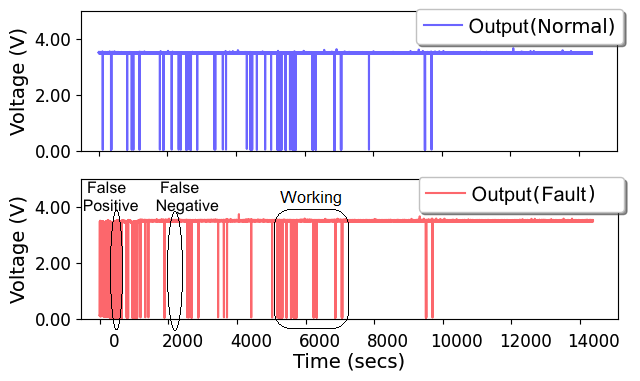
\includegraphics[width=0.5\textwidth]{figures/motivation/motivation-physics-technique.png}
	\caption{\footnotesize{Sensor Data} from a working PIR (top) and a faulty PIR (bottom). HIGH indicates no object, HIGH$\rightarrow$LOW transition indicates object.}
	\label{fig:occupancy_sensor_data}
\end{wrapfigure}




Currently, failures in PIR sensor deployments are usually addressed in one of the following two ways : \ca using an additional, auxiliary sensor such as a CCTV camera combined with image processing algorithms (say to validate the occupancy data) or \cb using high-grade PIR sensors that possesses additional capabilities such as ultrasonic sensors and intricate optics. This makes the sensor deployment very expensive. In addition, deployments need to be refreshed periodically by replacing old sensors with new ones and the former are disposed off adding to both electronic waste and cost. A case in point is our university research building where the occupancy sensor deployed is a high-grade PIR sensor comprising both ultrasonic and infrared sensors, resulting in a \emph{total recurring cost of close to \$100000 every 10 years}\footnote{Our 4-floor building (with a total of 244 rooms and 24 aisle areas) has more than 300 occupancy sensors. Each PIR sensor costs \$300~\cite{hubbell_ADT1600WRP, hubbell_ATD2000CRP} with it being refreshed every 10 years, a worst-case recurring cost of \$90000 every 10 years, which is expensive.}.




Crucially, \textit{current approaches do not diagnose the cause of failures or perform any analysis of sensor performance}, that can be valuable for IoT engineers during maintenance, repair and testing. For example, in one of our deployments, we observed that failed or degraded sensors can exhibit unpredictable behavior \eg they can work temporarily for a period of time and then fail sometimes. {\bfseries  Fig.~\ref{fig:occupancy_sensor_data}} shows a plot of output data from the sensor vs. time for both a working sensor and a faulty sensor (defective lens) over a period of 4 hours.
In this plot, a transition from HIGH$\rightarrow$LOW denotes a person coming into the field of view and a value of HIGH indicates that there is no person. We observe that the faulty sensor works intermittently and at other times, can miss a person (false negative) or incorrectly flag the presence of a person (false positive).
Missing a person can cause a potentially critical failure in applications such as door opening systems or emergency shutdowns on factory floors.
We show that accurate detection of such failures is possible by \textit{characterizing the internals of the sensor.}




\emph{Our solution, \sol detects and diagnoses failures of PIR sensors by characterizing the physics of sensing} \viz the fresnel lens optics and the pyroelectric effect. To keep the cost of the deployment low, \sol is implemented on the edge platforms of the deployment and targets commodity PIR sensors.
In this process, we \emph{devised a taxonomy of key failures for aiding diagnosis and repair.} 

Specifically, we demonstrate that a signal intrinsic to PIR sensors~\viz the \textit{intermediate analog output from the pyroelectric element, referred to as \aout} ({\bfseries Fig.~\ref{fig:pir_sensing_pipeline}}) can be used for fault detection and diagnosis. We utilize this signal to derive information about reliability of the PIR sensor platform as well as to perform an analysis into the different failure modalities. \textit{To the best of our knowledge, this is the first edge-based, low-cost approach to use an intrinsic signal (\aout) for fault detection and diagnosis of PIR sensors.} We analyze the behavior of \aout in detail, under practical deployments, with realistic occupancy
over a wide variety of observed failures. 

\noindent \textbf{Summary of Contributions:}
\begin{enumerate}[leftmargin=*]
	\itemsep0pt
	\item \textit{From physics to failures:} We use the working of a PIR sensor to understand the process of object detection and infer the key points where failures could lead to incorrect sensor data,
	\item \textit{Failure taxonomy:} We study the impact of different failures on the sensor performance and systematize the key failures into a failure taxonomy. We also provide a quantitative method to study the severity of failures.
	
	\item \textit{Non-intrusive, online fault detection and diagnosis:} We present an online technique (does not require any disassembling), \emph{implemented at the edge}, for failure detection as well as diagnosis by utilizing the intermediate, analog output from the pyroelectric element in the PIR sensor (\aout). 
	\item \textit{Insights from Real-world Deployments:} We show the efficacy of the proposed techniques using a deployment of 15 PIR sensors in four practical occupancy scenarios over a period of 3 months.
\end{enumerate}

\noindent \textbf{Goals:}
\begin{enumerate}[leftmargin=*]
	\itemsep0pt
	
	\item {\itshape Detect failures:} Sensors can give faulty data due to the incorrect operation of various physical components involved in the sensing process. We seek to detect and isolate such failed sensors. 

	\item {\itshape Diagnose failures:} In addition to detecting failures, we perform failure diagnosis to identify the cause of the failure. We use domain-knowledge of the sensing physics and our understanding of how different failures can impact the physics. This aids in repair and performing quality-control checks.
	
	\item {\itshape Edge-based solution:} \sol is tailored for edge platforms (Raspberry Pi, Arduino Microcontrollers) that are interfaced directly to multiple sensors, say via GPIO. Edge-based reliability solutions allows us to reject data from faulty sensors in IoT deployments thus saving the cost of both \ca the edge to cloud network bandwidth and \cb cloud compute consumed by faulty data.
	
	\item {\itshape Target Audience:} \sol benefits two sections of the community: \ca engineers developing and deploying IoT/Edge computing for occupancy sensors (\eg Smart Buildings), \cb manufacturers of occupancy sensors can use the insights from this work towards future PIR sensor hardware designs.
	
\end{enumerate}


 \section{Related Work} 
\label{sec:related}







Current solutions for failure detection and diagnosis in sensors fall into one of three categories -- \ca Data-driven techniques, \cb Calibration-based techniques and \cc Fingerprint-based techniques.

\textbf{Data-driven techniques.} Prevalent research efforts have largely focused on data-centric approaches (rule-based or anomaly detection), where historical data of the sensor is analyzed and a fault is identified if the data is out of bounds of the expected behavior~\cite{rashid2016collect, 10.1145/3365871.3365872}.  Sharma~\etal~\cite{10.1145/1754414.1754419}, proposed a multiplicative seasonal ARIMA time series model for fault detection, where the parameter captures periodic behavior in the sensor data. The downside of temporal analysis methods is that
they are prone to false positives and are not feasible in long-term
deployments. Wu~\etal~\cite{4262542} used a spatial mining-based approach that uses spatial correlation between neighboring sensors to detect anomalies. Additionally, techniques such as Ayadi~\etal~\cite{7505190}, Murphree~\cite{7589589} and Power~\etal~\cite{10.1145/3365871.3365872} require significant labeled data as it models only the environment and does not model the sensor physics. Estimation-based methods model normal sensor behavior leveraging spatiotemporal correlation and probabilistic models such as Bayesian or Gaussian distributions~\cite{10.1145/1140104.1140114} and they work well in homogeneous environments. In a nutshell, the key challenge with data-driven techniques is that it relies on rules and patterns in the sensed data.
We argue that for PIR sensors since the data is non-periodic and dependent on deployment scenarios (\eg people counting in Starbucks,   
animal detection in forests, etc.), \textit{it is non-trivial to detect faults by just analyzing sensor data.} Further, this requires significant manual efforts and tailor-made rules to detect faults, and can eventually have high false positives due to unseen data patterns. Additionally, data-driven techniques do not provide information about the specific nature or degree of failure in the sensor. As a result, they do not aid in the process of developing repair strategies. This is also seen in works such as Tawakuli~\etal~\cite{tawakuli2023experience}, that discusses the repercussions of missing data to be of two types -- \ca isolated missing data and \cb sequence missing data. They develop a domain-independent, dataset-independent, hybrid imputation strategy that can give better estimation accuracy by looking at six real-world datasets such as AirQuality and NASDAQ time-series data. Tawakuli~\etal~\cite{Tawakuli2022TransformingID} describes a generic edge-cloud IoT-based preprocessing framework targeting AI pipelines. The framework comprises steps such as data cleaning and feature engineering, and can leverage \sol to assist in cleaning data associated with faulty PIR sensors. In summary, data-driven techniques, while scalable, often entail substantial labeling efforts, leading to high costs, and can exhibit low accuracy due to their dependence on custom rules and patterns. Moreover, they provide no guidance on correcting faulty sensors, as they disregard the underlying physics of sensing.

\textbf{Calibration-based techniques.} These techniques rely on the presence of an additional (reference) sensor, either to perform periodic calibration~\cite{whitehouse2002calibration, 8405565} or carrying additional information in a different domain space.  \Eg using a camera to cross-check the data of a PIR sensor~\cite{tang2017occupancy}. Numerous algorithms have been developed for performing calibration such as blind calibration~\cite{7472216, 7495010}, collaborative calibration~\cite{10.1145/2737095.2737113, 10.1145/2185677.2185687} and transfer calibration~\cite{article_nose}. Agarwal~\etal~\cite{Agarwal2021ANA} uses temperature and power consumption data to infer if a HVAC is faulty or working. It relies on the correlation between the two individual data streams from auxiliary sensors~\viz smart meters and temperature sensor. By studying such a relationship between multiple sensors, Agarwal~\etal~\cite{Agarwal2022ANA} provide a optimization framework to minimize the number of sensors required to sense a facet such as occupancy. Their framework uses fault tolerance information in their framework and, in such a setting, \sol can be used to minimize the number of sensors in a Building Management System (BMS), thereby lowering operational costs and improving efficiency. Huchuk~\etal~\cite{huchuk2021data} develop a machine learning model based on data from thermostats to predict set points overrides that happen across a set of buildings, helping create more energy efficiency schemes. They note that using building-level indoor conditions will help create more energy efficient schedules and \sol can aid in improving the accuracy of such systems. However, all of these approaches that use reference sensors are expensive and lacks scalability for large IoT deployments. 

\textbf{Fingerprint-based techniques.} Chakraborty~\etal~\cite{chakraborty2018fall} develop a sensor signature~\viz ``Fall Curve'' that measures a sensor's voltage response when the power is turned off, to detect faults in periodic on-off based analog sensors. 
The Fall Curve characterizes the parasitic capacitance and hardware circuitry of the sensor. Crucially, Chakraborty \etal show this signature is unique for every sensor type and is independent of the environment. They demonstrate that this approach works well for sensors that have very little or no warm-up time and work in a periodic on-off fashion. 
Furthermore, Chakraborty \etal \cite{chakraborty2018fall} point out to the fact that extending this approach to digital sensors where one doesn't have direct access to the analog signal is challenging. Additionally, Fall Curve is complex in sensors having low value of operating voltages and lack periodicity in the sensing mechanism. Our work concerns this design space of exploring faults in discrete-valued PIR sensors. PIR sensors are challenging since in addition to being discrete valued, the internal analog signal~\viz output from the pyroelectric element has a very low value. 
Similarly, Tambe~\etal~\cite{10.1145/3458864.3466869} show a variant of Fall Curve~\ie ``Fall Time'' of the analog signal can detect faults and drifts in phototransistor components of the sensor.
However, both Fall Curve and Fall Time signatures do not work on certain types of sensors including PIR, that operate under low voltages and are event-triggered. Marathe~\etal~\cite{marathe2021currentsense} show that analyzing the current profiles of a digital sensor can provide insights into component failures especially in electro-mechanical sensors. However, this approach is limited to power-hungry digital sensors. Gupta~\etal~\cite{10.1145/3576842.3582386} develop a Verified Telemetry SDK (VT-SDK) constructed on robust sensor fingerprinting algorithms and demonstrate fault detection on multiple sensors ranging from air pollution to pressure sensors.
There are other hardware-based techniques such as Liu~\etal~\cite{Liu_Huang_Luo_Harkin_McDaid_2019} that detects electronic faults by developing additional circuits inspired by the biology of neurons.
In summary, fingerprint-based techniques have been applied to sensors such as air pollution, smoke, and soil temperature and moisture sensors but have not been extended to PIR sensors.

PIR sensors are challenging since in addition to being discrete-valued, the internal analog signal output from the pyroelectric sensor has a very low value, often oscillating between 1--1.8V. We show that the intermediate analog output (\aout) from the PIR sensor carries interesting insights on the characteristics of the sensor. Narayana~\etal~\cite{narayana2015pir} leveraged this signal by developing a customized sensor array for performing localization and studying object metrics. They develop a customized sensor tower consisting of a strategic geometric arrangement of multiple PIR sensors to enable capturing the analog signal from those multiple sensors. They use this to study the object size (height and width) and posture (such as its distance from the sensor and the direction of motion) and its impact on features of the analog signal such as frequency, amplitude, phase and time difference between peaks. 
However, Narayana~\etal~\cite{narayana2015pir} do not explore reliability.












 
\section{PIR Sensors}
\label{sec:approach}
We take a deep dive into a PIR sensor with 3 goals -- \ca understanding the physics of sensing (\S\ref{subsec:physics}, \S\ref{subsec:working}), \cb correlating physics to the failure scenarios (\S\ref{subsec:taxonomy}) and \cc analyzing the effect of these failures on the sensing performance (\S\ref{subsec:quantify}).


\subsection{Background}
\label{subsec:physics}
The teardown of a PIR sensor, showing the internal components is shown in {\bfseries Fig.~\ref{fig:pir_system_teardown}}.
It comprises 3 subsystems -- \ca a lens, \cb a pyroelectric attached to an optical filter, and \cc an electronic subsystem.
These subsystems act in sequence \ie Lens $\rightarrow$ Pyroelectric $\rightarrow$ Electronic to perform the end-to-end sensing process as shown in {\bfseries Fig.~\ref{fig:pir_sensing_pipeline}}. We describe the different subsystems next.

\noindent \underline{\bfseries Lens Subsystem} A plastic fresnel lens~\cite{an_murata} is used to capture and precisely focus thermal radiation into an optical filter that is aimed at a pyroelectric element. 
Fresnel lenses have a large capture area (aperture) and are used to concentrate radiation into a narrow beam. They are used to divide the entire region observable to the PIR sensor into small cells, which increases range of the sensor by manifolds. 
They have a large capture area (aperture) and are common in a wide variety of applications such as lighthouses, solar cells and even in optical landing systems in aircrafts~\cite{webster1999measurement}.
\begin{wrapfigure}{lr}{0.25\textwidth}
	\centering
	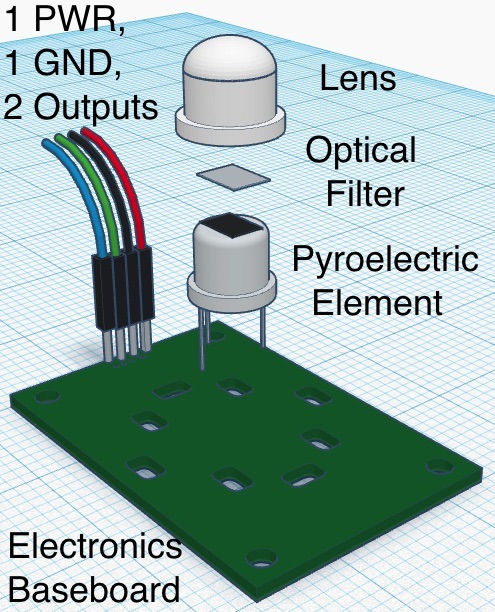
\includegraphics[width=0.2\textwidth, height=1.3in]{figures/platform/3d_view_5-annotated.jpg}
	\caption{PIR Sensor Teardown showing the different subsystems illustrated in TinkerCAD}
	\label{fig:pir_system_teardown}
\end{wrapfigure}
\noindent \underline{\bfseries Pyroelectric Subsystem} comprises of an optical filter and a pair of pyroelectric elements. The optical filter is designed to filter out thermal radiations from wavelengths outside the human range (i.e., ~ 5 $\mu$m to 10 $\mu$m), which is then incident on the pyroelectric elements. The pyroelectric elements convert the thermal radiation into an electrical voltage signal, a process known as the \textit{pyroelectric effect}. The output of the pyroelectric subsystem is an analog signal that is sent to the electronic subsystem.
In practice, there are two pyroelectric elements connected in series in a differential configuration. This differential configuration enables the PIR sensor to detect \textit{movement} of objects as static objects will trigger both the pyroelectric elements equally and cancel out unlike moving objects that trigger both elements unequally resulting in an output from the pyroelectric subsystem. Due to the differential output voltage, the pyroelectric subsystem does not measure the absolute intensity of incident thermal radiation but measures a change in incident thermal radiation, say caused by motion. Note that the pyroelectric element by itself is passive \ie has no power source.


\noindent \underline{\bfseries Electronic Subsystem} consists of a filter (RC filter), amplifier (JFET or OpAmp) and comparator (OpAmp) circuits. The output from pyroelectric subsystem are filtered to remove noise, amplified to increase its magnitude and finally sent to a comparator to convert analog signals to discrete signals. This \textit{discrete signal is HIGH when there is no motion and goes HIGH$\rightarrow$LOW when motion is detected}. Systems connected to a PIR sensor such as lighting or heating use the discrete signal to regulate the illumination or temperature in a building.


\subsection{\textbf{Analysis of Output Signals of a PIR Sensor:}}
\label{subsec:working}
There are 2 output signals from a PIR sensor as shown in {\bfseries Fig.~\ref{fig:pir_sensing_pipeline}}:
\begin{enumerate} \item \textbf{Final discrete output} of the electronic subsystem (\cout) that follows negative logic \ie stays HIGH when there is no motion and goes LOW when motion is detected. \item \textbf{Intermediate analog output} just prior to the discretization process (\aout). \end{enumerate}\begin{figure}
	\centering
	\begin{subfigure}[b]{0.4\textwidth} \begin{flushleft}
			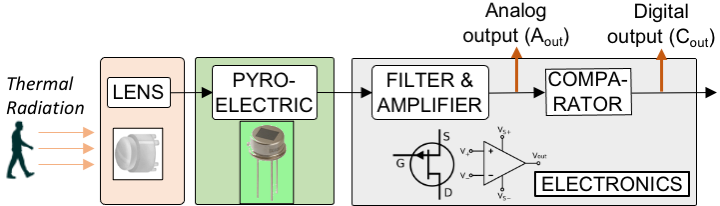
\includegraphics[width=\textwidth]{figures/platform/pir-block-diagram-2-redraw-camera.png}
			\caption{Sensing Pipeline of a PIR Sensor}
			\label{fig:pir_sensing_pipeline}
		\end{flushleft}
	\end{subfigure}\hfill
	\begin{subfigure}[t]{0.3\textwidth}
		\centering
		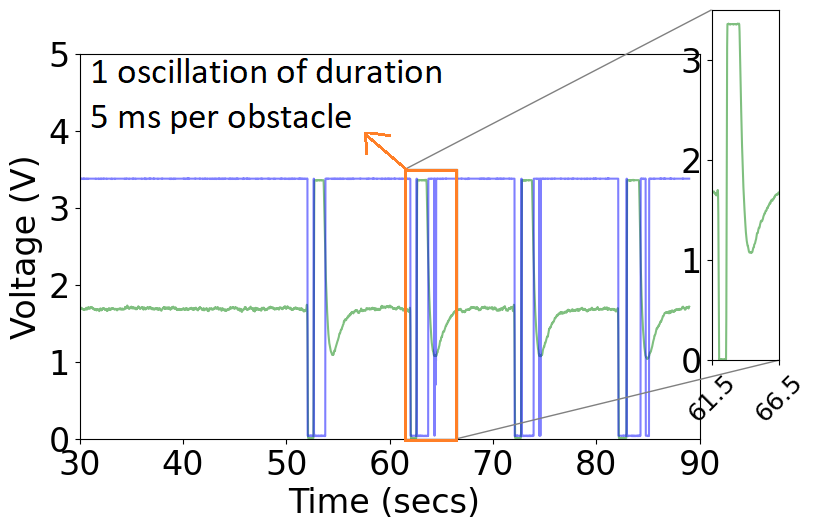
\includegraphics[width=\textwidth]{figures/lens_types/inline_lens.png}
		\caption{Inline lens (wall-mount)}
		\label{fig:inline_lens}
	\end{subfigure}\begin{subfigure}[t]{0.3\textwidth}
		\centering
		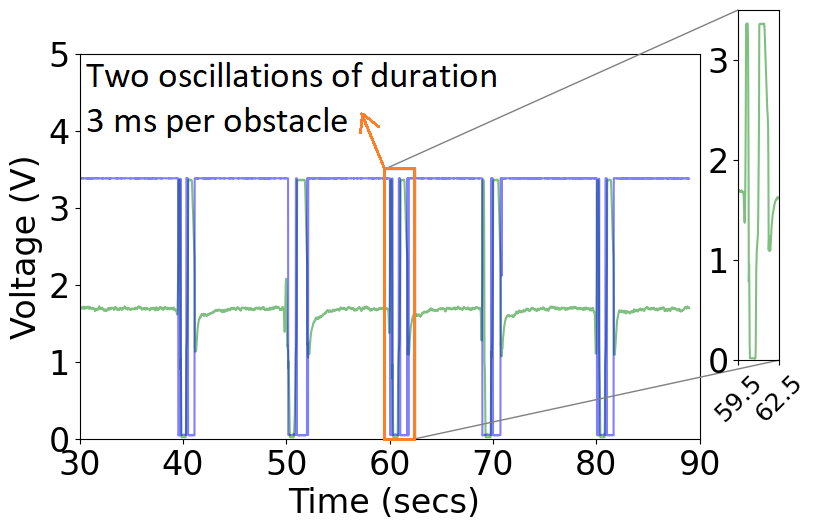
\includegraphics[width=\textwidth]{figures/lens_types/round_lens.png}
		\caption{Round lens (ceiling-mount)}
		\label{fig:round_lens}
	\end{subfigure}	   
	\caption{Effect of different types of lens on the \aout curve, shown in green -- the inline lens type produces a single oscillation whereas a round lens type produces two oscillation per obstacle. The corresponding \cout, shown in blue, stays HIGH when there is no motion and goes LOW when motion is detected. }
	\label{fig:pir_sensor_different_lens}
\end{figure}To analyze \cout and \aout during operation, we interface a PIR sensor to an Arduino microcontroller~\cite{arduino_mega}. 
{\bfseries Fig.~\ref{fig:inline_lens} --~\ref{fig:round_lens}} shows plots of \aout and \cout for a period of 60 seconds, both in the presence and absence of an obstacle. The y-axis represents voltages seen at the output and x-axis represents time. As expected, \cout, marked in blue, goes LOW when an obstacle comes into the field of view and stays HIGH otherwise. On the other hand, \aout, marked in green, measures around 1.8 V when there is no obstacle and produces oscillation(s) when an obstacle comes into the field of view (shown magnified). 
The nature and shape of the \aout curve also depends on the nature of lens used in the PIR sensor. Typically, an inline lens is used for the wall-mount version and a round lens is used for the ceiling-mount version. {\bfseries Fig.~\ref{fig:pir_sensor_different_lens}} also shows the variations in \aout between the two lens types -- \ca Inline lens has a wider curve compared to round lens and \cb Round lens has double number of oscillations of \aout curve per obstacle. We used a wall-mount PIR sensor in our experiments though our analysis, techniques and observations are equally applicable to ceiling-mount sensors. With a working background on PIR sensors, we next study the various failures in a PIR sensor and its impact on sensing physics. \subsection{Failures in PIR Sensors -- A Taxonomy} 
\label{subsec:taxonomy} 

Fundamentally, failures in a PIR sensor could occur either on the lens, the pyroelectric element or the electronics. We \textit{analyze and categorize practical, common and most frequent} failures as gathered in discussions with IoT engineers and technicians who install and maintain PIR sensor deployments. 
We developed a new taxonomy for such failures, as summarized in {\bfseries Table~\ref{tab:pir_faults}} and visualized in {\bfseries Fig.~\ref{fig:pir_sensor_failure_photographs}}.\subsubsection{\textbf{Failures in the lens subsystem}} The lens is geometrically constructed to precisely focus the thermal rays onto the pyroelectric element. As a result, failures affecting the optical integrity of the lens can result in loss of precision for focusing the thermal rays. We observe three types of failures here, termed Class I--III failures.


\noindent \underline{Lens dislocation (Class I):} As the lens is stuck on the sensor board with an adhesive or machined to fit over the pyroelectric element, it could get dislodged from its place or completely fall off the sensor board due to factors such as thermal expansion or physical impact.

\begin{figure}\centering
	\small
	\begin{subfigure}[t]{0.24\textwidth}
		\centering
		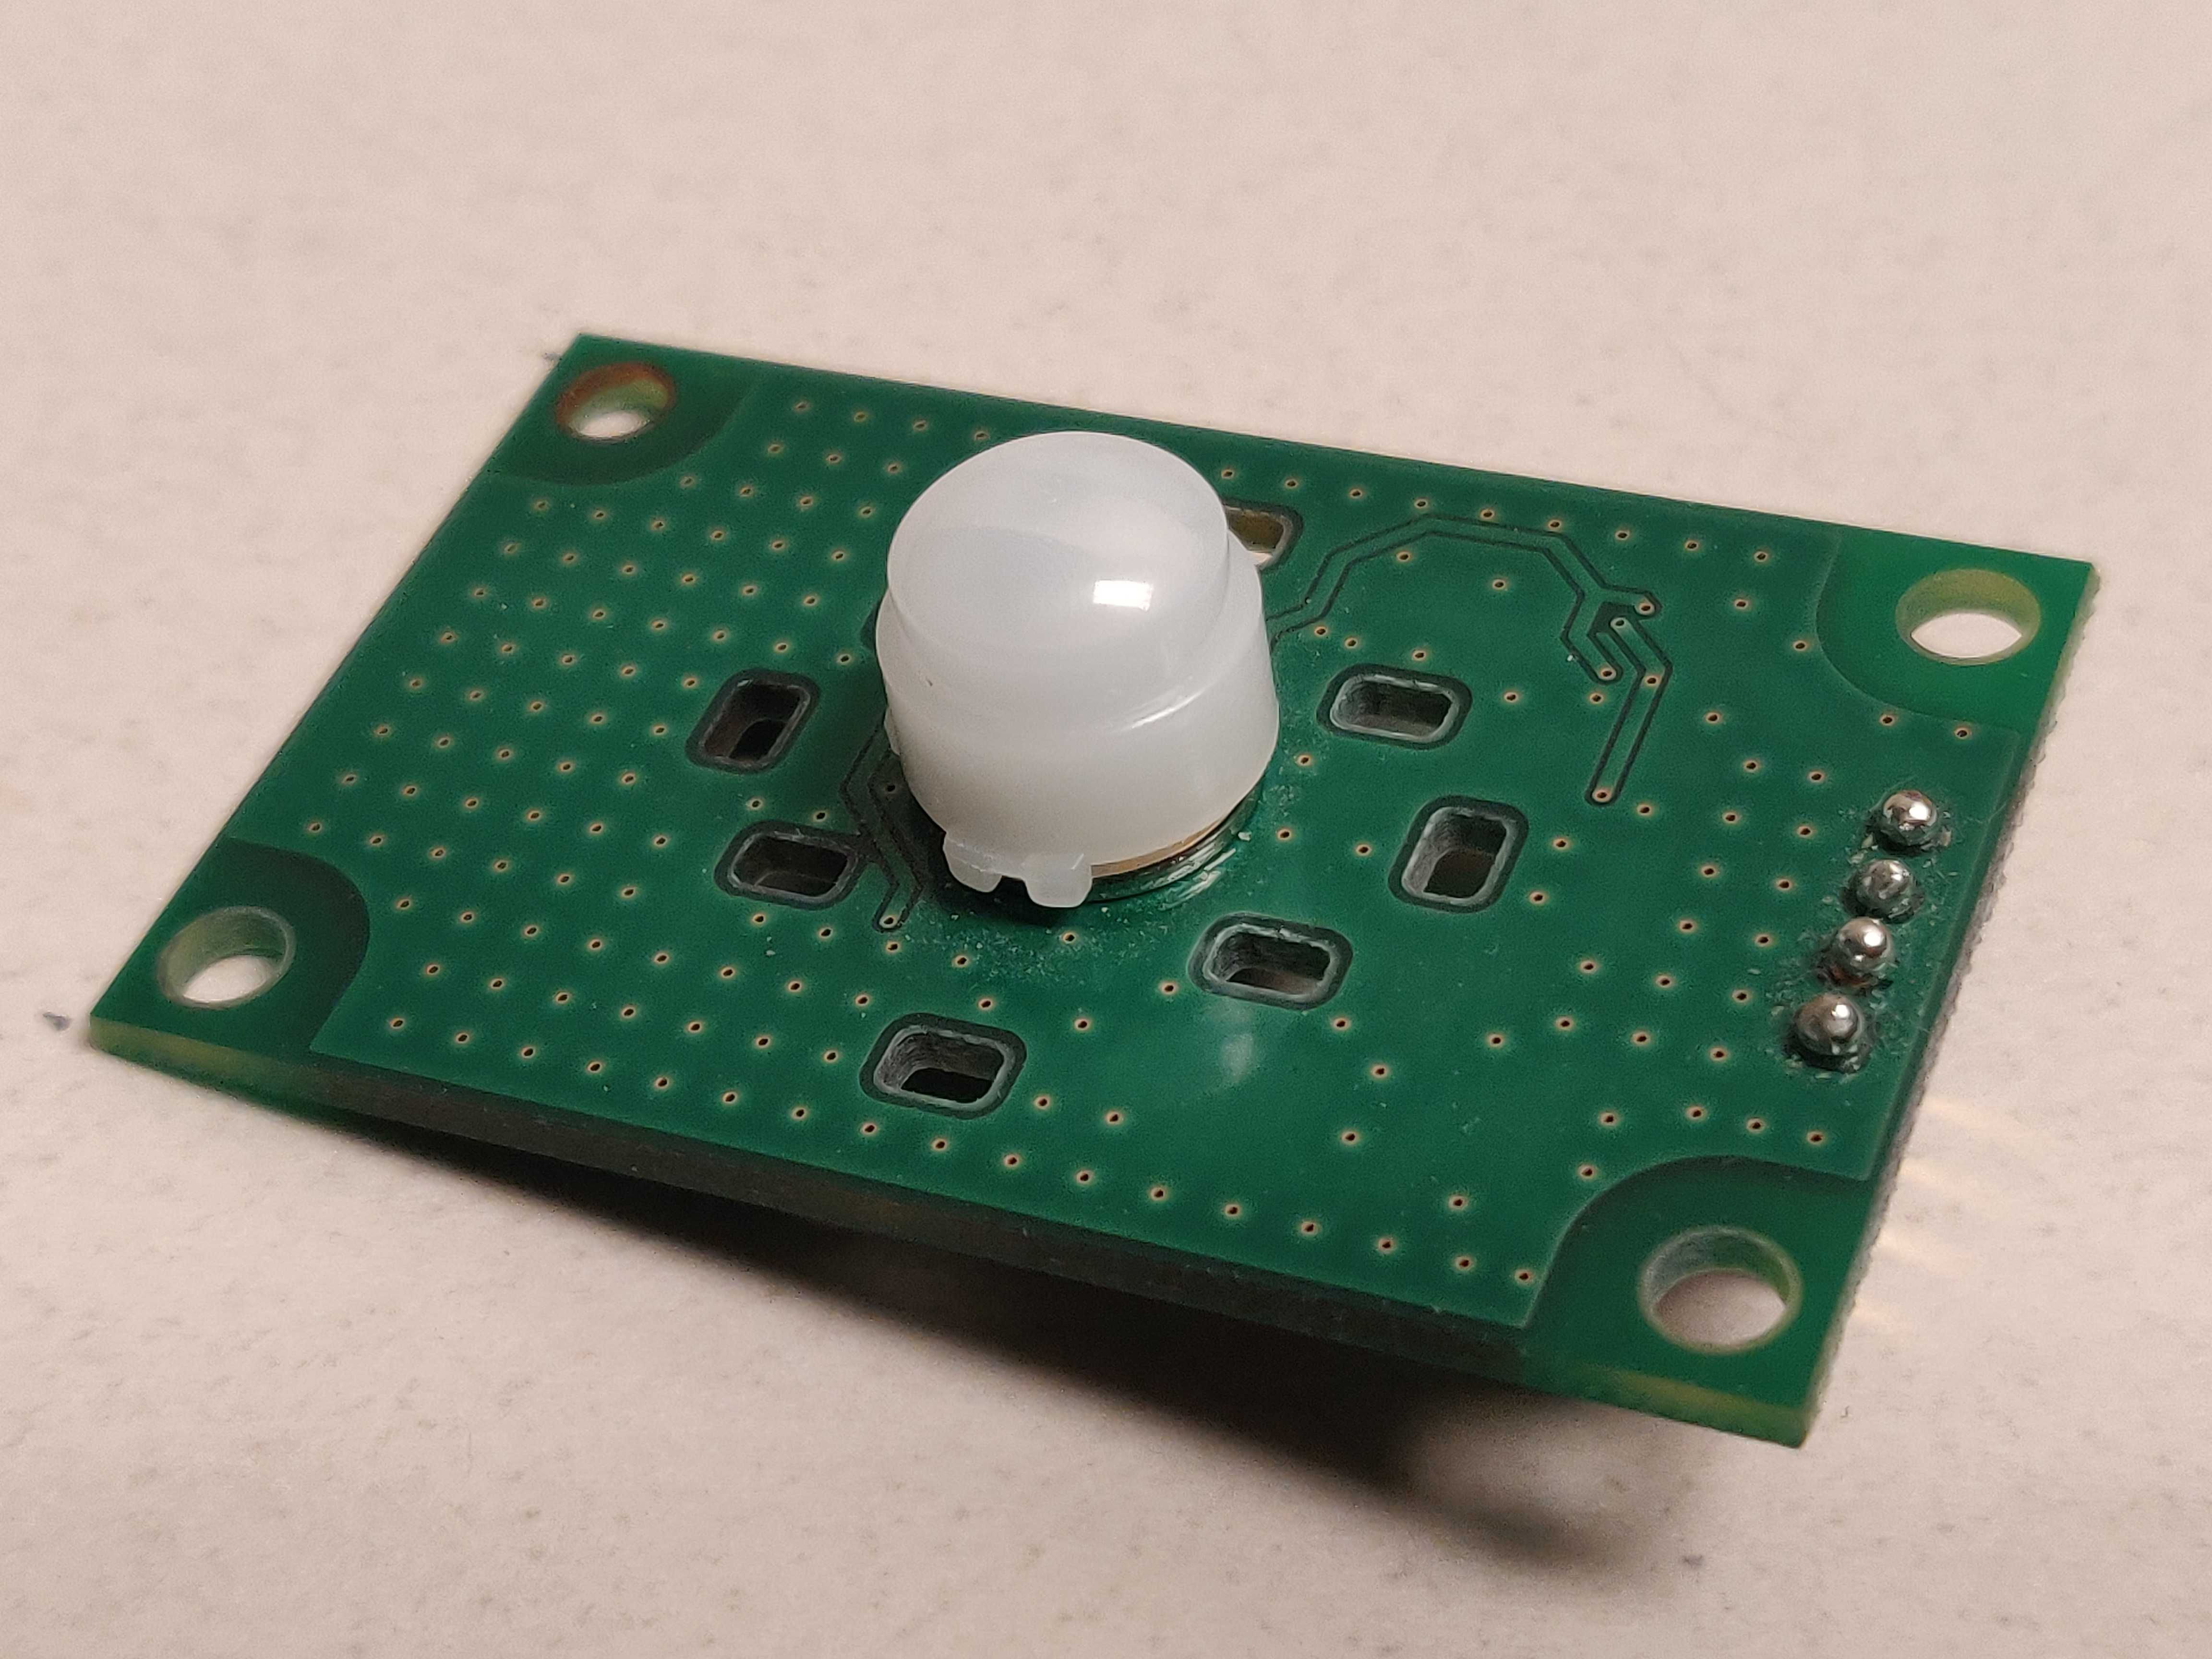
\includegraphics[width=\textwidth]{figures/platform/failure_photographs/WorkingSensor-proper.jpg}
		\caption{\footnotesize Working Sensor}
		\label{fig:working}
	\end{subfigure}
	\hspace{0.10ex}\begin{subfigure}[t]{0.24\textwidth}
		\centering
		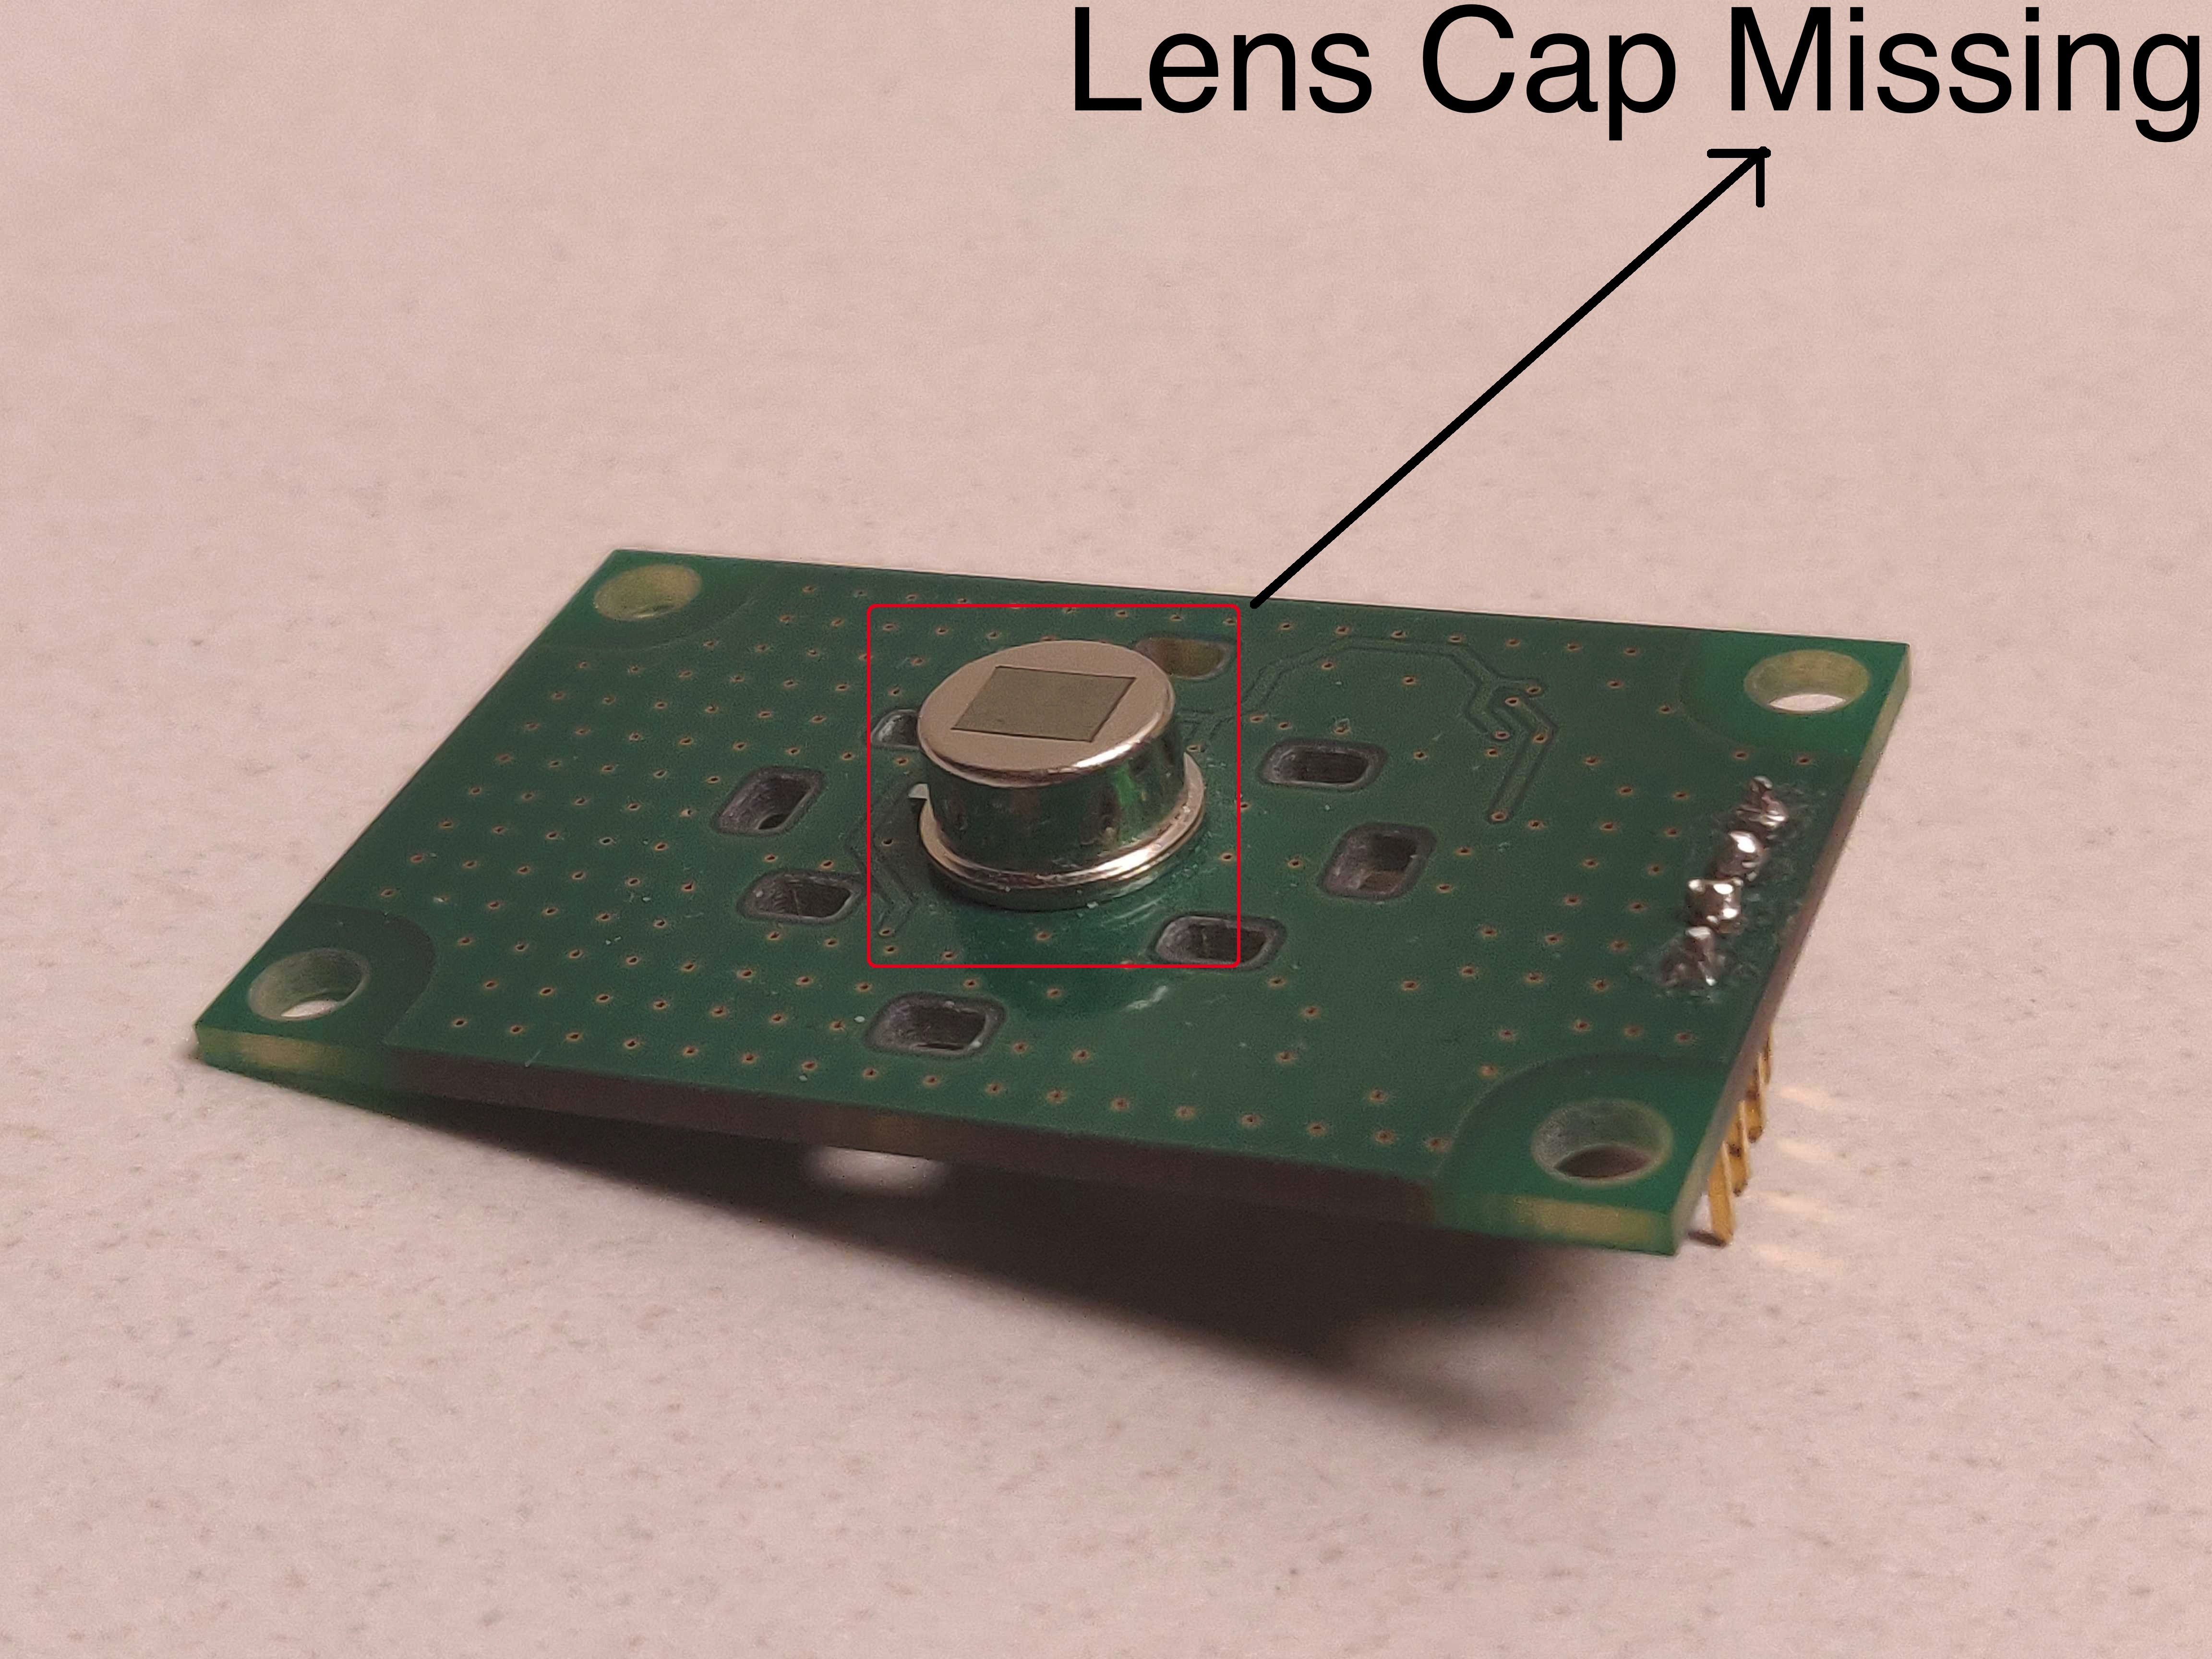
\includegraphics[width=\textwidth]{figures/platform/failure_photographs/ClassI-LensCapRemoved-annotated-jpg.jpg}
		\caption{Lens Cap Fallen Off}
		\label{fig:failure_photo1}
	\end{subfigure}
	\hspace{0.10ex}
	\begin{subfigure}[t]{0.24\textwidth}
		\centering
		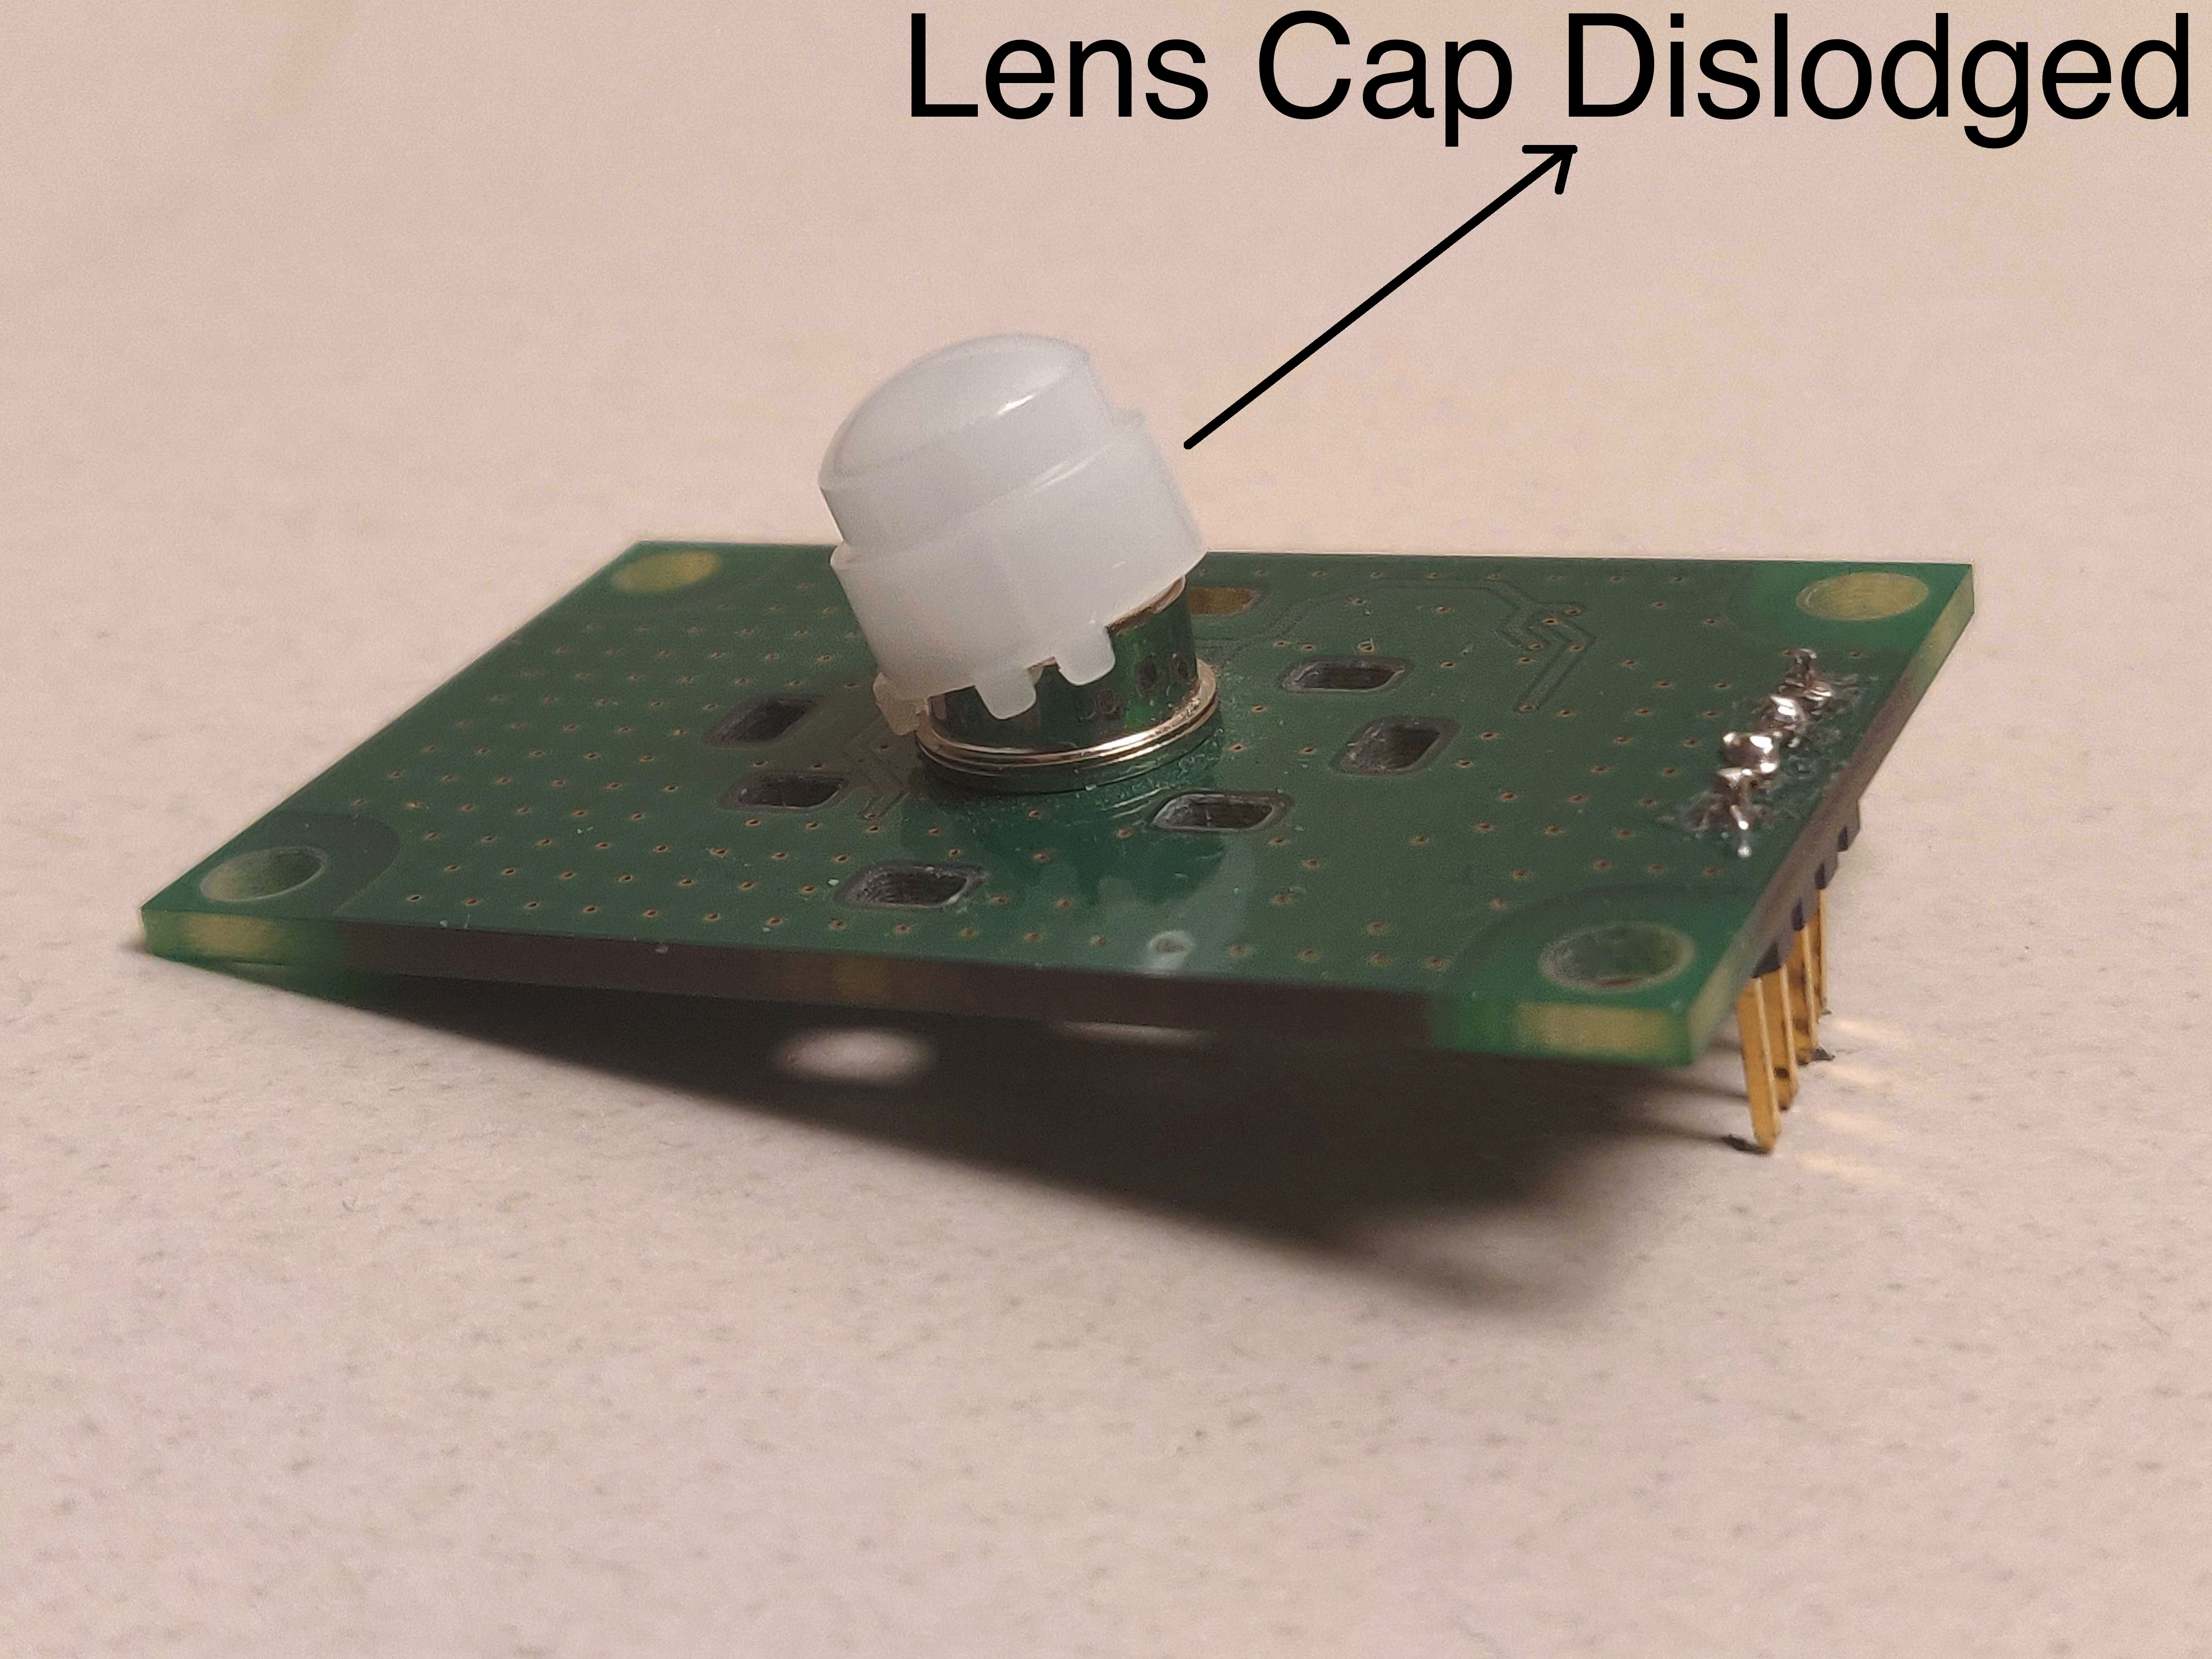
\includegraphics[width=\textwidth]{figures/platform/failure_photographs/ClassI-LensCapDislogdged-annotated-jpg.jpg}
		\caption{\footnotesize Lens Cap Dislocated}
		\label{fig:failure_photo2}
	\end{subfigure}	
	\hspace{0.10ex}
	\begin{subfigure}[t]{0.24\textwidth}
		\centering
		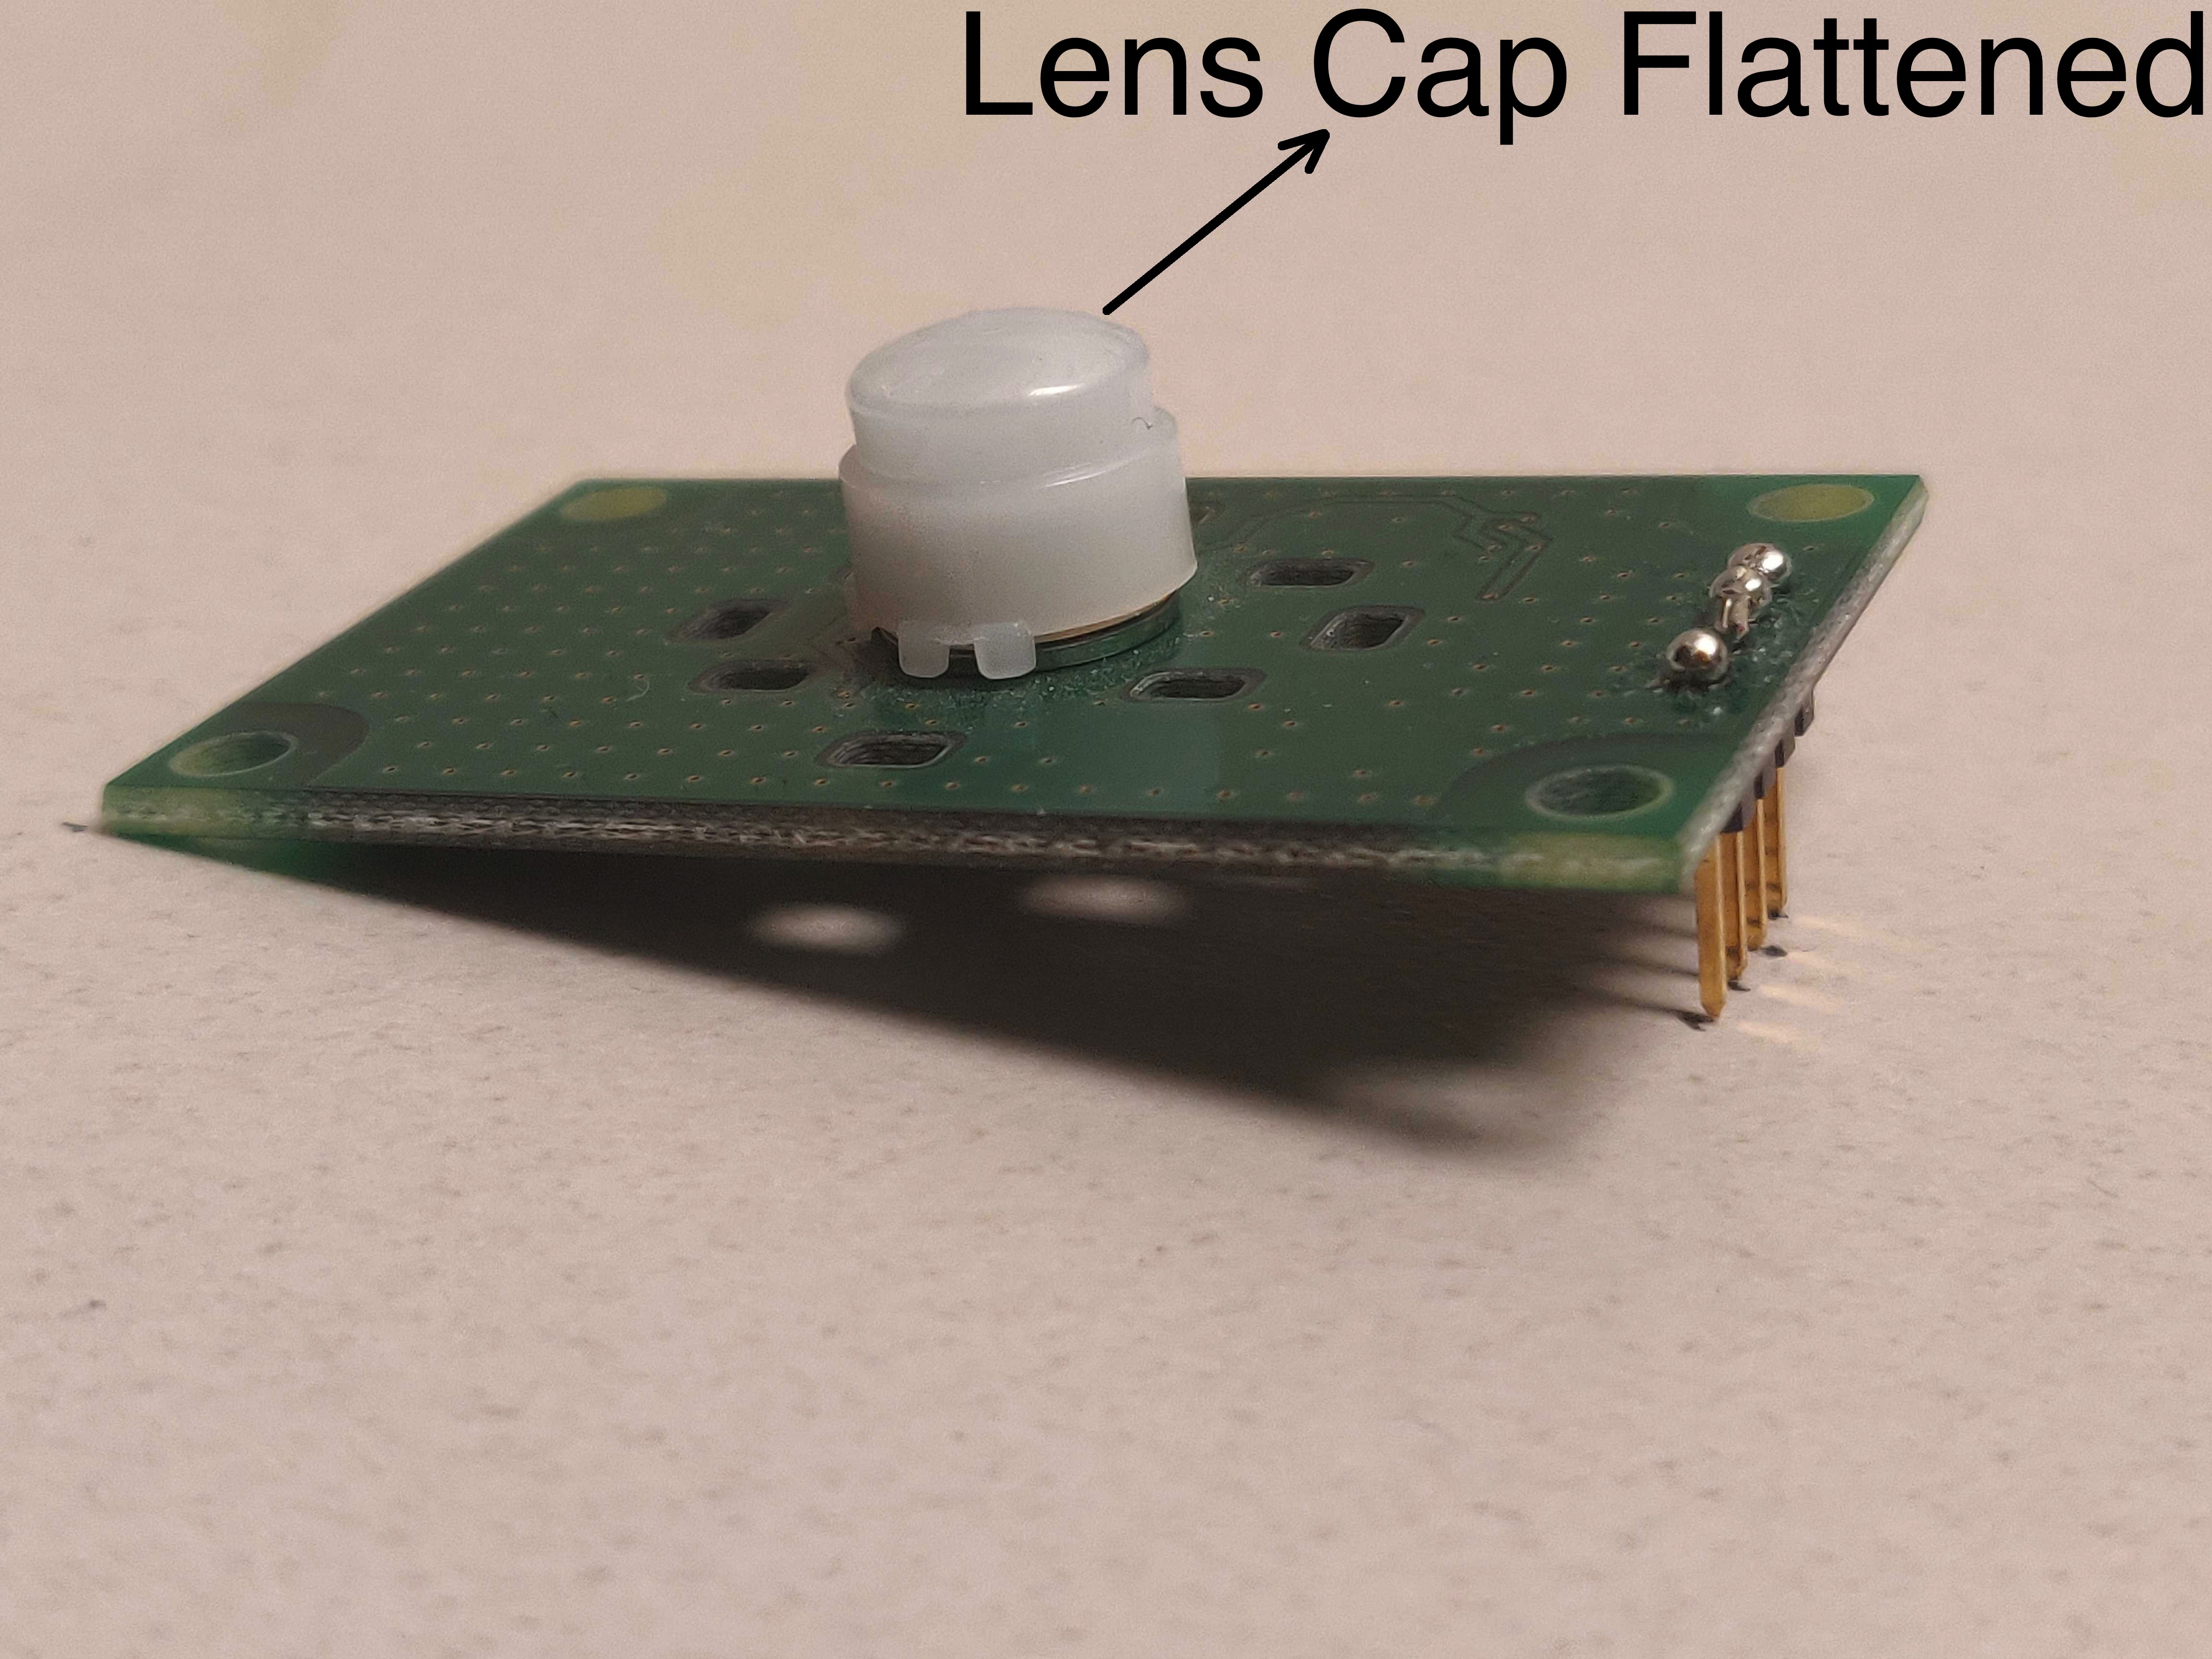
\includegraphics[width=\textwidth]{figures/platform/failure_photographs/ClassII-LensCapDeformed-annotated-jpg.jpg}
		\caption{Lens Cap Deformed}
		\label{fig:failure_photo3}
	\end{subfigure}
	\begin{subfigure}[t]{0.24\textwidth}
		\centering
		\includegraphics[width=\textwidth]{figures/platform/failure_photographs/ClassII-LensCapPunctured_new-2-annotated.png}
		\caption{Lens Cap Punctured}
		\label{fig:failure_photo4}
	\end{subfigure}
	\hspace{0.1ex}
	\begin{subfigure}[t]{0.24\textwidth}
		\centering
		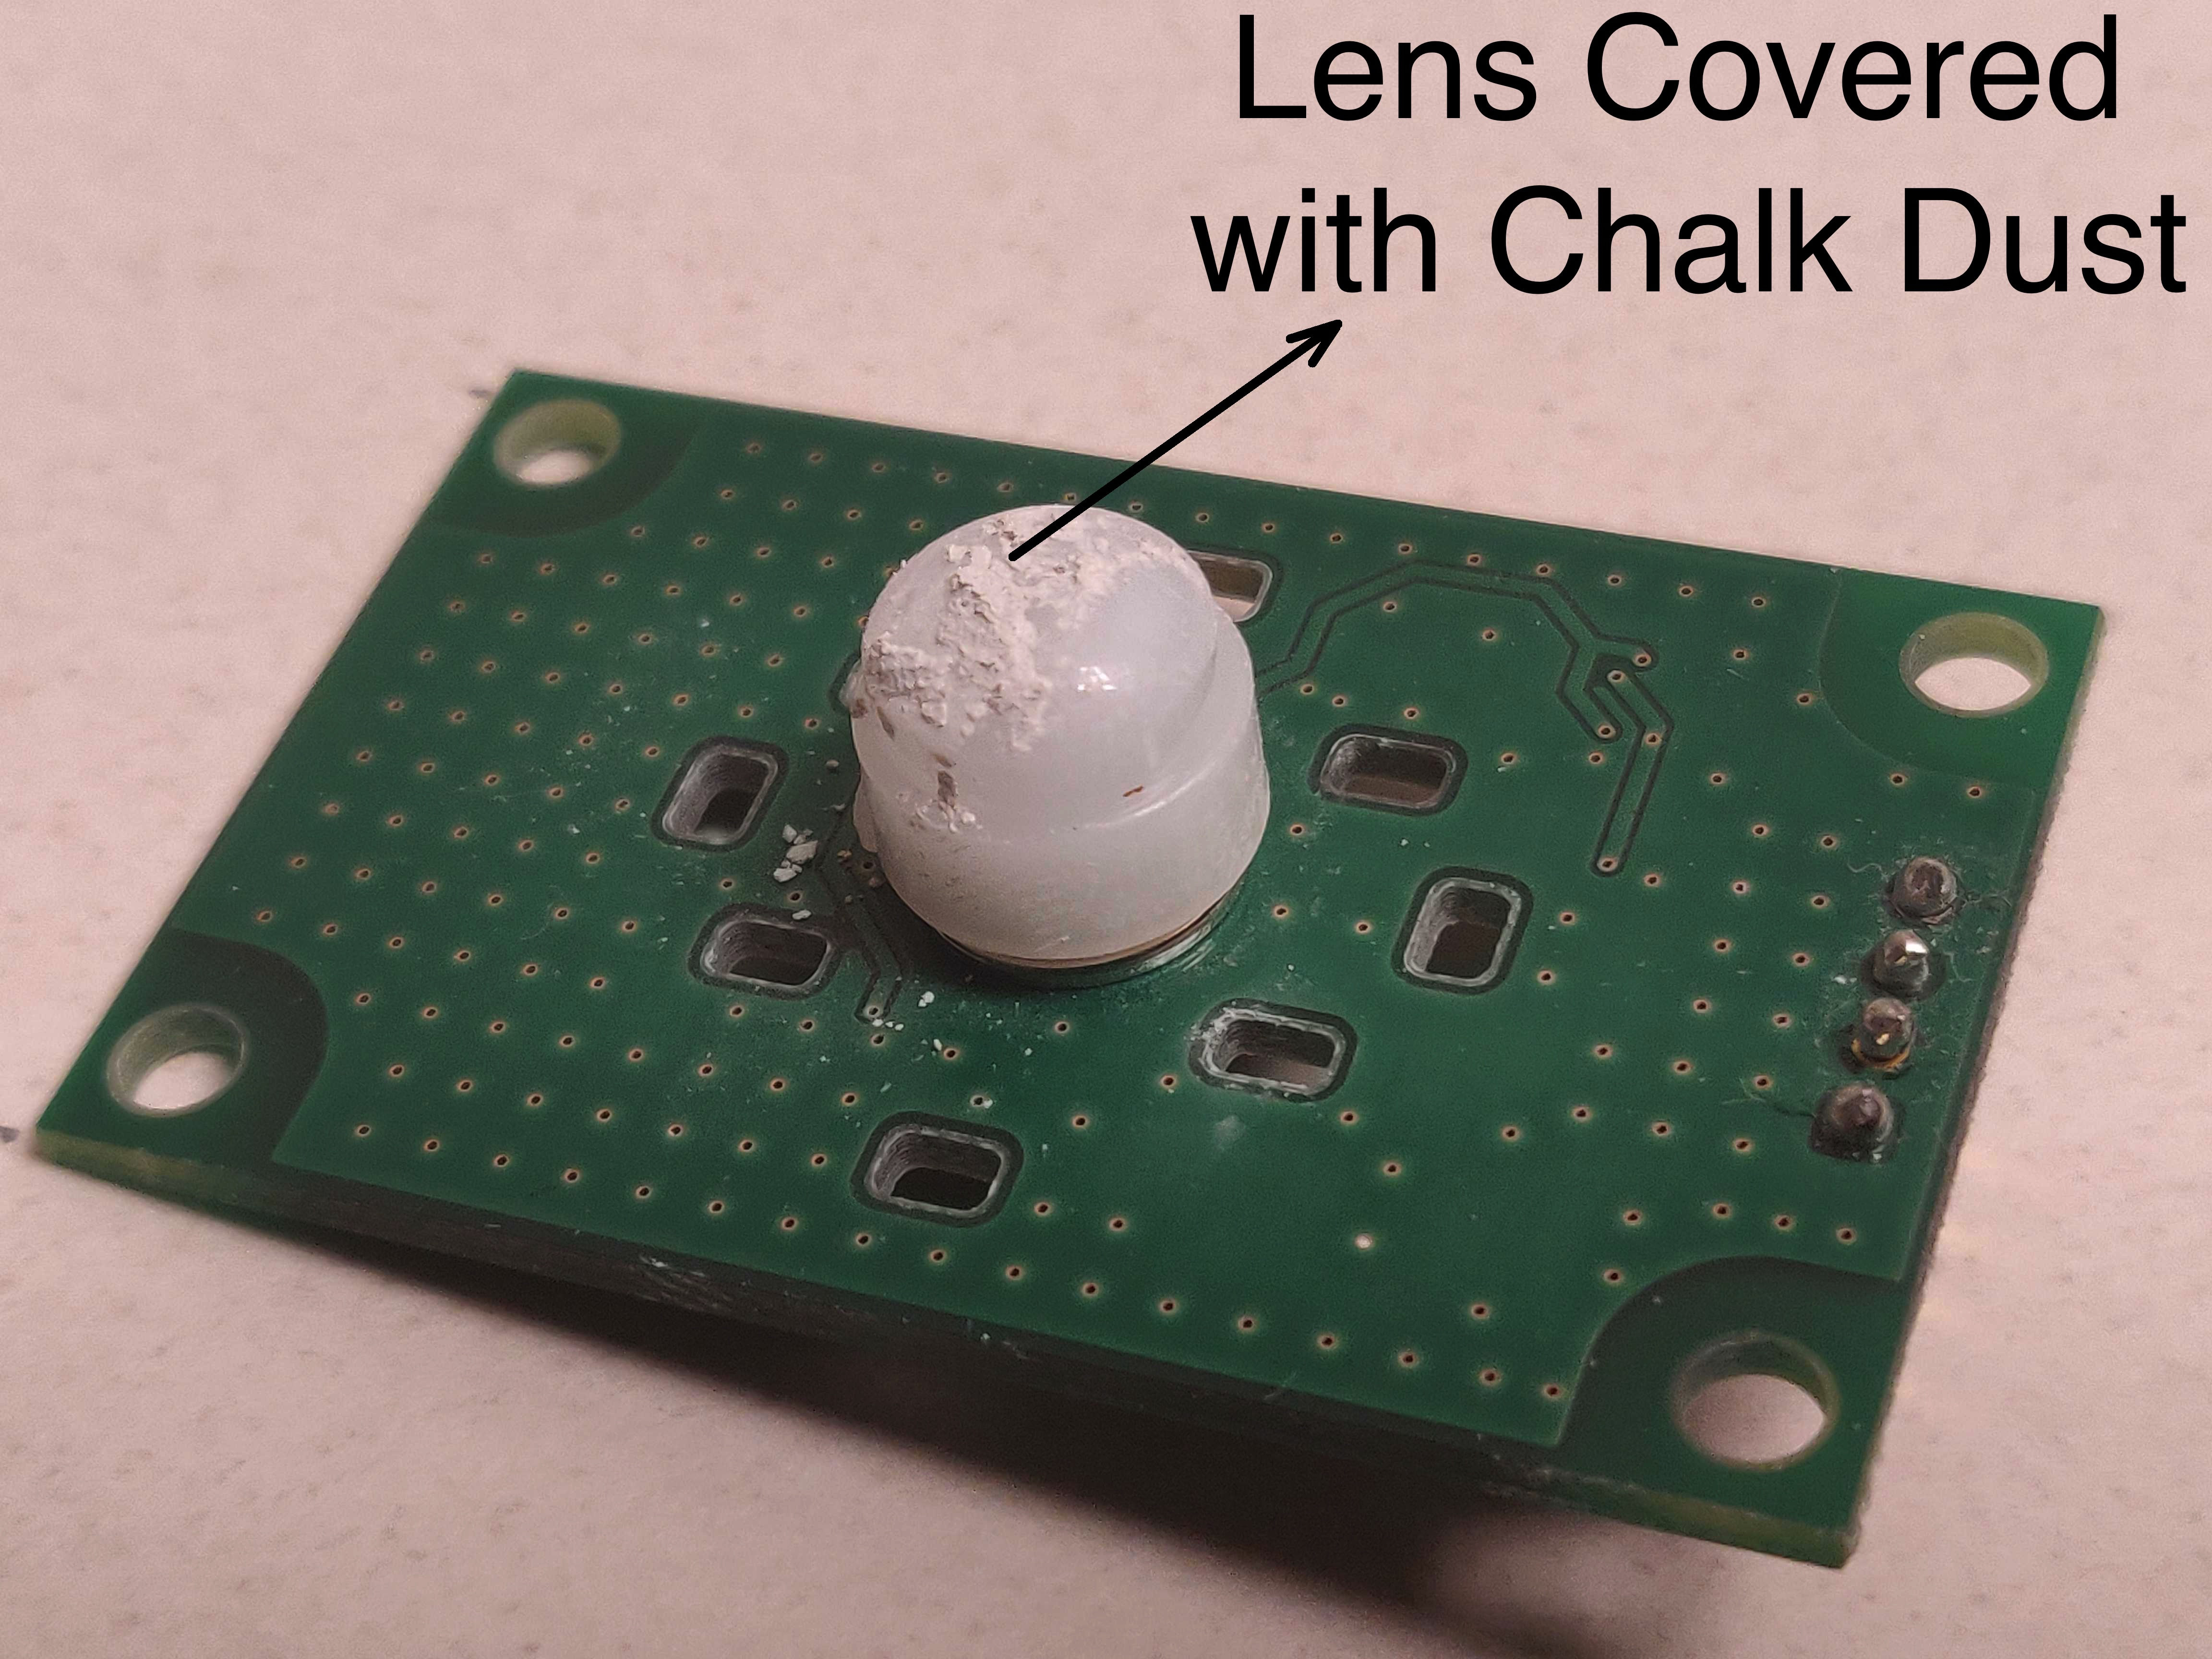
\includegraphics[width=\textwidth]{figures/platform/failure_photographs/ClassIII-LensCapCovered-annotated-jpg.jpg}
		\caption{\footnotesize Lens Cap Covered}
		\label{fig:failure_photo5}
	\end{subfigure}
	\hspace{0.1ex}\begin{subfigure}[t]{0.24\textwidth}
		\centering
		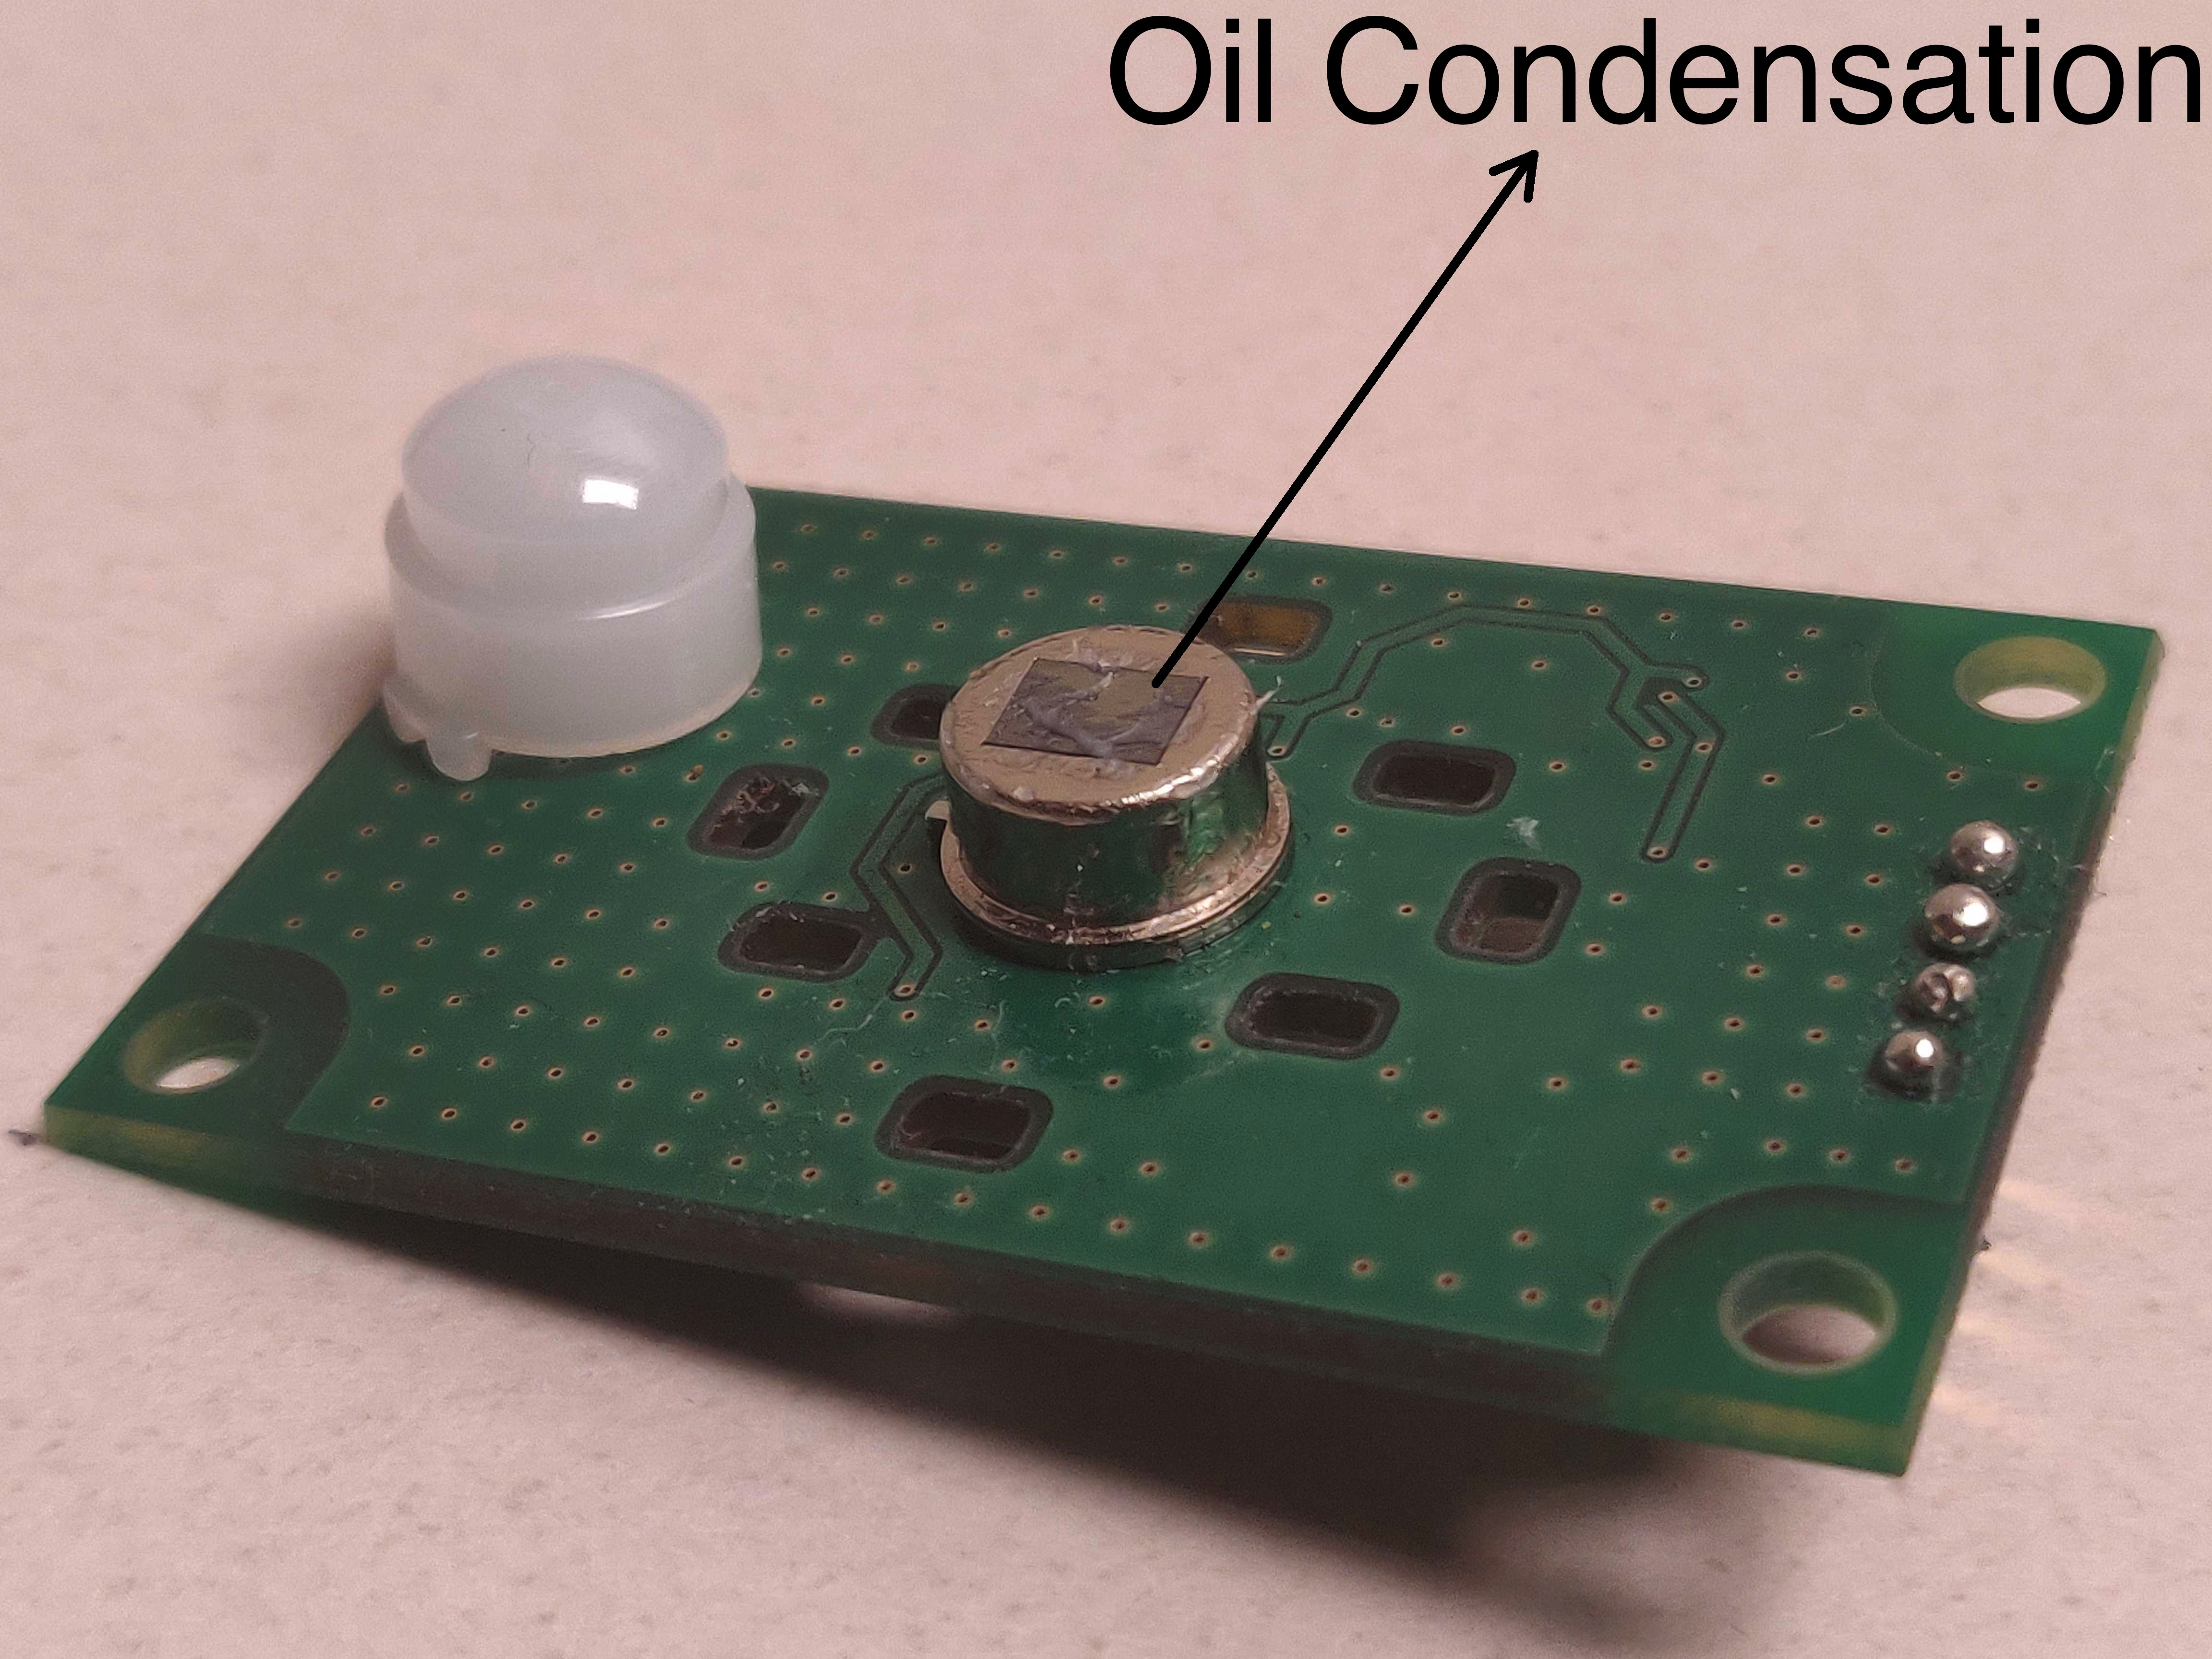
\includegraphics[width=\textwidth]{figures/platform/failure_photographs/ClassIV-OpticalFilterDamage-annotated-jpg.jpg}
		\caption{\footnotesize Optical Filter Damaged}
		\label{fig:failure_photo6}
	\end{subfigure}	
	\hspace{0.1ex}
	\begin{subfigure}[t]{0.24\textwidth}
		\centering
		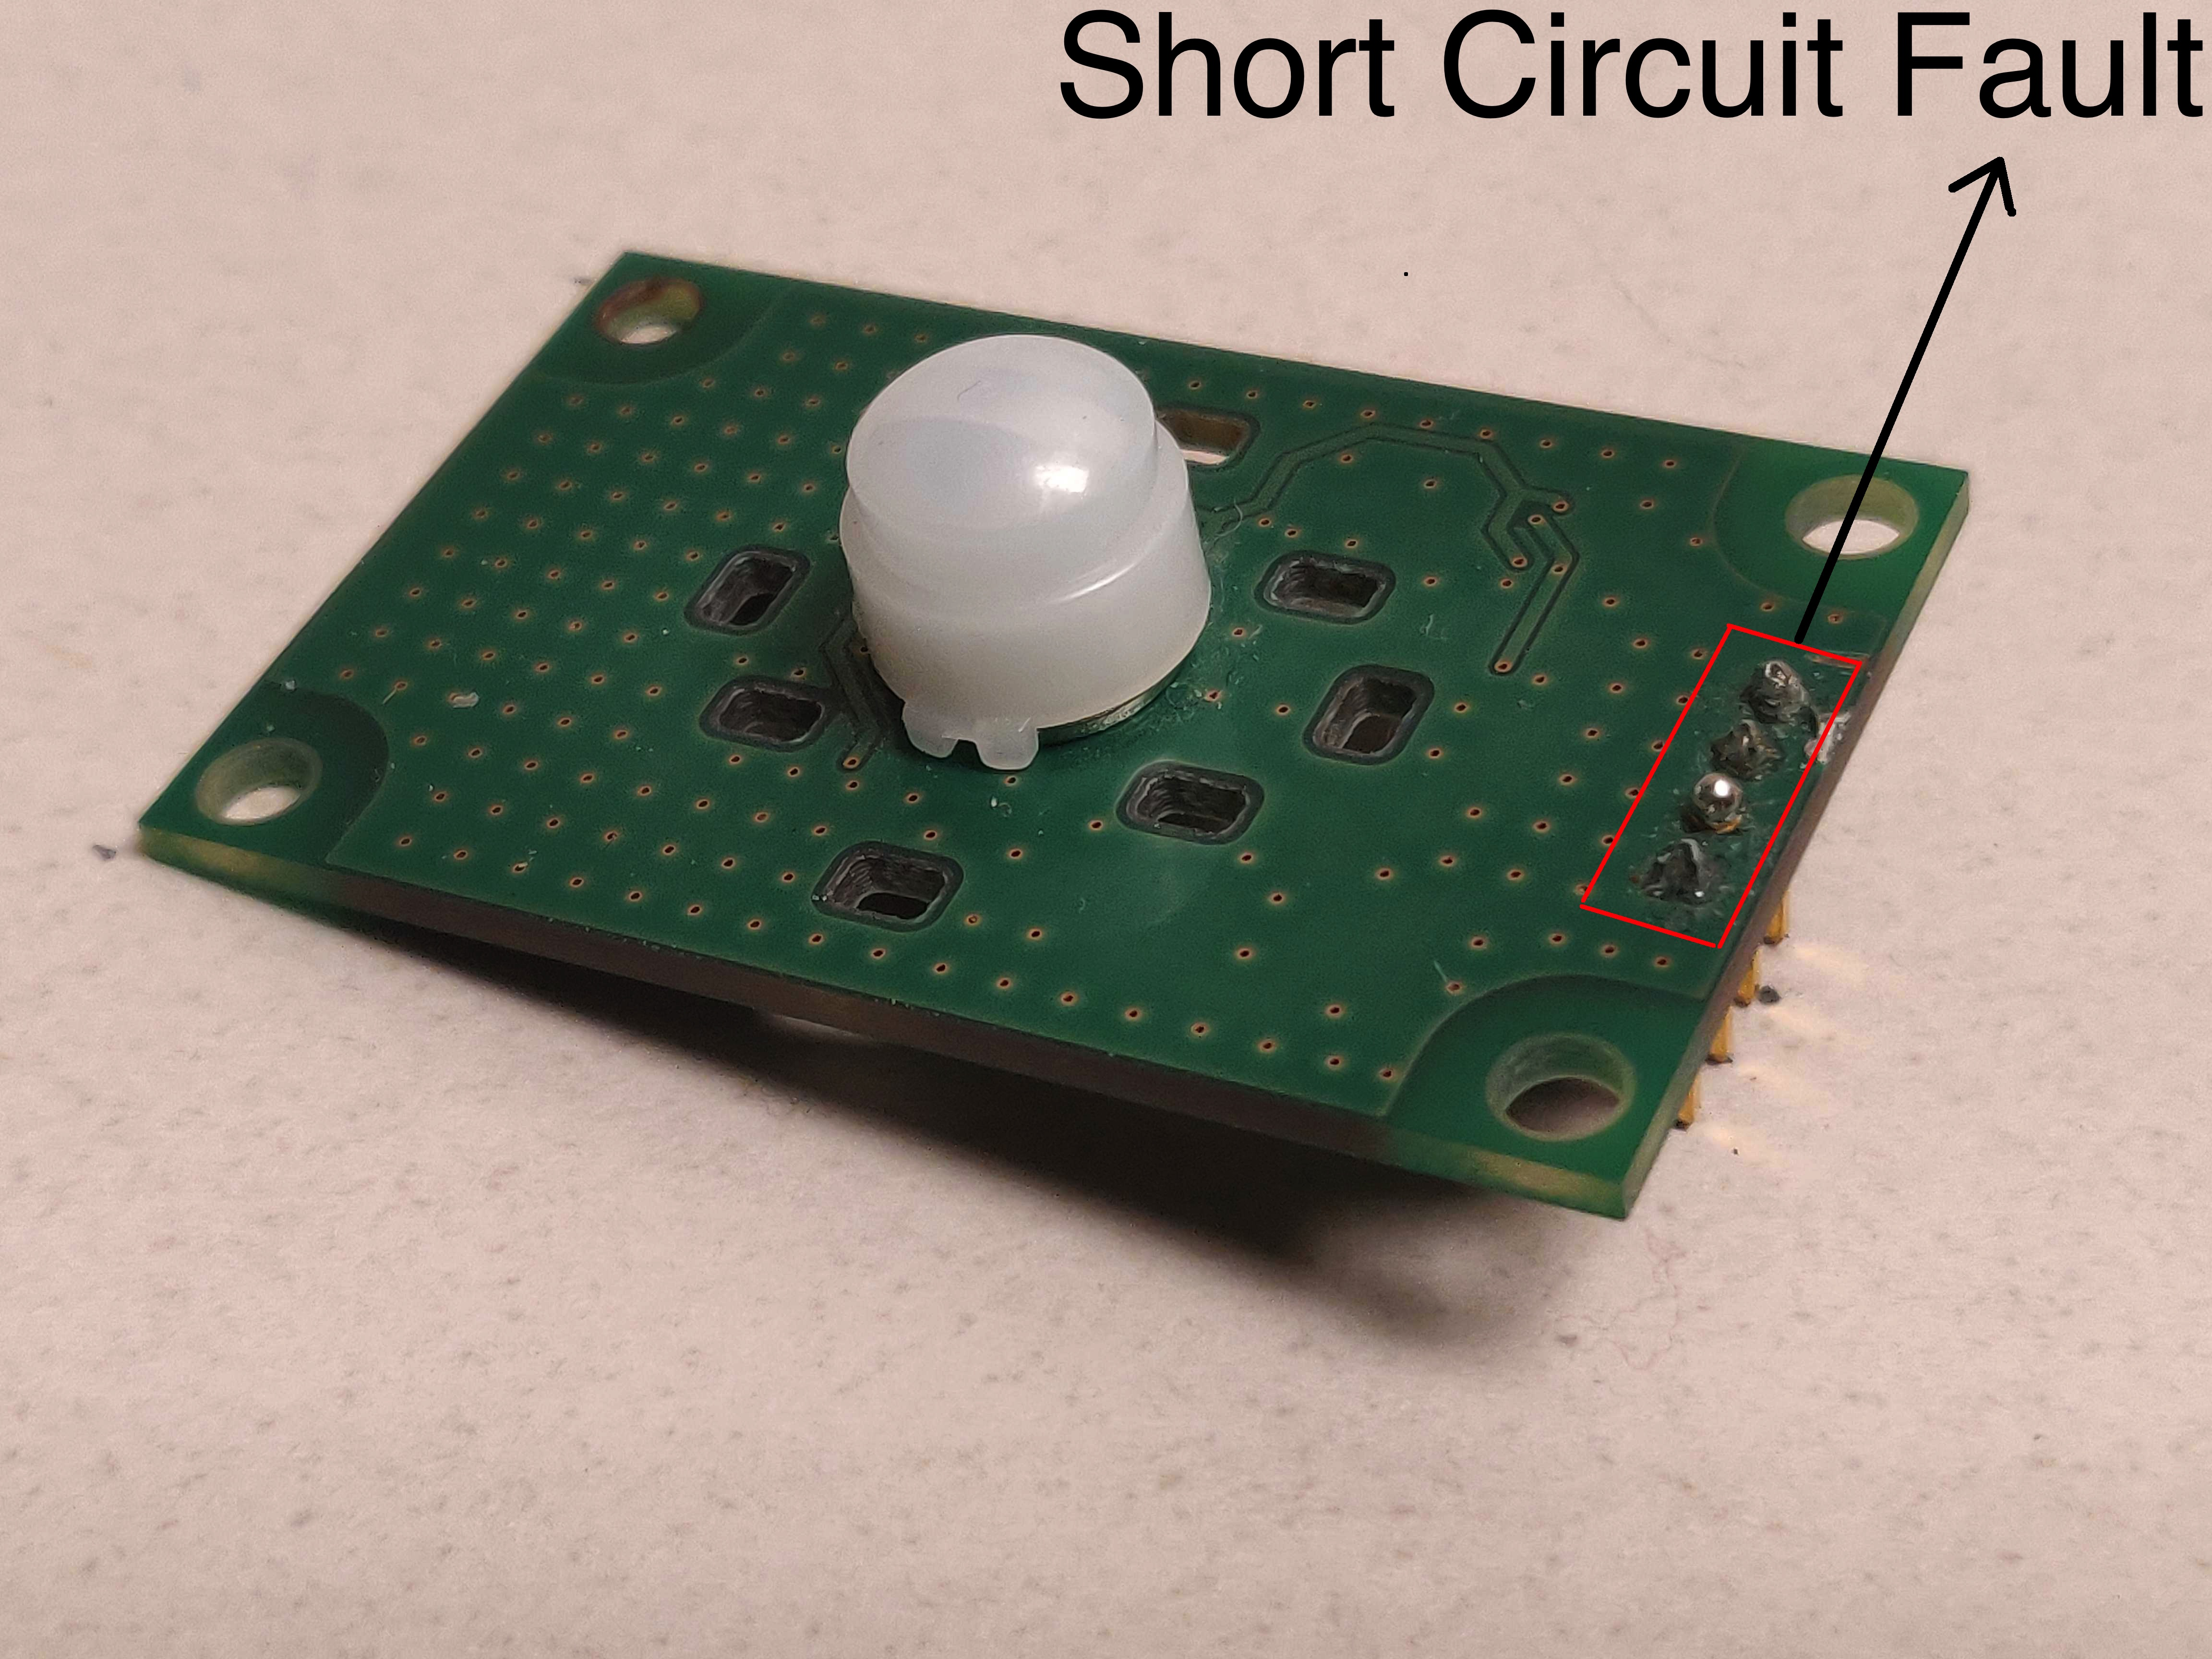
\includegraphics[width=\textwidth]{figures/platform/failure_photographs/ClassV-ElectronicsFault-annotated-jpg.jpg}
		\caption{Electronic Fault}
		\label{fig:failure_photo7}
	\end{subfigure}	
	\caption{\footnotesize{Some sensors} used in our study. Note that the failures are not always visually perceivable as the sensors are typically inaccessible.}
	\label{fig:pir_sensor_failure_photographs}
\end{figure}

\noindent \underline{Lens deformation (Class II):} As the lens is made of flexible, 0.4mm thick high density plastic~\cite{fresnel}, it is susceptible to deformation by physical damage. This can alter the curvature or puncture the lens. As in Class I, the consequence of failure is imperfect capture and focusing of the thermal radiation incident on the PIR sensor.

\noindent \underline{Lens hindrance (Class III):} Dust particles (\eg factory floors, building construction) or common objects such as paper and plastic tape can absorb the thermal radiation resulting in reduced to no radiation falling on the pyroelectric element. The deposition of particulate matter also causes dispersion.

In summary, Classes I--III failures affect the core functionality of the lens, and results in the imperfect capture and focus of thermal radiation.

\subsubsection{\textbf{Failures in the pyroelectric subsystem}: Optical Filter Damage (Class IV):} The optical filter and pyroelectric elements are prone to degradation with exposure to high temperature and humidity. As the optical filter is carefully calibrated to trigger in the region of human motion, it is susceptible to damage due to environmental factors such as heat sources (\eg room heaters, air-conditioners) and humidity (\eg oil condensation) as it affects the perceived temperature of the object. We name these as Class IV failures.

\subsubsection{\textbf{Failures in the Electronics}} On-board electronics consisting of filter, amplifier and comparator circuitry are prone to failures such as shorted or floating pins that we refer to as Class V failures. We only consider simple, electronic failures -- such as open, short circuits and floating inputs. Vendor-based IC testing procedures and board design process advancements have made electronic failures such as regulator, bus failures and PCB malfunctions infrequent in practice.


\noindent \textbf{Summary:} Failures in PIR sensors can occur in either the lens subsystem, the pyroelectric subsystem or the on-board electronics, each of which manifest differently in the underlying physics.

\begin{wraptable}{lr}{0.6\textwidth}\centering
	\footnotesize
	\caption{{\bfseries Taxonomy of Failures} in a PIR Sensor}
	\begin{tabular}{p{2.25cm} p{6cm}}
		\hline \textsc{\bfseries Failure} & \textsc{\bfseries Definition \& Impact}\\
		\hline\hline
		\rowcolor{gray!20} \multicolumn{2}{l}{\bfseries Lens Subsystem}\\
		Lens dislodged \newline (Class I) & Lens cap suffers partial or complete dislocation \eg physical impact with a foreign object, degradation of bonding,~\etc \\
		Lens deformed \newline (Class II) & Lens cap suffers physical damage in-place \eg deformation, puncture,~\etc \\
		Lens covered \newline (Class III) & Lens cap gets physically obstructed by foreign particles \eg dust, paper or tape \\
		\hline
		\rowcolor{gray!20} \multicolumn{2}{l}{\bfseries Pyroelectric Subsystem} \\
		Optical filter \newline damage (Class IV) & Damaged by environmental factors~\eg oil condensation\\
		\hline
		\rowcolor{gray!20} \multicolumn{2}{l}{\bfseries Electronic Subsystem} \\
		Electronic faults \newline (Class V) & Hardware failures~\eg short circuits, floating outputs~\etc \\
		\hline
	\end{tabular}
	\label{tab:pir_faults}
\end{wraptable}

\subsection{Analyzing Severity of Failures -- A Quantitative Analysis}
\label{subsec:quantify}
A failure is said to impact the sensor performance if the failure results in either false detections ({\bfseries FD}) \ie false positives or missed obstacles ({\bfseries MO}) \ie false negatives in the sensor output (\cout), compared to a working sensor. As seen in {\bfseries Fig.~\ref{fig:pir_sensor_different_lens}}, \cout is HIGH (1) when no is obstacle detected and \cout goes HIGH (1) $\rightarrow$ LOW (0) when an obstacle is detected.

\noindent \underline{Controlled Failure Study:} To understand the impact on sensor performance, in our lab, we take 2 PIR sensors, one which is without the fault (\working) and one with the fault (\tampered). The 2 sensors are placed in as close a proximity to one another as possible such that -- \ca distance between the sensors are closer than the size of obstacle, \cb the obstacle is moved in a plane such that it comes into the detection region of both the PIR sensors simultaneously. This implies that when the obstacle (we used our palm in this case) is moved across the detection region of both PIR sensors, it grazed both at the same time, triggering the same responses from both the sensors.

We then calculate the absolute difference ($\delta_N$) between the \cout values of the tampered sensor~\viz  \couttampered and the reference working sensor~\viz \coutworking by summing over all observations (Refer Eqn.~\ref{eqn:1}). Intuitively, a relatively low $\delta_N$ would imply that the tampered sensor is still in acceptable condition \ie the failure is not having much impact on the operation of the sensor. On the other hand, a high value of difference implies that the failure is much serious. To ease computation, we can also compute $\delta_N$ by dividing the time series into equal size chunks called \textit{windows} (W) and computing the difference between average \cout values of \tampered and \working in that window.

\begin{table}\small
	\centering
	\caption{\textbf{Misclassifications} analysis for different failures. The numbers indicate the deviation (as defined in Eqn.~\ref{eqn:1} between $C_{out}$ values) of a faulty sensor from that of a working sensor. Higher number indicates increased degree of failure.}
	\begin{tabular}{lllll}
		\hline
		\bfseries \textsc{Failure} & \bfseries \textsc{Lens Dislodged} & \bfseries \textsc{Lens Covered} & \bfseries \textsc{Heat Damage} & \bfseries \textsc{Humidity Damage}\\
		\hline \hline
		\rowcolor{gray!20} $\delta_N$$^1$ & 35 & 48 & 29 & 48 \\
		$\delta_N$$^2$ & 69 & 94  & 53 & 87 \\
		\hline 
	\end{tabular}
	\label{tbl:fault_degree}
	\quad \raggedright
	$^1$ 6 hour run, $^2$ 12 hour run
\end{table} 

\textbf{Table~\ref{tbl:fault_degree}} summarizes $\delta_N$ for a few types of failures as observed over 6-hour and 12-hour runs deployed in the elevator of our building. The numbers in the column represent deviation or misclassifications ($\delta_N$)~\ie the number of false detections (both false positives and false negatives) by the faulty sensor calculated using {\bfseries Eqn.~\ref{eqn:1}}.
We used a window size, $W$ = 1024 samples, which comes to a window of time duration slightly over 51 seconds at a sampling rate of 20 Hz.
In our case, the lens covered failure (8 failures per hour) is more pernicious than lens having fallen off (6 failures per hour).

\begin{equation}
	{\tikzmarknode{d}{\highlight{blue}{$\delta_N$}}} = \underset{windows}{\sum} 
	\left| {\tikzmarknode{t}{\highlight{red}{$C_{\text{out,tampered}}$}}} - {\tikzmarknode{w}{\highlight{green}{$C_{\text{out, working}}$}}}\right|,
	\label{eqn:1}
	\begin{tikzpicture}[overlay,remember picture,>=stealth,nodes={align=left,inner ysep=1pt},<-]
		\path (d.south) ++ (0,-0.6em) node[anchor=north east,color=blue!67] (scalep){\textbf{misclassifications}};
		\draw [color=blue!57](d.south) |- ([xshift=0.3ex,color=red]scalep.south west);
	\end{tikzpicture}
	\begin{tikzpicture}[overlay,remember picture,>=stealth,nodes={align=left,inner ysep=1pt},<-]
		\path (t.north) ++ (0,0.6em) node[anchor=south east,color=red!67] (scalep){\textbf{tampered}};
		\draw [color=red!57](t.north) |- ([xshift=-12ex,color=red]scalep.south east);
	\end{tikzpicture}
	\begin{tikzpicture}[overlay,remember picture,>=stealth,nodes={align=left,inner ysep=1pt},<-]
		\path (w.north) ++ (0,0.6em) node[anchor=south west,color=teal] (scalep){\textbf{working}};
		\draw [color=teal!57](w.north) |- ([xshift=-0.3ex,color=green]scalep.south east);
	\end{tikzpicture}
\end{equation}\\



\noindent \textbf{Summary:} Quantifying the impact of a failure gives hints on how pernicious specific failures are \textit{once they have been detected}.




\begin{figure}[b]
	\centering
	\begin{subfigure}[b]{0.3\textwidth}
		\centering
		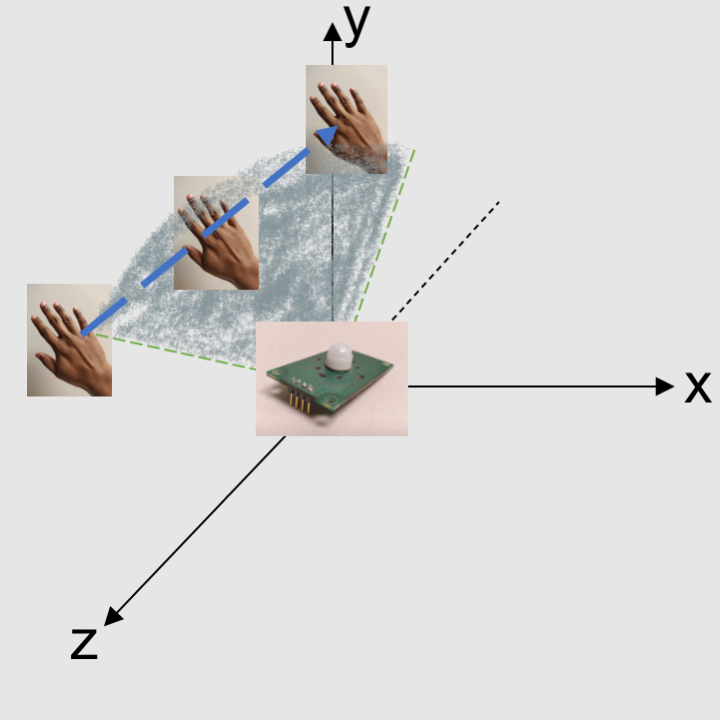
\includegraphics[scale=0.6, height=1.3in]{figures/platform/controlled_setup-2.png}
		\caption{Controlled Setup}
		\label{fig:pir_sensor_controlled}
	\end{subfigure}\begin{subfigure}[t]{0.3\textwidth}
		\centering
		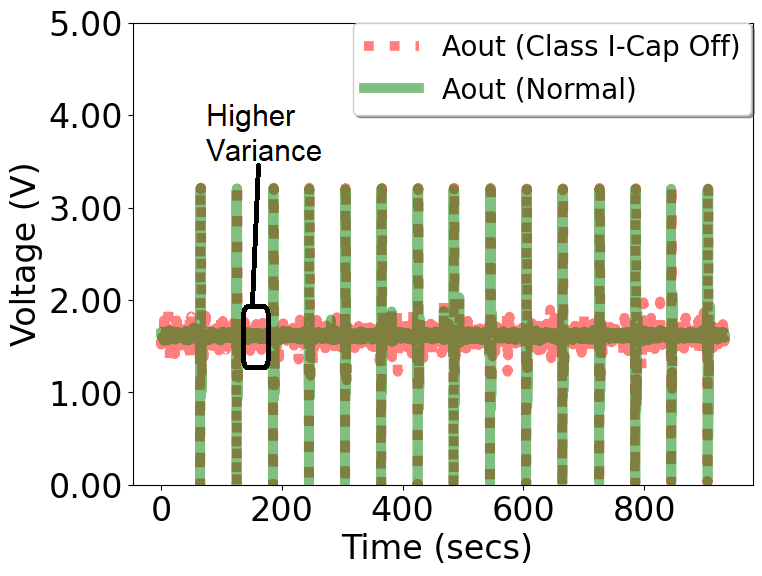
\includegraphics[width=\textwidth]{figures/2-PIR-Fault/normal-classI/classI_compared-again.png}
		\caption{Class I Fault}
		\label{fig:pir_sensor_controlled_a}
	\end{subfigure}\begin{subfigure}[t]{0.3\textwidth}
		\centering
		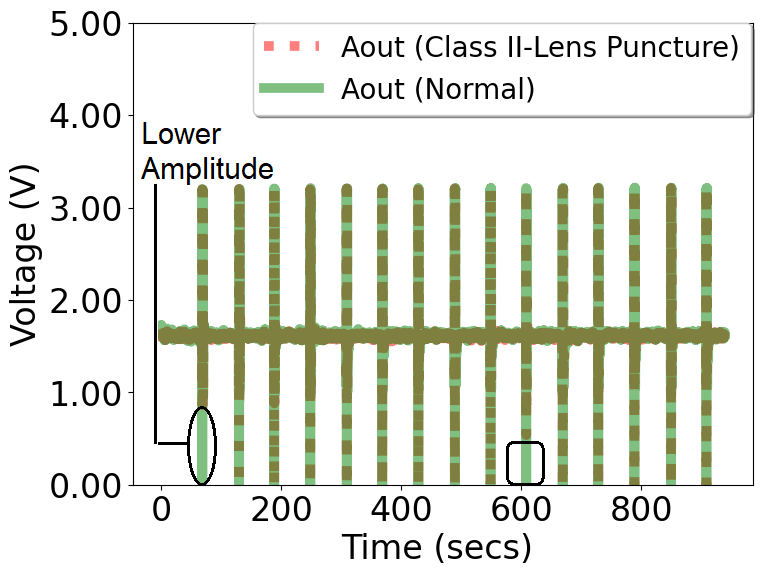
\includegraphics[width=\textwidth]{figures/2-PIR-Fault/normal-classII/classII_compared.png}
		\caption{Class II Fault}
		\label{fig:pir_sensor_controlled_b}
	\end{subfigure}\\\begin{subfigure}[t]{0.3\textwidth}
		\centering
		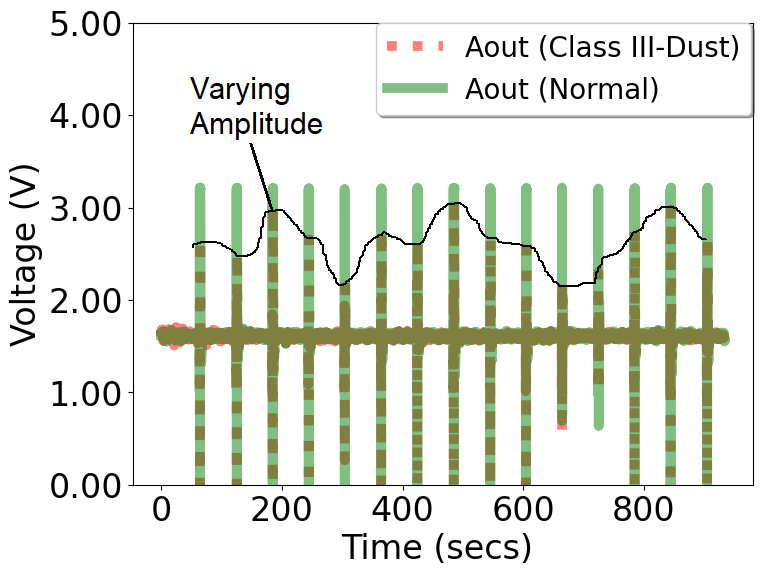
\includegraphics[width=\textwidth]{figures/2-PIR-Fault/normal-classIII/classIII_compared.png}
		\caption{Class III Fault}
		\label{fig:pir_sensor_controlled_c}
	\end{subfigure}
	\begin{subfigure}[t]{0.3\textwidth}
		\centering
		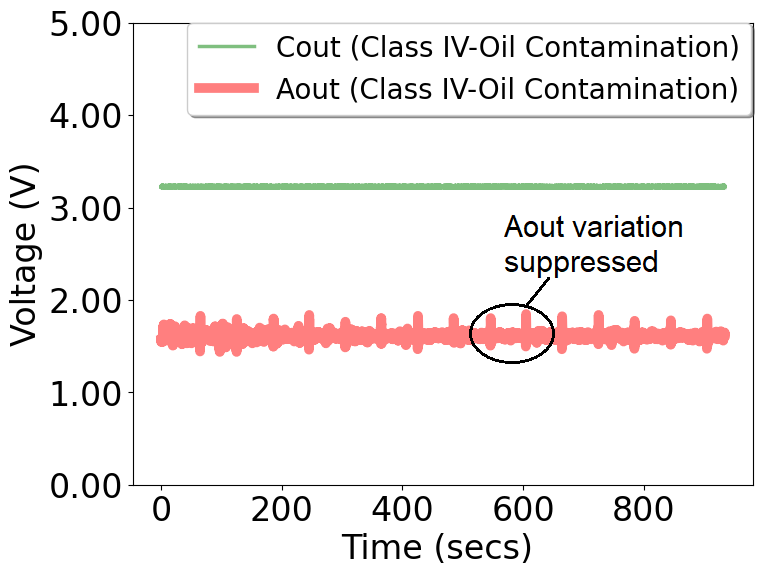
\includegraphics[width=\textwidth]{figures/2-PIR-Fault/normal-classIV/classIV_summary.png}
		\caption{Class IV Fault}
		\label{fig:pir_sensor_controlled_d}
	\end{subfigure}\begin{subfigure}[t]{0.3\textwidth}
		\centering
		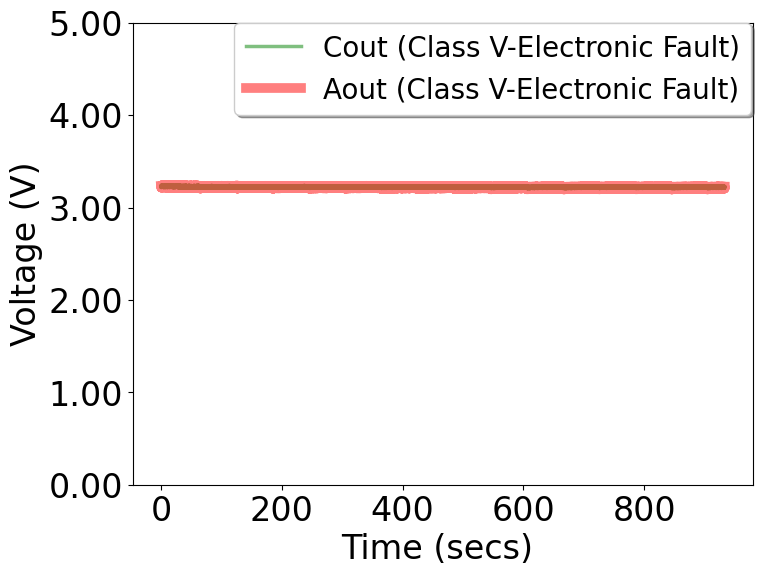
\includegraphics[width=\textwidth]{figures/2-PIR-Fault/normal-classV/classV_summary.png}
		\caption{Class V Fault}
		\label{fig:pir_sensor_controlled_e}
	\end{subfigure}
	\caption{(\ref{fig:pir_sensor_controlled_a} - \ref{fig:pir_sensor_controlled_e}) \footnotesize{\aout waveforms for sensor faults of Classes I--V}. Note that in Class I -- III faults, despite the obstacle still being detected, \aout provides indication of underlying abnormalities in the sensor.
	}
	\label{fig:pir_sensor_controlled_classI-V}
\end{figure}





 \section{Characterizing Failures using an Intrinsic Signal}
\label{sec:aout_char}
Our hypothesis is that the intermediate analog signal (\aout) from the pyroelectric element captures information that is critical to detect various failures. 
We now describe how this intrinsic signal and its underlying physics is useful to characterize failures.

\subsection{\aout signal to detect failures in PIR sensors}
\label{subsec:controlled}
As described in \S~\ref{subsec:working}, there are two output signals from a PIR sensor,~\viz \aout and \cout. 
The latter is a discrete signal typically used for detecting obstacle presence and is derived from \aout.
To show the utility of \aout, we conducted numerous controlled experiments where we manually injected commonly seen faults ({\bfseries Fig.~\ref{fig:pir_sensor_failure_photographs}}). 




Using the setup from {\S\ref{subsec:quantify}}, we co-located two sensors, \tampered and \working, where we change the \tampered sensor to test different types of failures described in \S\ref{subsec:taxonomy}. While in \S\ref{subsec:quantify}, we focused on \cout to study sensor performance during failure, in this experiment we additionally analyze \aout to get an understanding of the \textit{sensor physics} during failure.

We note the output signals (\ie \aout and \cout) from \tampered in every failure scenario and compare it with that from \working \emph{to understand the impact of failure on physics of the sensors}. Each experiment described below lasted for 15 minutes, where the obstacle (our palm in this case) was moved into the region of detection once every minute, as shown in {\bfseries Fig.~\ref{fig:pir_sensor_controlled}}. We plot \aout for both a working sensor and every type of faulty sensor in {\bfseries Figs.~\ref{fig:pir_sensor_controlled_a} --~\ref{fig:pir_sensor_controlled_e}}. The y-axis represents voltage output of \aout and x-axis represents time. For the working sensor \working, we expect a spike in \aout once every 60 seconds denoting motion of the palm. Let us now study the nature of \aout in each fault.

\textbf{Lens dislocation (Class I) faults.} The absence/dislocation of the lens causes imperfect focus of thermal radiation resulting in some residual output at the pyroelectric element even when there is no obstacle present. The impact of a Class I fault on \aout is shown in \textbf{Fig.~\ref{fig:pir_sensor_controlled_a}}. 
We can see that both the tampered and working sensors are still able to detect the obstacle (as shown by the 15 vertical spikes of \aout). However, when the obstacle is not present, we observe that the noise of \aout is much higher with a Class I fault as compared to a working sensor. Thus, it is important to look beyond just \cout signal to identify such failures.

\textbf{Lens deformation (Class II) faults.} Class II faults can potentially lead to missing obstacles at the periphery of the field of view due to deformation or loss of material integrity (\eg puncture). 
\textbf{Fig.~\ref{fig:pir_sensor_controlled_b}} shows the \aout for a sensor with a Class II fault. The amplitude of \aout at the times of obstacle detection is lower when compared to a working sensor. This is expected since the damage to lens leads to reduced thermal radiation incident on the pyroelectric subsystem. In general, Class II faults creates blind spots in the lens aperture that can reduce amplitude of the \aout signal. 


\textbf{Lens hindrance (Class III) faults} are caused due to foreign particles entering the lens that compromise its optical capability, thereby affecting the intensity and angle of radiation incident on the pyroelectric element. 
We induce such faults by depositing some dust on the lens.
\textbf{Fig.~\ref{fig:pir_sensor_controlled_c}} shows that the amplitude of \aout varies at each of the detection points. The variation depended on the amount of dust with respect to the orientation of the obstacle. Though the obstacle was still being detected, we note that with increased dust deposition, the amplitude of \aout can fall below the comparator threshold required to capture the obstacle, resulting in a missed obstacle \ie false negative. 




\textbf{Failure in pyroelectric components (Class IV).} Class IV faults happen when the optical filter on the pyroelectric element comes in contact with contaminants such as oil, mist or other smudge, resulting in potentially missing obstacles. High temperatures can also cause expansion of the optical filter that can also result in failures. 
We induce Class IV faults by spraying some oil on the optical filter. We observe in {\bfseries Fig~\ref{fig:pir_sensor_controlled_d}} that \aout has significantly attenuated spikes at each of the points that correspond to obstacle motion, but the spikes are not high enough to cause \cout to drop LOW. This results in the obstacle to be missed completely. A similar effect is observed when the optical filter is exposed to heat as it affects the temperature variation needed for pyroelectric effect.


\textbf{Failure in electronics (Class V) faults.} Class V faults are typically electronic faults such as short or open circuits. They can cause the \aout or \cout values to be `stuck' at certain anomalous value such as HIGH (3.3 V) or LOW (0 V). As a result, these failures can cause the obstacle to be completely missed. This is observed in {\bfseries Fig.~\ref{fig:pir_sensor_controlled_e}}, where \aout is shorted to the power supply, resulting in \cout following \aout and remaining HIGH. Consequently, the \aout waveform here is a flat, horizontal line and lacks oscillations. 

\noindent \textbf{Summary:} The core insight here is that \aout can shed light on the physical and electrical operating conditions of a PIR sensor as opposed to the mere boolean occupancy indicated by \cout. Thus, being able to snoop in on \aout can capture the interaction of IR radiation on the different sensor subsystems. 


\subsection{Analysis of \aout during partial failures and gradual degradation} \label{subsec:incremental_dust}In \S\ref{subsec:controlled}, we observed the impact of failures in PIR sensors, from classes I through V on nature of \aout and \cout. While we developed a structural taxonomy in \S\ref{subsec:taxonomy}, we note that failures need not be binary in nature, and there can be partial failures. Consequently, there are variations in each of the failure classes. For example, in Class III faults, the gradual build of dust can lead to degradation of sensing performance. \begin{figure*}[htbp]
	\centering
	\begin{subfigure}[t]{0.23\textwidth}
		\centering
		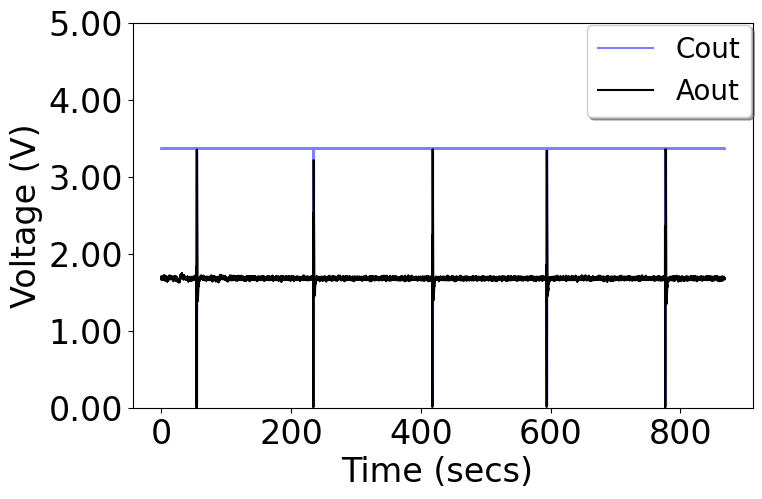
\includegraphics[width=\textwidth]{figures/gradual_degradation_dust/Stage0.png}
		\caption{Clean Sensor : Working}
		\label{fig:pir_sensor_classIII_fault_good}
	\end{subfigure}
	\hspace{1ex}
	\begin{subfigure}[t]{0.23\textwidth}
		\centering
		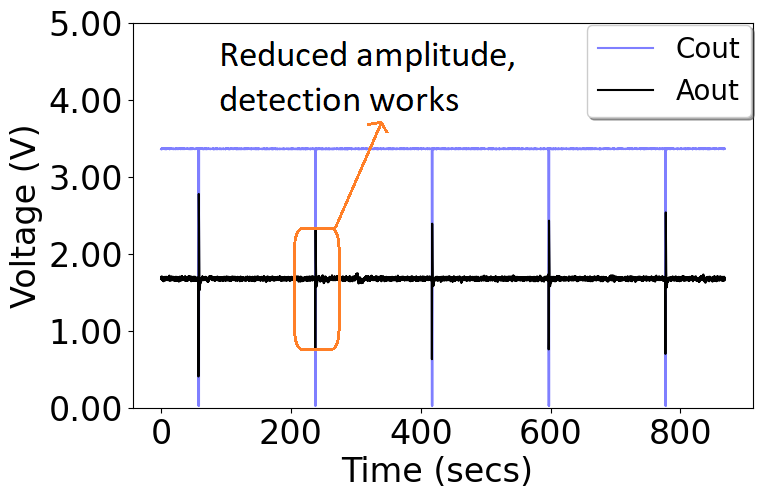
\includegraphics[width=\textwidth]{figures/gradual_degradation_dust/Stage1.png}
		\caption{Degraded Sensor : Still Working}
		\label{fig:pir_sensor_classIII_fault_bad1}
	\end{subfigure}	
	\hspace{1ex}
	\begin{subfigure}[t]{0.23\textwidth}
		\centering
		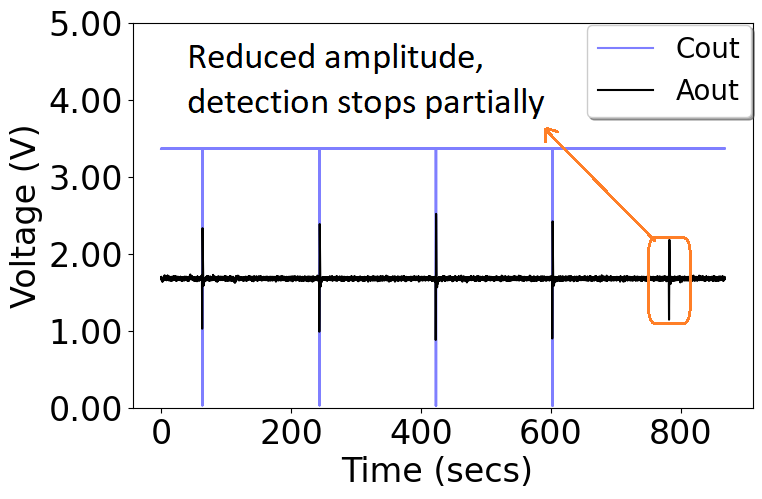
\includegraphics[width=\textwidth]{figures/gradual_degradation_dust/Stage2.png}
		\caption{Degraded Sensor : 1/5 miss}
		\label{fig:pir_sensor_classIII_fault_bad2}
	\end{subfigure}		
	\hspace{1ex}
	\begin{subfigure}[t]{0.23\textwidth}
		\centering
		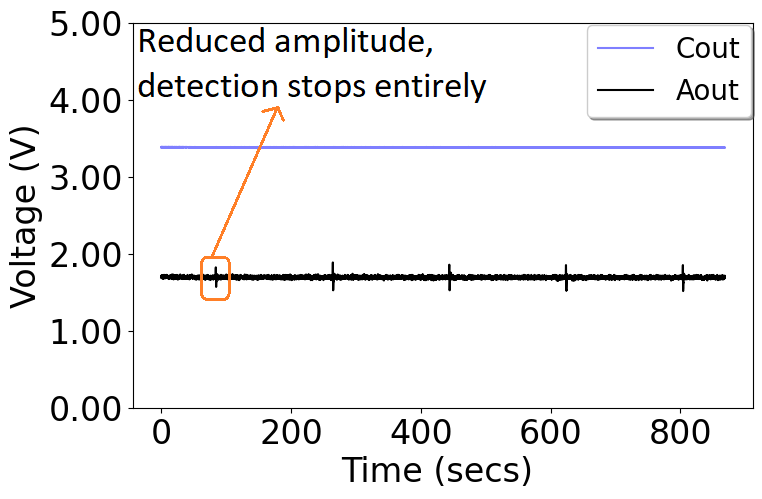
\includegraphics[width=\textwidth]{figures/gradual_degradation_dust/Stage3.png}
		\caption{Failed Sensor : 5/5 miss}
		\label{fig:pir_sensor_classIII_fault_bad3}
	\end{subfigure}	
	\caption{Dust gradually building up in different degrees causing Class III faults -- \ca is a clean sensor and dust gradually builds up \cb -- \cd at which stops detecting obstacles.}
	\label{fig:pir_sensor_classIII_fault_gradual}
\end{figure*}

To study the effect of gradual failures occurring in Class III, we divided a spatula of chalk-dust (approximately one-fourth of a teaspoon) and measured the effect of dust on response of the sensor. At every stage of study, we incrementally added dust and measured performance by plotting the two output signals \cout and \aout in the presence of an obstacle. The experiment is summarized in {\bfseries Fig.~\ref{fig:pir_sensor_classIII_fault_gradual}}. With increasing amount of dust being deposited, we see that the final discrete output misses the obstacle on occasion while detecting it sometimes. As a result, information about the dust deposition is lost at times from the final discrete output, \cout. \textit{Note that however, the intermediate analog output, \aout is able to capture information regarding the deposition of dust and by showing the degradation of sensing performance via its reduced amplitude.} Consequently, the obstacle detection process works till a reduced amplitude of \aout ({\bfseries Fig.~\ref{fig:pir_sensor_classIII_fault_good}} -- {\bfseries Fig.~\ref{fig:pir_sensor_classIII_fault_bad1}}), below which the sensor begins missing some obstacle instances ({\bfseries Fig.~\ref{fig:pir_sensor_classIII_fault_bad2}}). This process aggravates as more dust is accumulated on the sensor until a stage when there is a complete failure ({\bfseries Fig.~\ref{fig:pir_sensor_classIII_fault_bad3}}).

\noindent \textbf{Summary:} The key observation here is that capturing the physics of sensing via \aout helps glean valuable insights into even partial failures, which is completely absent in the \cout signal.


\subsection{Analysis of \aout during known quiet times} \label{subsec:aout_quiet_times} We draw some intuition on the behavior of \aout during known times of no occupancy, \eg post business hours in case of office buildings. The intuition stems from the arrangement of pyroelectric elements and its interplay with the lens subsystem. In a working sensor, we observe that due to the precise geometric arrangement of lens and pyroelectric elements, when there is no obstacle, the thermal radiation from the environment falls equally on the two pyroelectric elements, causing it to cancel out and leave very little noise at the output of pyroelectric subsystem. However, when the lens is covered by a foreign substance (\ie Class III fault), some of the thermal radiation is absorbed by the substance, before falling onto the pyroelectric elements. This results in a much lower noise at the output of pyroelectric subsystem. Alternately, if the lens is dislodged (\ie Class I fault), the two pyroelectric elements are not perfectly matched in differential configuration, which leads to higher noise at output of the pyroelectric subsystem. We observe this noise by measuring the \textit{noise floor} in the variance of \aout signal, during times of no obstacle.

Thus, we note that variance of \aout during a period with no occupancy can be used to get hints on Class I (lens dislodged) and Class III faults (lens covered). In particular, compared to a working sensor where the lens is mounted correctly, we expect a drop in variance when the lens is covered and a rise in variance when the lens is dislodged. In other words, $\sigma$(\aout)$|_{Class\ III}$ $\leq$ $\sigma$(\aout)$|_{Working}$ $\leq$ $\sigma$(\aout)$|_{Class\ I}$, where $\sigma$(\aout)$|_{X}$ denotes the variance of \aout under scenario X. We can use this idea to develop a preliminary fault detection algorithm that can be used to screen for lens faults (Class I and III). This requires computing two variance-based thresholds ($T_L$, $T_H$) to deduce status of the lens.
\begin{wrapfigure}{lr}{9.7cm}\centering
	\begin{subfigure}[t]{0.3\textwidth}
		\centering
		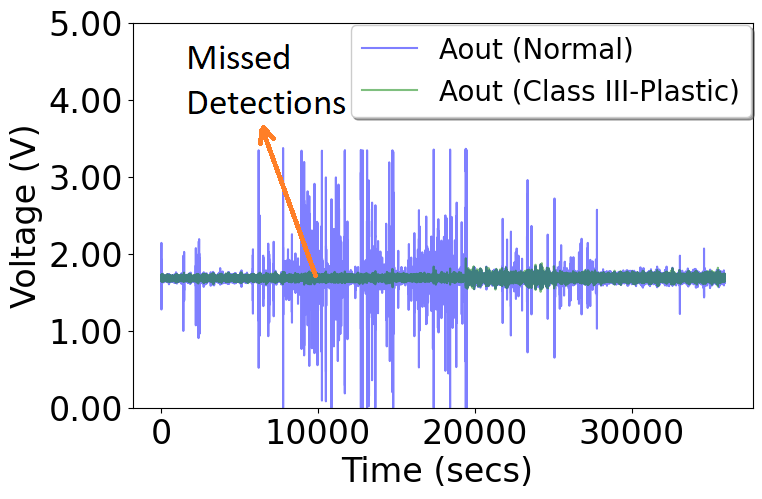
\includegraphics[width=\textwidth]{figures/2-PIR-Fault/normal-classIII/Aout_normal_vs_plastic.png}
		\caption{Plastic}
		\label{fig:pir_sensor_classIII_fault_plastic_tape}
	\end{subfigure}\hfill
	\begin{subfigure}[t]{0.3\textwidth}
		\centering
		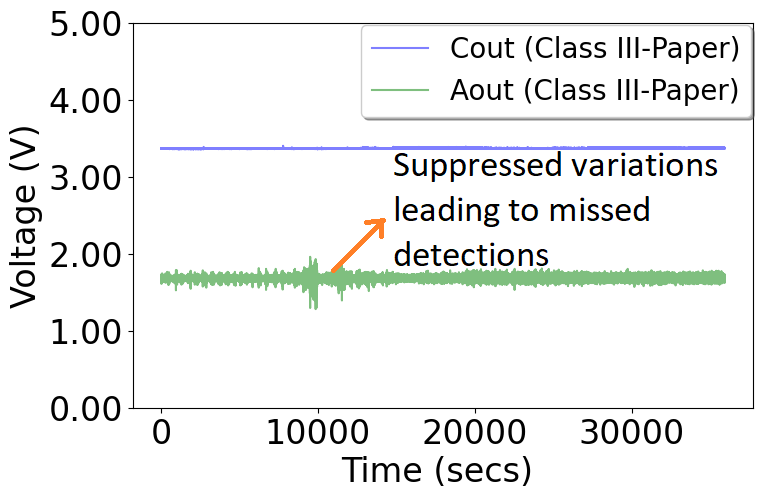
\includegraphics[width=\textwidth]{figures/2-PIR-Fault/normal-classIII/Cout_Aout_Paper.png}
		\caption{Paper}
		\label{fig:pir_sensor_classIII_fault_paper}
	\end{subfigure}	
	\caption{Effect of different foreign particles producing Class III faults of different degree -- the figures show that when the lens is obstructed with foreign particles like plastic tape and paper, it could result in complete failure.}
	\label{fig:pir_sensor_different_foreign_particles}
\end{wrapfigure}
However, we note that using the variance of \aout is not viable in all practical conditions. In particular, using this method works only during \textit{known quiet} times \ie in the known absence of occupancy which can be a \textit{disadvantage} for some deployments. As a result, this approach is suited for preliminary sensor health checks outside office or regular business hours of operation such as weekends. \\

\subsection{Analysis of different types of foreign particles} \label{subsec:foreign_additional}Different materials have distinct thermal characteristics and thus affect the \aout response differently in case of Class III faults. Stated alternately, the amplitude shaping of \aout varies depends on the material and its quantity. There are 3 kinds of foreign particles we study in our setup -- \ca paper, \cb plastic tape and \cc dust. We saw in {\bfseries Fig.~\ref{fig:pir_sensor_controlled_c}} how deposition of dust can compromise with the \aout responses. {\bfseries Fig.~\ref{fig:pir_sensor_different_foreign_particles}} shows Class III fault scenarios repeated with plastic tape and paper. In each of these runs, a normal sensor (represented in the blue curve in {\bfseries Fig.~\ref{fig:pir_sensor_classIII_fault_plastic_tape}}) detects obstacles as demonstrated by the \aout variation, whereas foreign particles such as plastic tape ({\bfseries Fig.~\ref{fig:pir_sensor_classIII_fault_plastic_tape}}) and paper ({\bfseries Fig.~\ref{fig:pir_sensor_classIII_fault_paper}}) can lead to a \textit{complete failure} of the PIR sensor.

\subsection{Frequency Domain Characterization} \label{subsec:freq_char} We have showed \aout signal has hints about various failure scenarios. To get additional insights, we transform the time domain \aout signal into frequency domain using the Fast Fourier transform (FFT) to derive robust features. FFT offers high resolution in the frequency domain and deconstructs the frequencies and harmonics present in a signal. Frequency domain representations have been used to characterize human activities using smartphone sensors and perform vibration screening for faults both in aircraft and railway lines~\cite{anguita2013public, HanlyWhy}.

We plot the FFT representations of \aout corresponding to different faults in {\bfseries Figs.~\ref{fig:classI_fault_freq}--~\ref{fig:classV_fault_freq}} as compared to a working sensor, all under the presence of an obstacle. The y-axis plots magnitude of FFT coefficients and the x-axis plots frequencies in the human range of motion (0 -- 10 Hz). In case of a working sensor, we observe 2 big peaks and additional peripheral frequencies up to 4 Hz. We now study how the frequency spectrum varies depending on the type of faults.

\textbf{Class I faults}  We observe in \textbf{Fig.~\ref{fig:classI_fault_freq}} that a dislodged lens cap (either partial or complete) leads to reduced information capture (lower bandwidth) and as a result, the sensitivity in the periphery of the sensors reduces. Note that there is just a single prominent peak in the faulty sensor (at a slightly lower frequency when compared to the normal sensor) that corresponds to the obstacle being perfectly aligned with the center of sensor as it passes. The magnitude reduces sharply as it moves away from the center of the sensor. 

\begin{figure}\centering
	\begin{subfigure}[t]{0.33\textwidth}
		\centering
		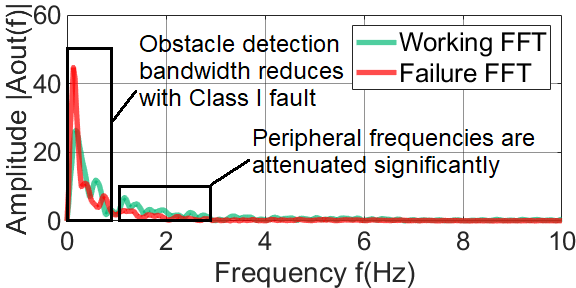
\includegraphics[width=\textwidth]{figures/2-PIR-Fault/normal-classI/class1_fft_coloradj_small_edited_camera_ready.png}
		\caption{Class I fault}
		\label{fig:classI_fault_freq}
	\end{subfigure}
	\begin{subfigure}[t]{0.33\textwidth}
		\centering
		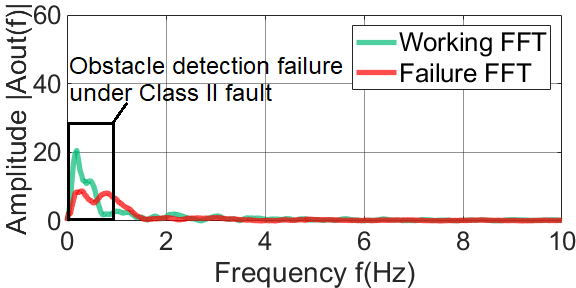
\includegraphics[width=\textwidth]{figures/2-PIR-Fault/normal-classII-deformed/class2_fft_coloradj_small_edited_camera_ready.png}
		\caption{Class II fault}
		\label{fig:classII_fault_freq}
	\end{subfigure}
	\begin{subfigure}[t]{0.325\textwidth}
		\centering
		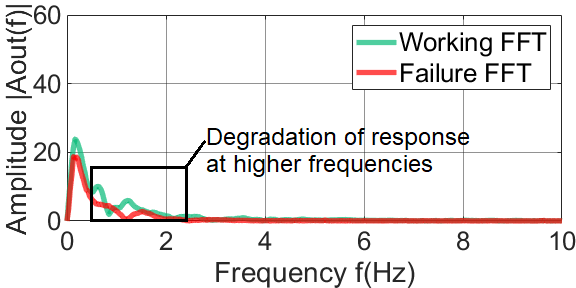
\includegraphics[width=\textwidth]{figures/2-PIR-Fault/normal-classIII/class3_fft_coloradj_small_edited_camera_ready.png}
		\caption{Class III fault}
		\label{fig:classIII_fault_freq}
	\end{subfigure}\\
	\begin{subfigure}[t]{0.33\linewidth}
		\centering
		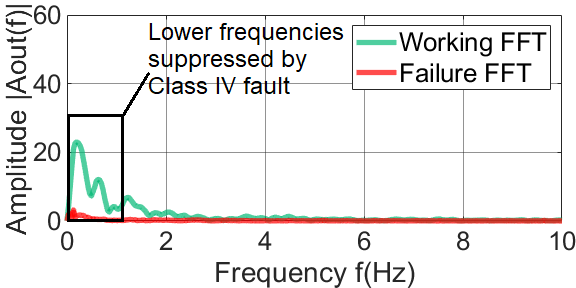
\includegraphics[width=\linewidth]{figures/2-PIR-Fault/normal-classIV/class4_fft_coloradj_small_edited_camera_ready.png}
		\caption{Class IV fault}
		\label{fig:classIV_fault_freq}
	\end{subfigure}
	\begin{subfigure}[t]{0.33\linewidth}
		\centering
		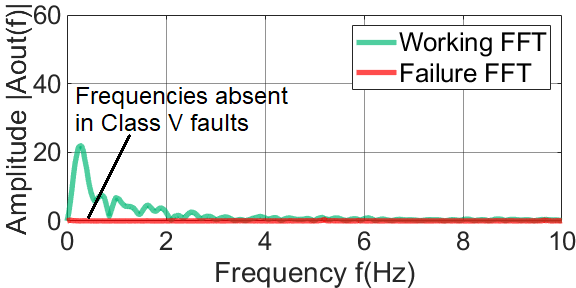
\includegraphics[width=\linewidth]{figures/2-PIR-Fault/normal-classV/class5_fft_coloradj_small_edited_camera_ready.png}
		\caption{Class V fault}
		\label{fig:classV_fault_freq}
	\end{subfigure}
	\begin{subfigure}[t]{0.325\linewidth}
		\centering
		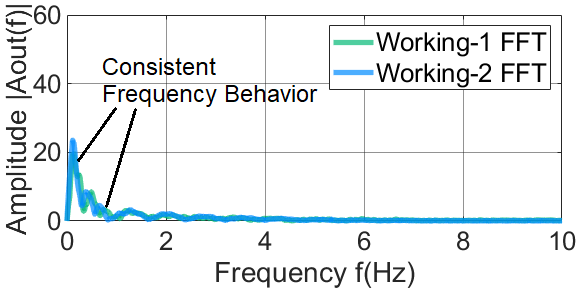
\includegraphics[width=\linewidth]{figures/2-PIR-Fault/normal-normal/normal_normal_fft_coloradj_small_edited_camera_ready.png}
		\caption{\textbf{Comparing} \aout of two working sensors}
		\label{fig:normal_normal_freq}
	\end{subfigure}
	\caption{\footnotesize{Frequency Domain Representations} of \aout under different faults in a PIR sensor. Only frequencies upto 10 Hz are shown as most PIR sensors detect human motion within 10 Hz.}
	\label{fig:classI-V_fault_freq}	
\end{figure}

\textbf{Class II faults} \textbf{Fig.~\ref{fig:classII_fault_freq}} plots the FFT for a sensor with deformed lens cap. 
We note that Class II faults lead to significantly suppressed primary peaks (approx. 10 db). In addition, the peripheral frequencies are attenuated as observed in Class I. These faults can manifest itself in reduced sensor performance as some of the detection region become \textit{blind spots} for the sensor.

\textbf{Class III faults} due to accumulation of foreign particles in the lens, lead to reduced sharpness of frequencies.
We observe in \textbf{Fig.~\ref{fig:classIII_fault_freq}} that the degradation starts with damping of the higher frequencies. As the amount of dust increases, we observe the frequencies getting increasingly damped until the object detection starts failing.

\textbf{Class IV faults}
We observe in \textbf{Fig.~\ref{fig:classIV_fault_freq}} that the frequencies present in the output are heavily suppressed resulting in missed obstacle detection. This is expected since the optical filter plays a major role in filtering out the non-human range frequencies from the thermal radiation and only passing through the frequencies corresponding to the human range. The presence of oil condensation or heat sinks causes absorption of the thermal radiation resulting in insufficient heat to cause pyroelectric effect. 

\textbf{Class V faults} such as open and short circuits are easy to detect due to the absence of any prominent frequencies. Consequently, \aout is \textit{stuck at} a value leading to only dc frequencies being present in the output. This result is observed in {\bfseries Fig.~\ref{fig:classV_fault_freq}}, where the \cout and \aout pins are shorted on the board. 

\noindent \textbf{Summary:} Frequencies present in FFT representations of \aout provide hints regarding status (\ie working/failed) of PIR sensors.





 \section{Fault Detection and Diagnosis} 
\label{sec:system_char}


In \S\ref{sec:aout_char}, we analyzed the impact of failures on the characteristics of the \aout output signal in both time domain and in frequency domain using FFT. We now investigate if the characteristics of \aout contain behavior that is amenable to learning \ie if there are features to be learnt. First, we analyze the learnability of the fault detection and diagnosis problem in \S\ref{subsec:learnability}. During this, we show that in every type of failure, there exists information about the failure and quantify the difference in physics captured by FFT coefficients using a K-S statistic test~\cite{massey1951kolmogorov}.

\begin{wraptable}{L}{0.4\textwidth}
	\setlength\tabcolsep{2.5pt}
	\centering
	\caption{{K-S Statistic Results}: FC1 -- FC5 : Failure Class I -- V. W : working sensor.}
		\begin{tabular}{l c c c c c c}
			\hline
			\textbf{Failure} & \textbf{FC1} & \textbf{FC2} & \textbf{FC3} & \textbf{FC4} & \textbf{FC5} & \textbf{W} \\
			\hline \hline
			K-S Test & 0.41 & 0.33 & 0.49 & 0.65 & 0.95 & 0.09 \\
			\hline 
		\end{tabular}
	\label{tbl:ks_test_results}
\end{wraptable}

\subsection{Learnability of the Analysis}
\label{subsec:learnability}

We performed a 2-sample Kolmogorov–Smirnov (K-S) statistic test~\cite{massey1951kolmogorov} to validate our hypothesis that the \aout distributions from both working and failed sensors are different.  We performed the tests at a significance level ($\alpha$) = 0.05, that results in a K-S statistic threshold of 0.1 -- a standard threshold for checking if sample differences in two distributions imply difference in population. {\bfseries Table~\ref{tbl:ks_test_results}} shows the K-S statistic (\texttt{kstest2} in Matlab~\cite{mathworks2015kstest2}) computed for each class of failure relative to a working sensor in columns FC1 -- FC5. We make the following observations :

\noindent \textbf{Failed sensors have different frequency characteristics compared to a working sensor:} Each failure class FC1 --- FC5 has a K-S statistic value > 0.1 when compared to a working sensor (W), indicating that the distributions of faulty and working sensors differ. 

\noindent \textbf{The worse the failure, higher the K-S statistic:} A sensor with oil condensation on the lens (C4) (a more pernicious fault leading to missed obstacles) resulted in a K-S statistic of 0.65 compared to 0.33 for a sensor with lens deformation (C2) (milder fault resulting in some blind spots). The K-S statistic captures the divergence between physics of failed and working sensors.


\noindent \textbf{Working sensors have similar characteristics:} We performed a sanity check between distributions of multiple working sensors and noticed the consistency among them in the frequency domain. Computing the K-S statistic resulted in a value below the 0.1 threshold implying similar physics as seen in {\bfseries Fig.~\ref{fig:normal_normal_freq}}.



\noindent \textbf{Summary:} K-S test shows the possibility of information that can be extracted to generate a physics-based reliability feature vector for the PIR sensor. This also motivates using classification techniques to identify the information difference between different failure scenarios~\cite{breiman2001random,cunningham2020k}.

\begin{figure}
    \begin{subfigure}[t]{0.45\textwidth}
		\centering
		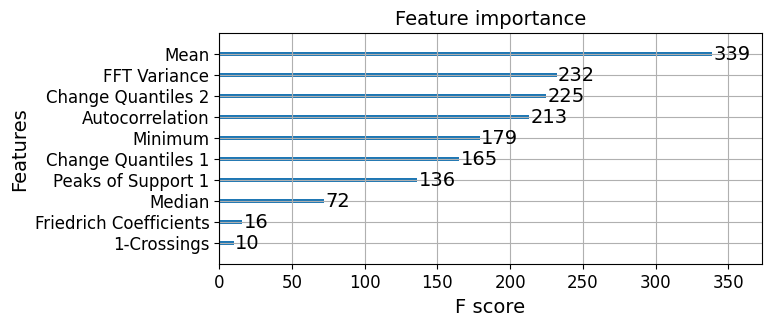
\includegraphics[width=\textwidth]{figures/classification/BH/BH-feature-selection.png}
        \caption{}
        \label{fig:BH_feature_selection}
    \end{subfigure}
    \hfill \begin{subfigure}[b]{0.49\textwidth}
        \centering
        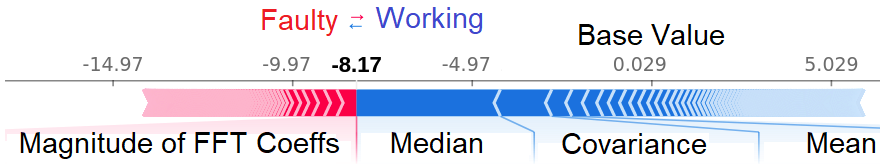
\includegraphics[width=\textwidth]{figures/classification/shapley/shap_expected_4.png}
        \caption{}
        \label{fig:shapley_summary}
    \end{subfigure}
    \caption{\ca Top 10 features selected using B-H procedure, \cb Summary of Shapley Values showing FFT coefficients separate faulty and working classes.}
\end{figure}

\subsection{Feature Selection and Importance} 
\label{subsec:bh} 
We use both the time domain and frequency domain features of the \aout signal to classify the sensor to either working or one of the faulty classes. As the number of features that can be derived is huge (\eg in our case 305), we use the Benjamini-Hochberg (B-H) feature selection algorithm ~\cite{benjamini1995controlling} to estimate and analyze \textit{feature importance} in the \aout collected for working and each class of faulty sensors.

B-H technique is used offline with training data to decide which features are useful in predicting the label of the sensor (\eg working vs. class X). The output of B-H feature selection process is a \textit{feature importance score (F-score)} that indicates how useful or valuable each feature is in the decision making process. The higher the F-score, the more important the feature is to prediction. 

B-H feature selection process works by initially training an ensemble of decision trees on all features, derived from both time and frequency domain features as mentioned in Christ~\etal~\cite{christ2018time} and implemented in the open source library \texttt{tsfresh}~\cite{tsfresh2018code}. It then measures the prediction accuracy using every feature. This gives a high accuracy at the expense of overfitting. Thereafter, each feature vector is independently evaluated with respect to its significance for prediction using hypothesis testing, assigning it a F-score. It then iteratively prunes features having low F-scores, trains decision trees using these reduced features and measures prediction accuracy. The process stops when a user-set threshold of accuracy is met or when all the combinations have been tested. 

Applying the B-H process to our training data containing both faulty and working sensors, \emph{we pruned 305 features for our entire data set to obtain 10 features at a slightly better accuracy}. The larger set of features are derived from the list of features in {\bfseries Table~\ref{tbl:feat_list}}. \texttt{tsfresh} attempts to identify the strongly and weakly-relevant features in the fault detection and diagnosis process. It uses an algorithm named \texttt{fresh} (`FeatuRe Extraction based on Scalable Hypothesis'), that has been shown to be an efficient, scalable feature extraction technique used in early stages of ML pipelines~\cite{christ2016distributed, christ2018time}. \texttt{fresh} uses a 3-phase technique to select significant features while controlling the percentage of irrelevant features. First, \texttt{fresh} characterizes the time series using the larger set of features, some of which are indicated in {\bfseries Table~\ref{tbl:feat_list}}. Note that the complete feature set is comprehensive and also includes composite features derived from the simple features. In the second step, each feature vector is individually and independently evaluated with respect to its significance using hypothesis testing. As a part of the hypothesis testing, the significance of each feature is quantified into a p-value, with smaller p-values indicating that the feature is not statistically significant. In the third and last step, the feature vector is evaluated using the B-H process to decide which features to keep -- by transforming the hypothesis testing scores into F-scores. This step ensures that incorrectly rejected features are regulated while conducting multiple hypothesis tests. {\bfseries Fig.~\ref{fig:BH_feature_selection}} plots the F-score for the selected 10 key features in both time and frequency domains. These include: \ca FFT Variance that indicates how spread the frequency distribution is, \cb Autocorrelation that generalizes periodicity or patterns in the time domain, and \cc  Measures of central tendency such as mean, median and change quantiles that measure the time domain changes within a corridor. This process is performed offline and the significance of the pruned feature set is guaranteed by the B-H algorithm. Note that both Friedrich coefficients and Peaks of support capture short term dynamics of the signal. The mathematical definition of these features can be found in statistics textbooks and implementations in the \texttt{tsfresh} GitHub repository~\cite{tsfresh2018code}. We can continue the feature pruning process by training decision trees on combinations of features from these 10 features and measuring prediction accuracy. We stopped the feature pruning with 10 features since we consistently obtained an accuracy of 97-99\% in practice with this smaller set of features.


\begin{table}
	\centering
	\footnotesize
    \caption{Features before pruning, calculated using the \texttt{tsfresh}~\cite{tsfresh2018code} library. \texttt{tsfresh} uses hypothesis testing to prune and select most significant features.}
    \begin{tabular}{p{2.25cm} p{12 cm}}
    \hline \textsc{\bfseries Feature} & \textsc{\bfseries Description}\\
    \hline\hline
    \rowcolor{gray!20} abs\_energy & Absolute energy \ie sum of squares   \\
    agg\_autocorrelation & autocorrelation of the time series \\
    \rowcolor{gray!20} agg\_linear\_trend & linear least-squares regression aggregated over chunks versus the sequence from 0 up to (number of chunks - 1) \\
    approximate\_entropy & vectorized approximate entropy \\
    \rowcolor{gray!20} c3 & c3 statistics to measure non linearity \\
    binned\_entropy & calculates entropy over a set of equidistant bins \\
    \rowcolor{gray!20} energy\_ratio\_by\_chunks & the sum of squares of chunk expressed as a ratio with the sum of squares over the whole series \\
    fft\_aggregated & the spectral centroid (mean), variance, skew, and kurtosis of the absolute fourier transform spectrum \\
    \rowcolor{gray!20} fft\_coefficient & the fourier coefficients of the one-dimensional discrete fourier transform \\
    fourier\_entropy & the binned entropy of the power spectral density of the series \\
    \rowcolor{gray!20} friedrich\_coefficients & Coefficients of polynomial fitted to the Langevin model \\
    linear\_trend & a linear least-squares regression for the values of the series versus the sequence from 0 to length of the time series minus one \\
     \rowcolor{gray!20} number\_peaks & the number of peaks of at least support n \\
    root\_mean\_square & the root mean square (rms) of the series \\
     \rowcolor{gray!20} number\_crossing\_m & the number of crossings of series across m \\
    sample\_entropy & sample entropy of the series \\
     \rowcolor{gray!20} variation\_coefficient & the variation coefficient (standard error / mean, give relative value of variation around mean) of the series \\
    ratio\_beyond\_r\_sigma & ratio of values that are more than $r$ standard deviations away from the mean \\
     \rowcolor{gray!20} others & mean, variance, quantile, mean absolute change and so on \\
    \hline
    \hline
    \end{tabular}
    \label{tbl:feat_list}
\end{table}





\subsection{Monitoring Feature Performance using Shapley Additive Explanations (SHAP)} \label{subsec:shap} Once the important features are identified using the B-H feature selection process, we use the technique of SHAP~\cite{NIPS2017_8a20a862} values to \textit{explain or interpret} the output of a prediction. SHAP uses game-theoretic techniques to explain how the output of a prediction changes by conditioning on every feature present in the reduced feature set given by B-H process.  




{\bfseries Fig.~\ref{fig:shapley_summary}} shows an example of how SHAP values are analyzed for a particular prediction on a classification between faulty and working sensors. The features in red contribute to the sensor being predicted as faulty, whereas the features in blue contribute to the sensor being predicted as working. As seen, the competing features that contributed to this decision are the FFT coefficients and the statistical features~\viz mean, median and covariance. 
In this prediction, the FFT coefficients push the prediction to that of a faulty sensor while the mean, median and covariance push the prediction to a working sensor. The base value is the average SHAP value output by the model for the entire training dataset, and the value in bold is the SHAP value for this particular prediction. We leverage an open-source library implementation of the algorithm from Lundberg~\etal~\cite{NIPS2017_8a20a862, shap_implementation} that sorts the features by sum of SHAP value magnitudes over all the samples and conditionally rejects the feature contributing lowest to the prediction. Thus, we use the feature explanations from SHAP values to tune the model performance. 

\subsection{\sol: Fault Detection \& Analysis Algorithm}
\label{subsec:high_level_algorithm}
We now combine the insights gathered from physics and machine learning techniques to develop a unified algorithm, called \sol, that is deployable at the edge, to isolate and diagnose faults.
\sol consists of 2 stages: \ci pre-deployment (training) stage, wherein the reference \aout values for a set of sensors (both working and faulty) are collected offline and analyzed to extract key features and \cii deployment stage, wherein the features from a operational \aout signal is matched with the previously extracted features in order to detect and isolate faults. We next describe both the stages in detail.

\begin{figure}\noindent
	\begin{minipage}[t]{0.26\textwidth}
		\centering
		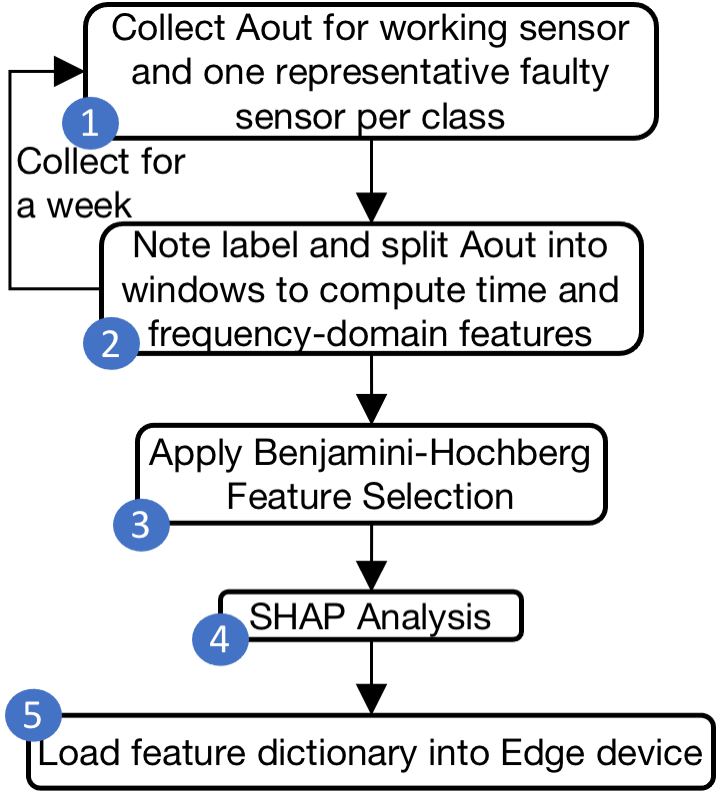
\includegraphics[width=0.9\textwidth]{figures/deployment/predeployment-stage-2.png}
		\caption{\footnotesize{Pre-deployment stage}.}
		\label{fig:pre_deployment_steps}
	\end{minipage}\begin{minipage}[t]{0.22\textwidth}
		\centering
		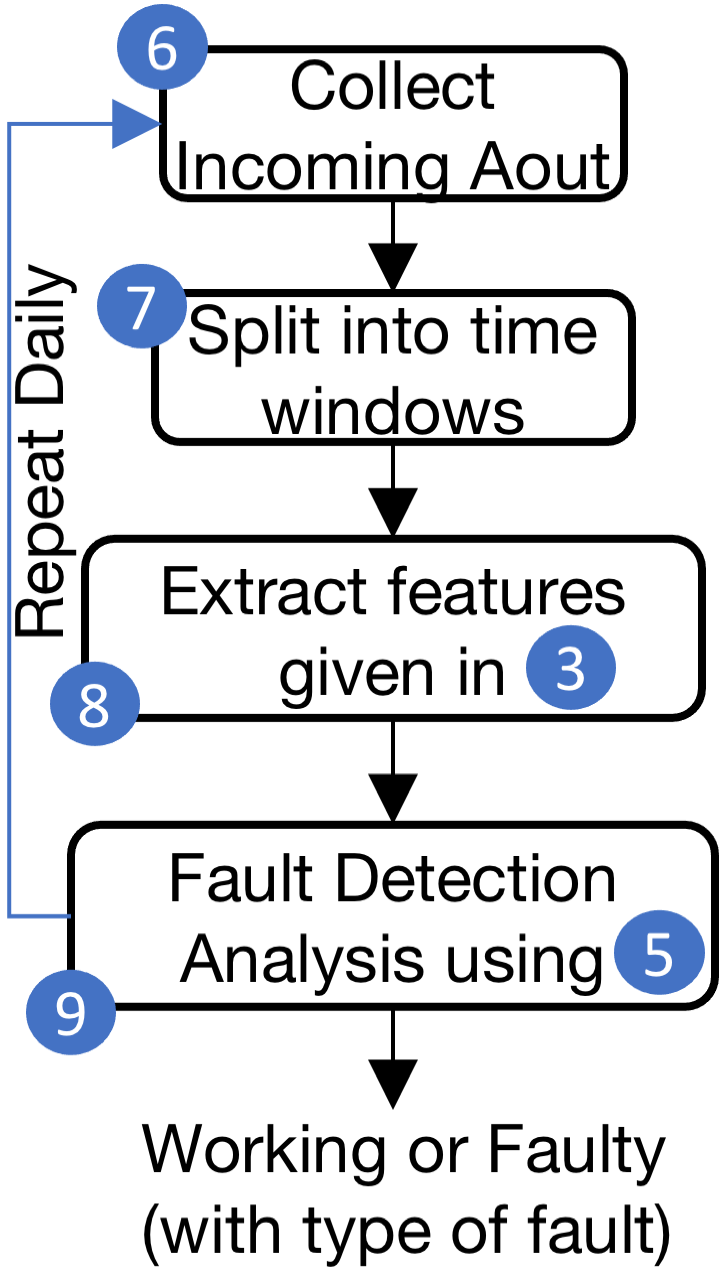
\includegraphics[width=0.7\textwidth]{figures/deployment/deployment-stage-5.png}
		\caption{\footnotesize{Deployment stage}.}
		\label{fig:deployment_steps}
	\end{minipage}\begin{minipage}[b]{0.48\textwidth}
		\centering
		\footnotesize
		\captionof{table}{Details of Evaluation Setup used in \sol}
		\begin{tabular}{p{2.6cm} p{4.1cm}}
			\hline \textsc{\bfseries Component} & \textsc{\bfseries Specifications \& Details}\\
			\hline\hline
			\rowcolor{gray!20} \multicolumn{2}{l}{\bfseries Data Collection \& Analysis Platform}\\
			Arduino Mega 2560 Rev3 & ATmega2560 16 MHz with 256 kB Flash \\
			Raspberry Pi v3.0 Model B & Quad Core 1.2GHz Broadcom BCM2837 64bit CPU, 1GB RAM \\
			\hline
			\rowcolor{gray!20} \multicolumn{2}{l}{\bfseries Connectivity \& Power} \\
			USB Serial Cable & Interface between Raspberry Pi and Arduino Microcontroller\\
			Power Supply & 5V for Arduino and 3.3V for Raspberry Pi\\
			\hline
			\rowcolor{gray!20} \multicolumn{2}{l}{\bfseries Sensor} \\
			PIR Sensor & Murata PIR Evaluation Board IMX-060 \\
			\hline
		\end{tabular}
		\label{tab:pir_platform}
	\end{minipage}
\end{figure}




\subsubsection{Pre-deployment stage} 
\label{sebsec:pre_deploy} 
We first collect \aout from a set of sensors, comprising both working and faulty ones such as the ones shown in {\bfseries Fig.~\ref{fig:pir_sensor_failure_photographs}}. The collected time series data are labeled to form a training dataset. We perform the Benjamini-Hochberg (B-H) feature selection on this dataset to extract key features such as FFT coefficients of \aout for each class of sensor. This forms a feature dictionary containing a smaller number of features along with the failure as a label. We further verify the importance of these features using SHAP analysis and refine the features if necessary.
We then build a classifier model to uniquely identify the sensor failure and load this model into the edge device connected to the PIR sensor. 

We now describe the steps involved ({\bfseries Fig.~\ref{fig:pre_deployment_steps}}):
\circled{1} We deploy the working and faulty sensors for a short duration (say few days) in a real-world environment to collect realistic \aout signals for low, medium and high occupancy. 
Note that this is a one-time activity performed for a specific PIR sensor type/manufacturer. 
We used 15 sensors comprising a mix of working and faulty sensors capturing failures in each class as our training set.
\circled{2} We note the label of a sensor and split the \aout values into equal-sized time slices (windows) to calculate different time and frequency-domain features. 
\circled{3} We apply B-H feature selection process for each type of sensor to identify unique and key features. 
\circled{4} We performed SHAP analysis to understand the performance of each feature towards classification and refine them accordingly. 
\circled{5} We use the final set of features along with class labels to build a classifier model (we use random forest as our classifier model). This model is then loaded onto the edge devices for fault detection and analysis. We note that while \circled{2} and \circled{3} are computationally expensive, it is acceptable as it is performed offline only once in the pre-deployment.

\subsubsection{Deployment stage} 
This stage consists of the following steps ({\bfseries Fig.~\ref{fig:deployment_steps}}): 
\circled{6} First, the operational \aout output signals for the deployed sensors are collected. 
\circled{7} We split the \aout into equal-sized windows using same window size as in the pre-deployment. 
\circled{8} We extract the necessary features from the \aout signal. 
\circled{9} We use a classifier to \ca isolate faulty from working sensors and \cb identify the class of failure in the faulty sensor if applicable. The fault detection (steps \circled{6} - \circled{9}) depends on the application requirements, \ie every hour, day or week. 







 \section{Implementation}
\label{sec:impl}

Our solution is designed using commodity off the shelf (COTS) components.
The open-source implementation\footnote{Available at: \url{https://github.com/synercys/PIRMedic}} includes:

\ca \textbf{Edge Hardware} consisting of -- \ci a PIR sensor~\cite{PIR_sensor_eval}, \cii a bare-metal platform~\viz Arduino Mega Microcontroller Unit (MCU)~\cite{arduino_mega} 
for sensor data capture, and \ciii a Linux-based platform~\viz Raspberry Pi~\cite{rpi3} 
for executing the fault detection and diagnosis algorithm, \sol. The specifications of hardware used can be seen in {\bfseries Table~\ref{tab:pir_platform}}.

The Arduino MCU polls the sensor hardware signals (\ie \cout and \aout) periodically over a GPIO interface. We poll the PIR sensors at a frequency $\geq$ 20 Hz due to the \textit{Nyquist criterion} as the human motion information in the PIR sensor is between 0 -- 10 Hz. Note that using a bare-metal platform allows us to capture \aout samples at a constant rate. The Raspberry Pi platform performs the fault detection and analysis for the data captured at the Arduino MCU.
The Raspberry Pi and Arduino are connected via a Micro-USB cable and the data captured at the Arduino MCU is serially transferred to the Raspberry Pi for analysis, as shown in {\bfseries Fig.~\ref{fig:eval_platform}}.

\begin{figure}
	\begin{minipage}[t][4 cm][c]{0.28\textwidth}
		\centering
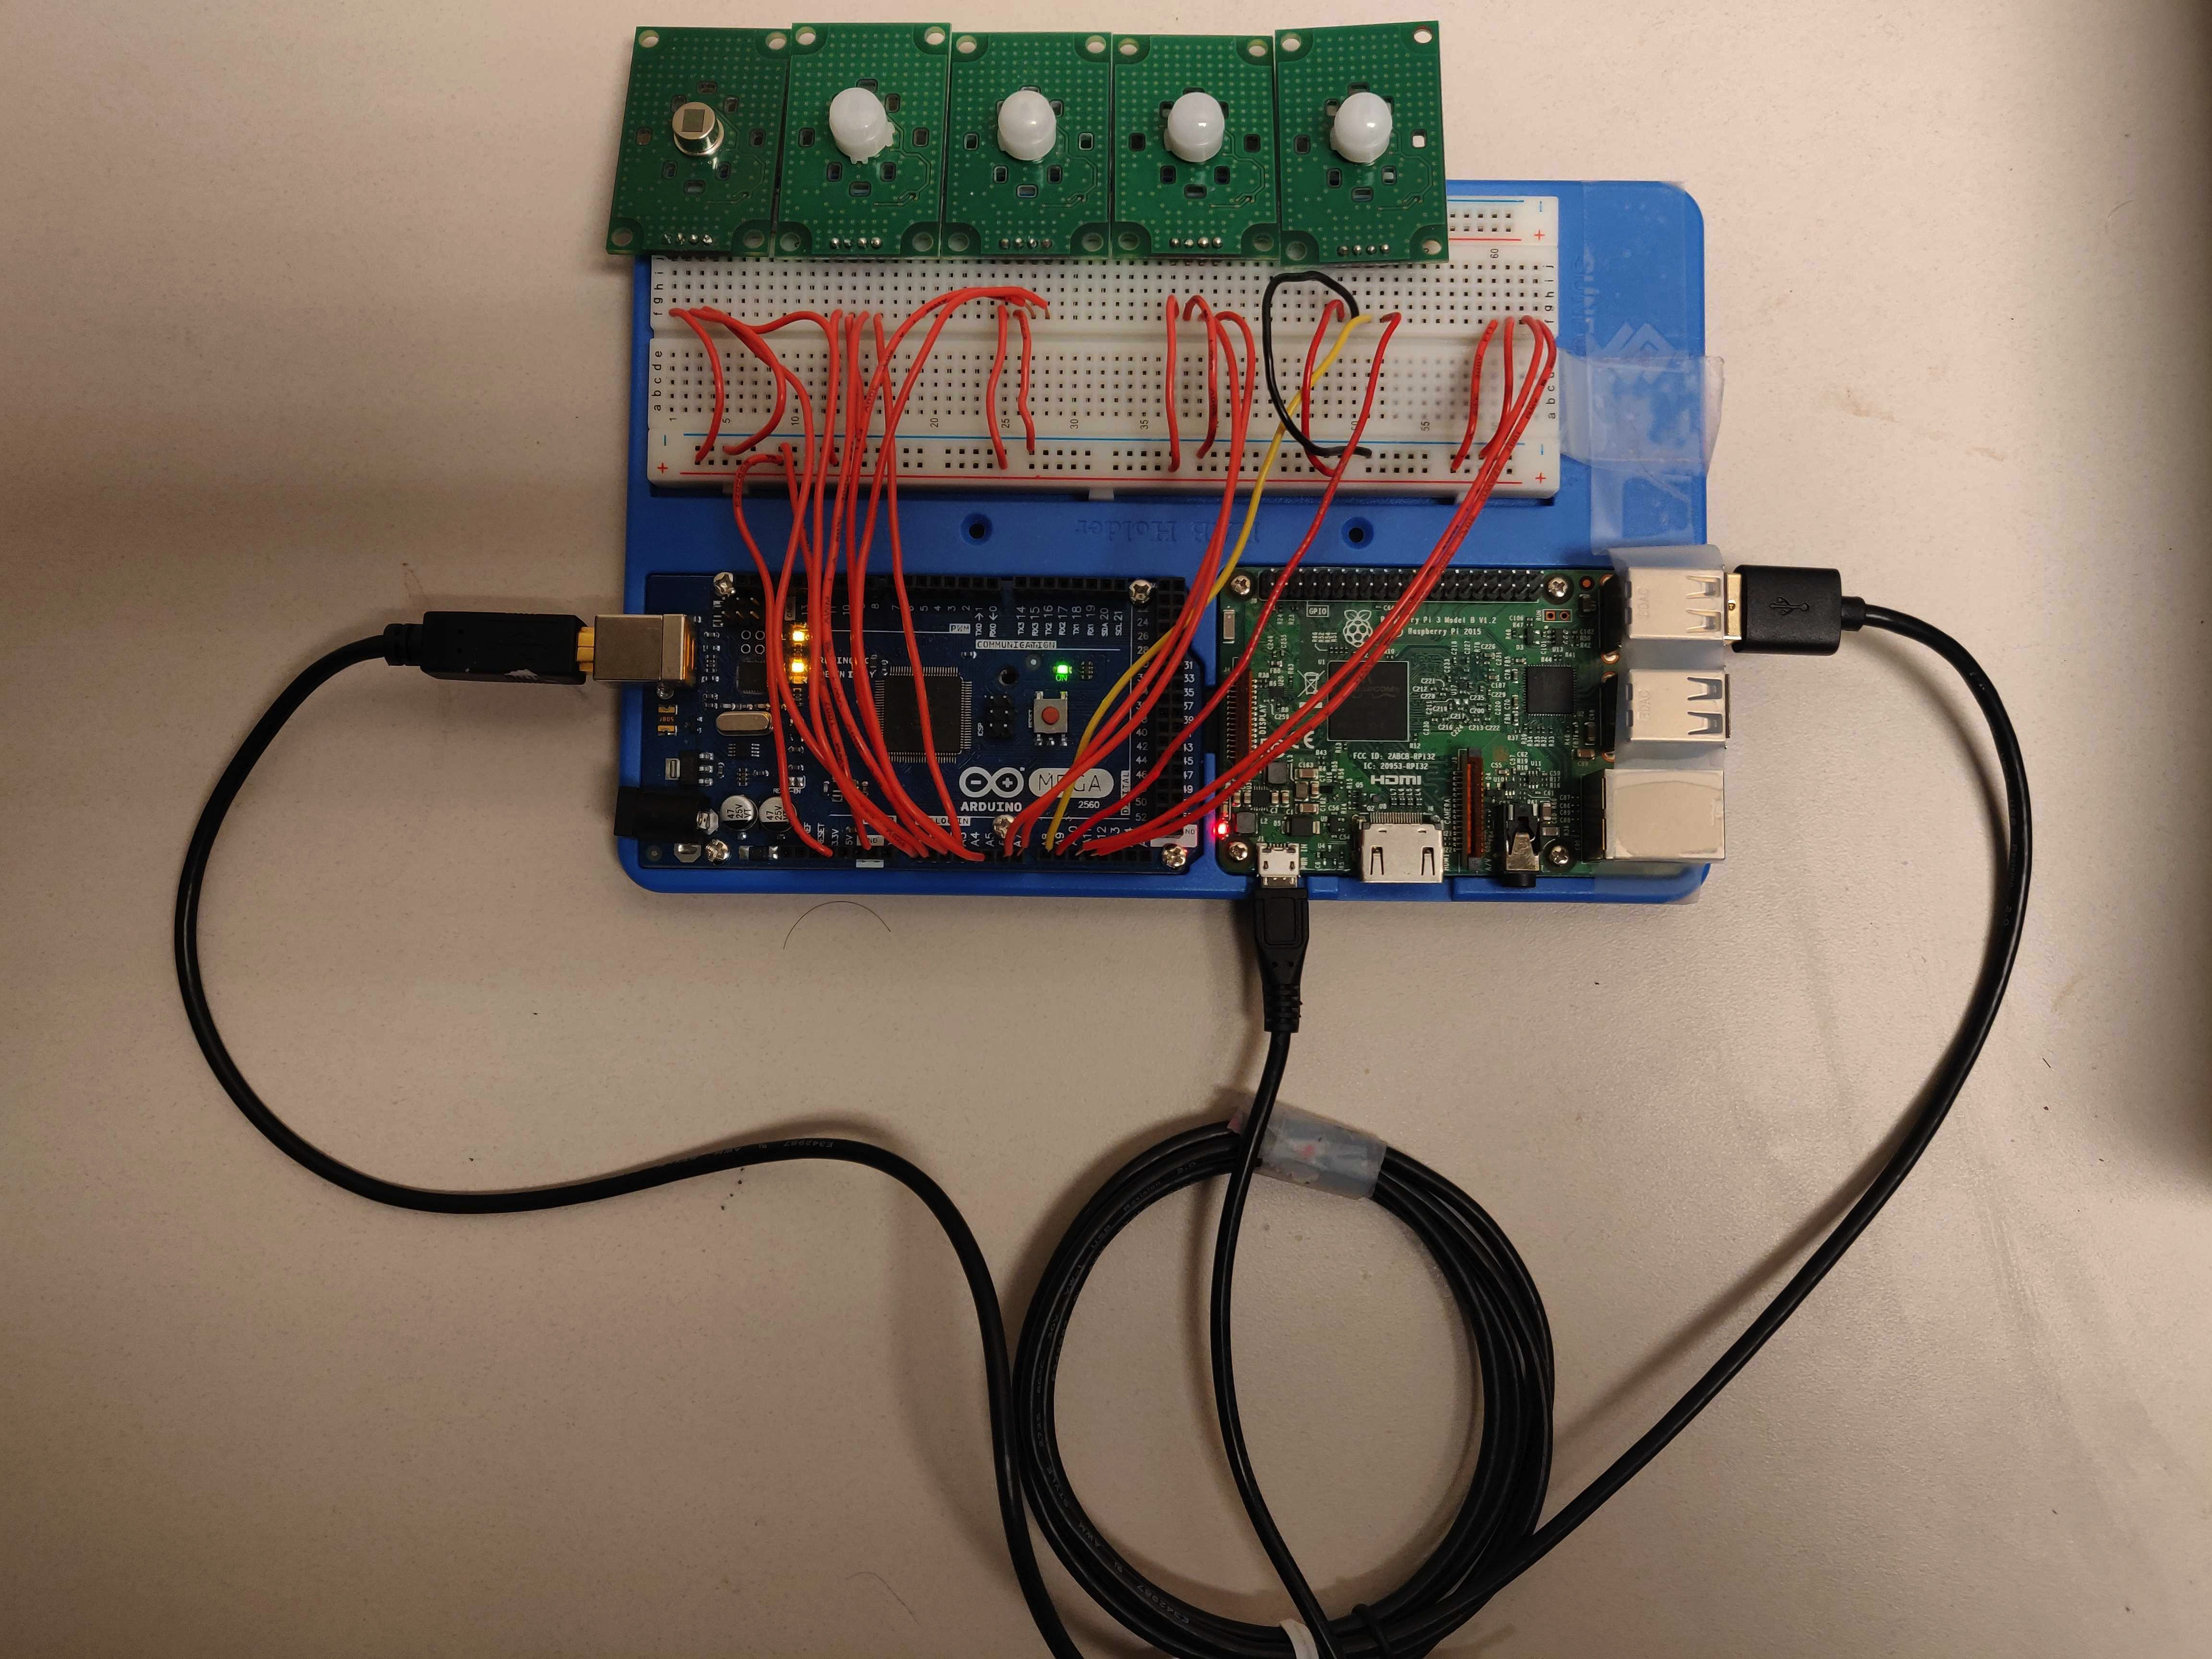
\includegraphics[scale=0.022]{figures/platform/eval_platform.jpg}
		\captionof{figure}{Evaluation Platform showing PIR sensor connected to Raspberry Pi and Arduino.}
		\label{fig:eval_platform}
	\end{minipage}
	\hfill
	\begin{minipage}[t][4cm][c]{0.70\textwidth}
		\centering
		\vspace*{\fill}
		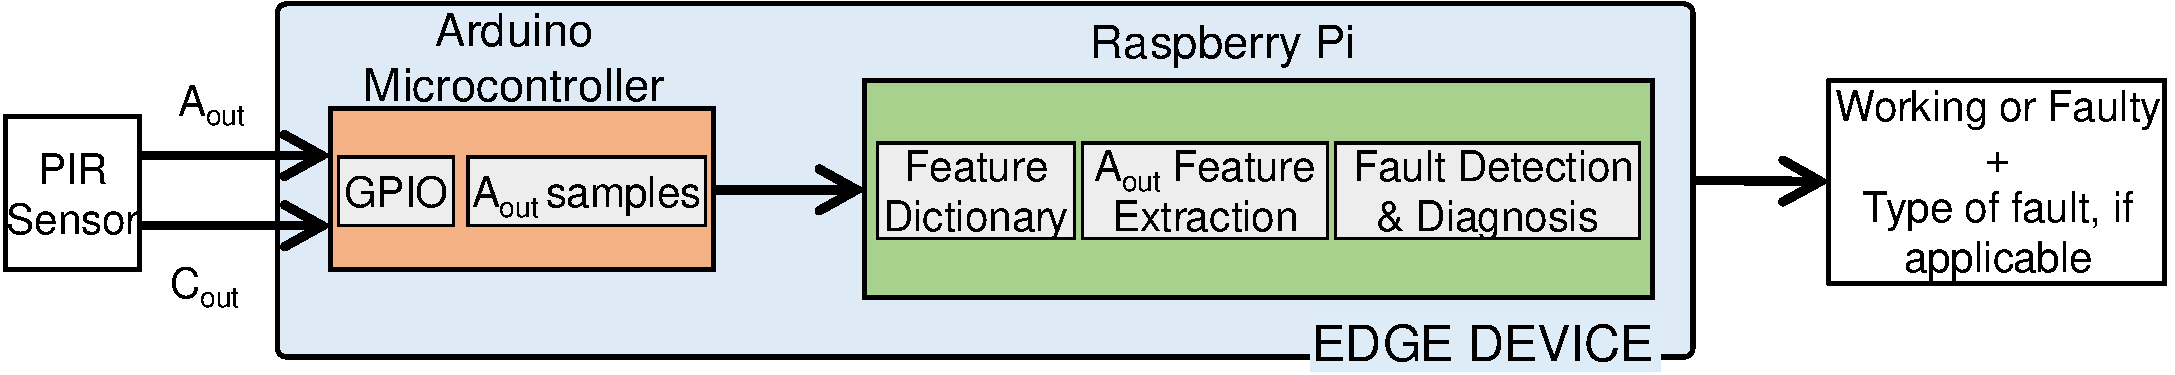
\includegraphics[width=\textwidth]{figures/platform/sensys_workflow.pdf}
		\vspace*{\fill}
		\caption{\sol workflow. The PIR sensor is connected to an Arduino microcontroller via a GPIO interface. An ADC onboard the microcontroller converts \aout and \cout values into discrete samples, that are sent to a Raspberry Pi for fault detection and diagnosis.}
		\label{fig:system_workflow}
	\end{minipage}\end{figure}

\cb \textbf{Edge Implementation} We used standard python libraries such as \texttt{tsfresh}~\cite{tsfresh2018code,christ2016distributed} for computing features such as FFT and other statistical features as a part pf feature extraction, \texttt{numpy} for data preprocessing and \texttt{xgboost}~\cite{shap_implementation} for implementing the machine learning classifiers. The end-to-end workflow of our solution is illustrated in {\bfseries Fig.~\ref{fig:system_workflow}}.

\subsection{Parameters of \sol}
\label{subsec:prac}

\ci \textbf{Size of Window}: The collected \aout waveform is split into equal-size sample windows over which features are calculated. We observed that using a window too small (\eg 128) does not allow us to capture sufficient features for a failure type and could lead to a large number of false alarms. Also, too large of a window size (\eg 8192) leads to an overlap in the features of multiple failure classes leading to a loss of accuracy. The variation of model accuracy as a function of window size is shown in {\bfseries Fig.~\ref{fig:accuracy_vs_window_size}}. We chose a window size of 1024 samples as it gave us a good trade-off between time to capture a window (approx. 50 seconds) and accuracy (> 98\%).

\begin{figure}\centering
	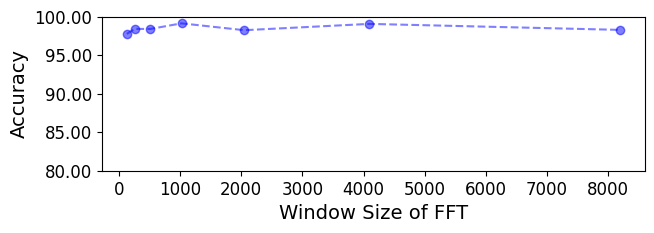
\includegraphics[width=0.48\textwidth]{figures/classification/accuracy_vs_window_size.png}
	\caption{Model Accuracy for different window sizes. We choose 1024 as the default window size.}
	\label{fig:accuracy_vs_window_size}
\end{figure}

\cii \textbf{Benjamini-Hochberg (B-H) Feature Selection} While there are more than 300 features that can be derived for time series analysis of \aout, B-H feature selection process (derived from parameterized hypothesis testing)~\cite{benjamini1995controlling,christ2018time} prunes this to a lower number of features that can sufficiently capture the physics of the system. We observed that using more than 10 features did not contribute to a significant increase in accuracy (beyond 98\%) and can, in practice, lead to lower performance due to overfitting as described in \S\ref{subsec:bh}.

\ciii \textbf{Classifier Model}: We used a Random Forest classifier~\cite{polikar2012ensemble, breiman2001random} owing to the capability to classify data based on ``entropy'' or the information gain.  Random Forest uses an ensemble of trees and has been shown to give high predictive accuracy and control over-fitting in practice, both of which are issues with decision trees. Additionally, Random Forests are amenable to interpretation by techniques such as Shapley TreeExplainer~\cite{lundberg2020local2global} that explains the features influencing prediction. \textit{Finally, we note that \aout is compatible with any classification algorithm.}

 \section{Evaluation}
\label{sec:evaluation}
The evaluation is intended to answer the following questions -- \ca can we detect failures~\ie separate faulty PIR sensors from working ones? and \cb what can we learn about the failure? In other words, can we perform diagnosis that can aid in replacing or repairing the sensor? We answer these questions in practical deployments, each consisting of the following stages:

\ca {\bfseries Stage I: Failure Detection} The goal of this stage is to isolate defective, faulty sensors from functional, working sensors. Note that we do not diagnose the failure in this stage \ie the sensors deemed faulty could be so due to multiple, as yet unknown reasons.\\
\hspace*{2ex}\cb {\bfseries Stage II: Failure Diagnosis} In this stage, we diagnose the failure by mapping it to the taxonomy defined in \S\ref{subsec:taxonomy}. Using the taxonomy as a reference, we seek to conclude whether it is the lens, pyroelectric or electronics subsystem that contains the failure.\\
\hspace*{2ex}\cc {\bfseries Stage III: Fine-Grained Fault Analysis} In this stage, we learn details about the failure as precisely as possible. \Eg if we attribute a fault to be Class III failure, we seek to narrow it down to see if it is due to deposition of dust or paper on the lens.

\subsection{Real-world Deployments}
\label{subsec:deployment}


We performed the following \emph{deployments across multiple scenarios and geographic locations,~\viz}  
\ca in the elevator of a building (\S\ref{subsubsec:elevator}), 
\cb in the lobby of a university building (\S\ref{subsubsec:lobby}), \cc in a Starbucks coffee shop (\S\ref{subsubsec:starbucks}), and \cd in a cafeteria (\S\ref{subsubsec:cafeteria}) (India).
The different deployment scenarios in \ca -- \cc are shown in {\bfseries Fig.~\ref{fig:pir_deployment_scenario}}, and aim to capture diverse environmental conditions and challenges (heat, dust, humidity~\etc).
We used 15 sensors in total across all our deployments comprising of 5 working sensors and 2 faulty sensors per class. A combination of these was used in each of our deployments. In each of these deployments, we followed the pre-deployment process, as mentioned in \S\ref{sebsec:pre_deploy}, where different types of faulty sensors were deployed for a week to collect its \aout and \cout. This pre-deployment is a one-time process to calculate different time and frequency domain characteristics capturing the physics of \aout. A subset of these sensors used in the pre-deployment was randomly picked in each of the deployments.
These sensors were deployed (\textbf{Fig.~\ref{fig:pir_sensor_failure_photographs}}) over a duration of 3 months and collected data both during times of low occupancy (weekends, late nights) and high occupancy (weekdays, working hours). Note that no auxiliary private data such as audio or video were captured during these deployments. 

\begin{figure}[t!]
	\centering
	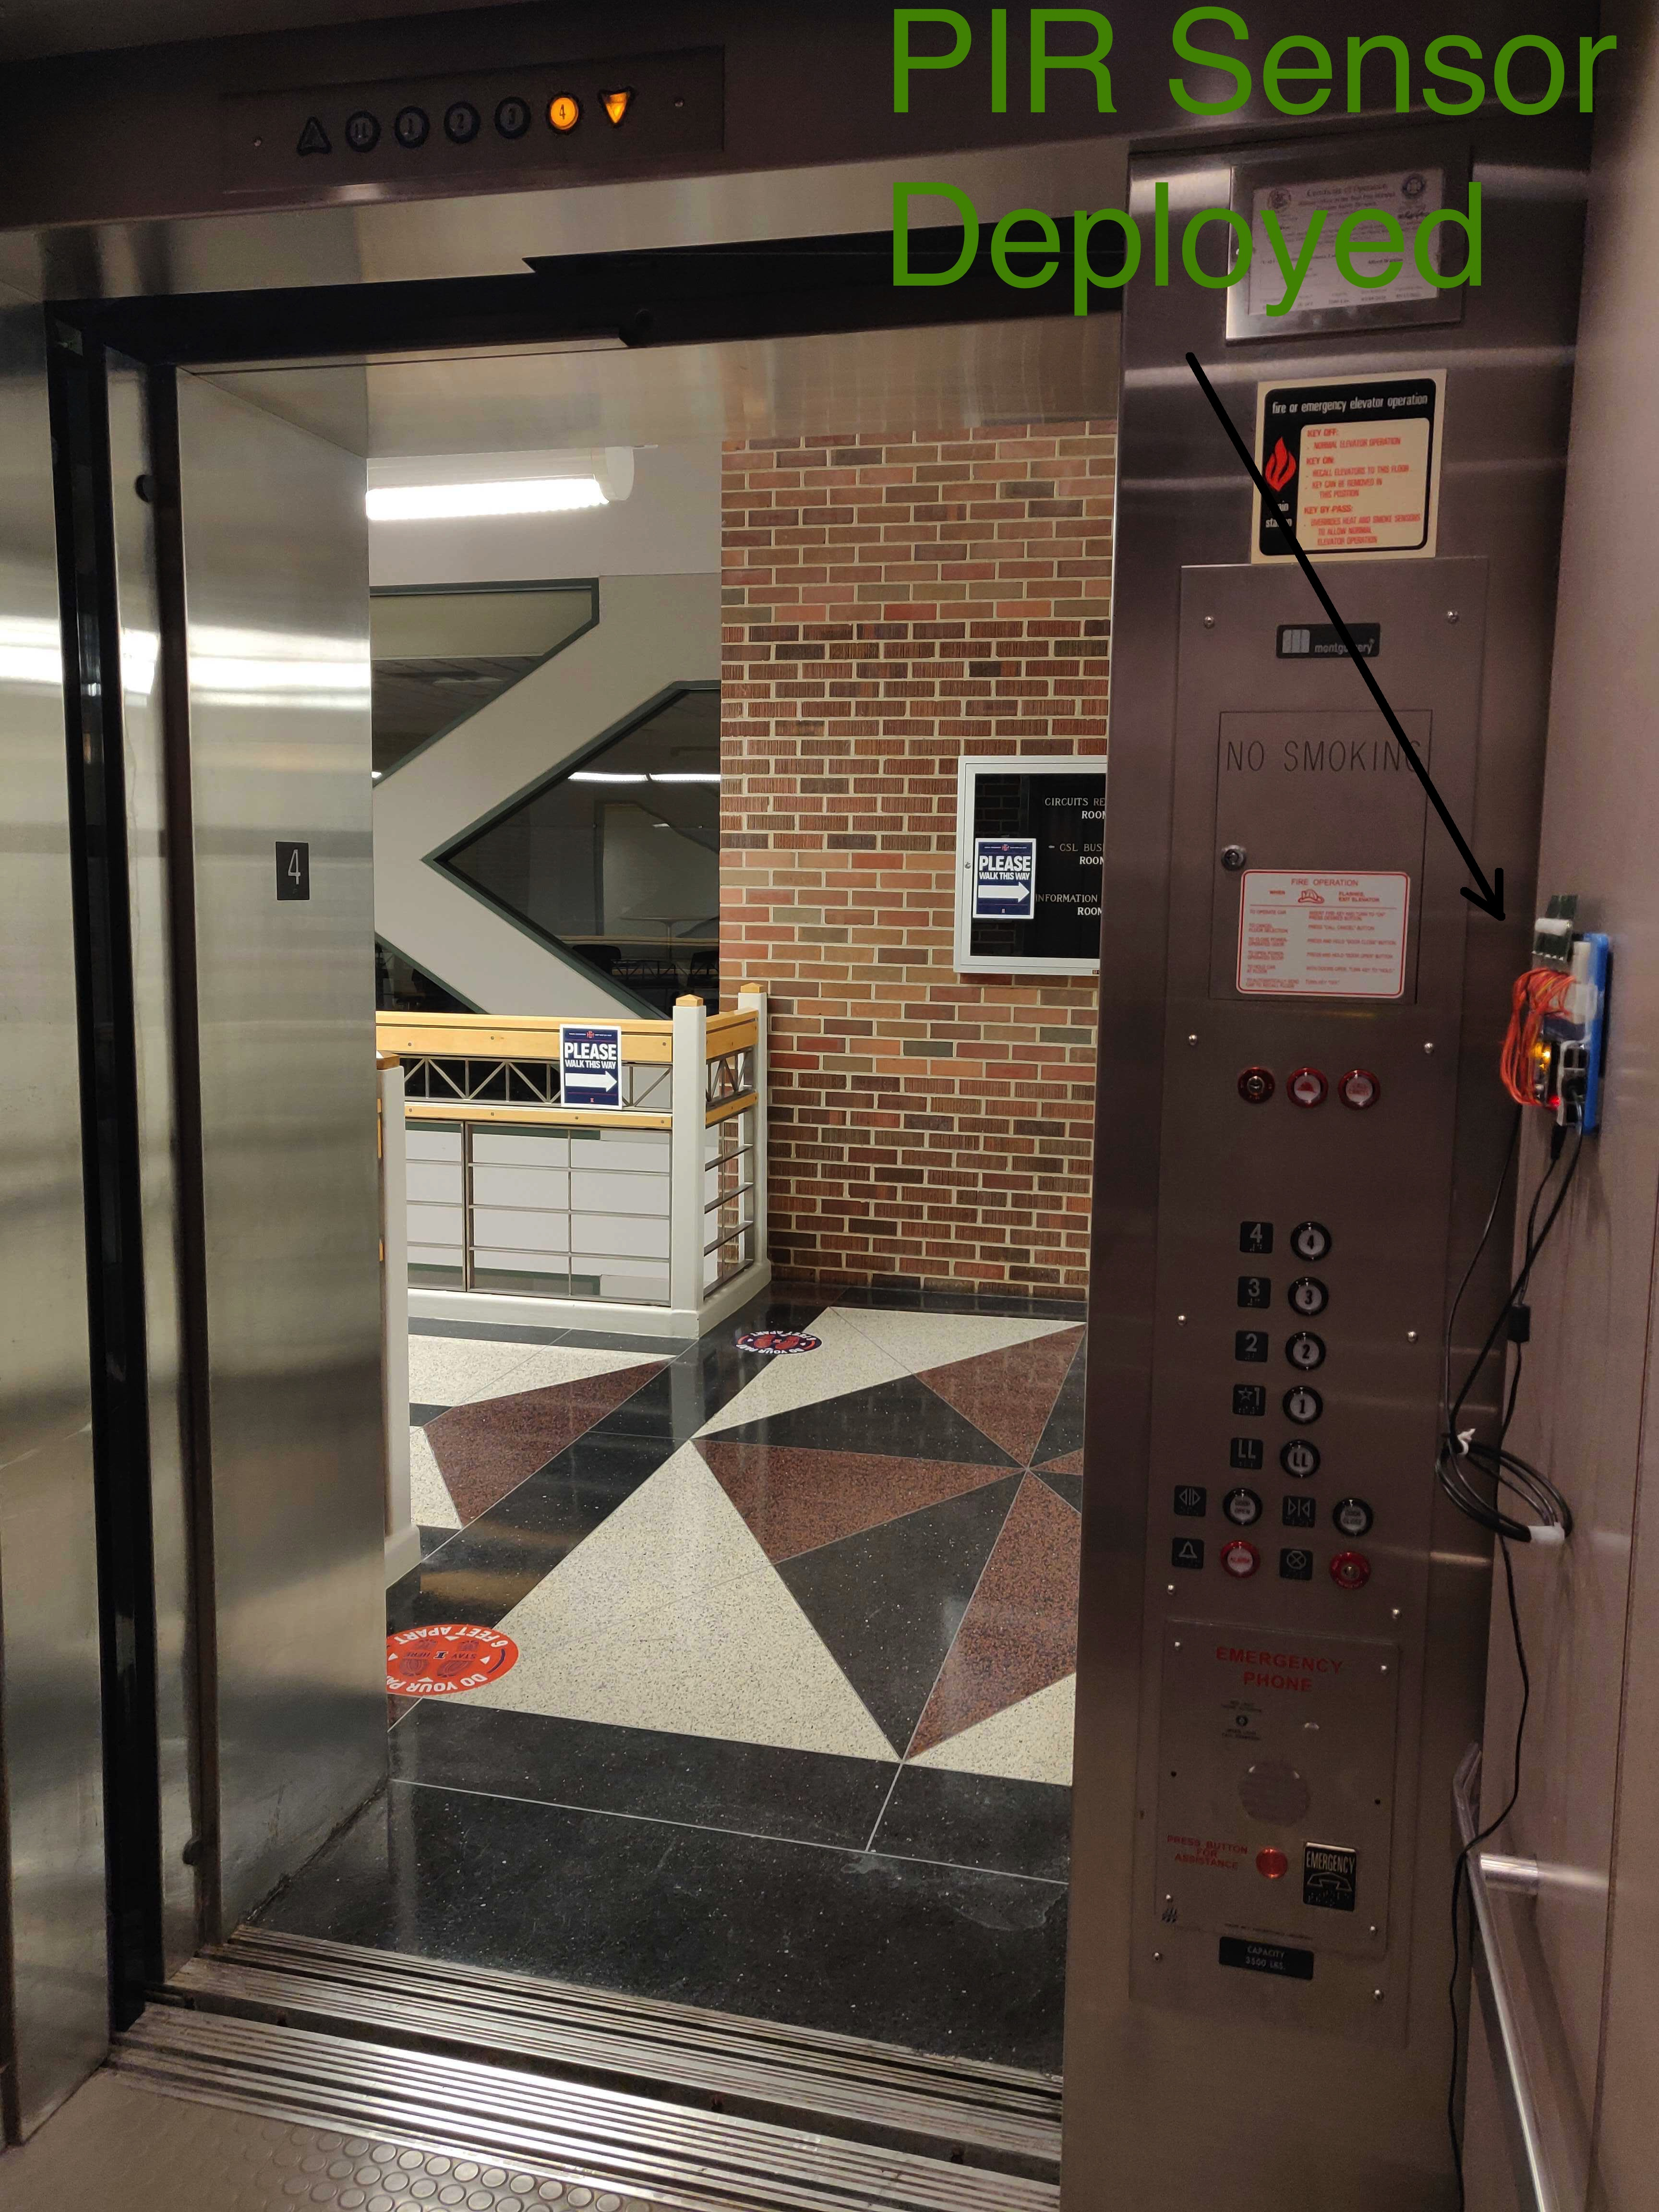
\includegraphics[width=0.3\textwidth, height=1.33in]{figures/deployment/elevator/Elevator-jpg.jpg}
	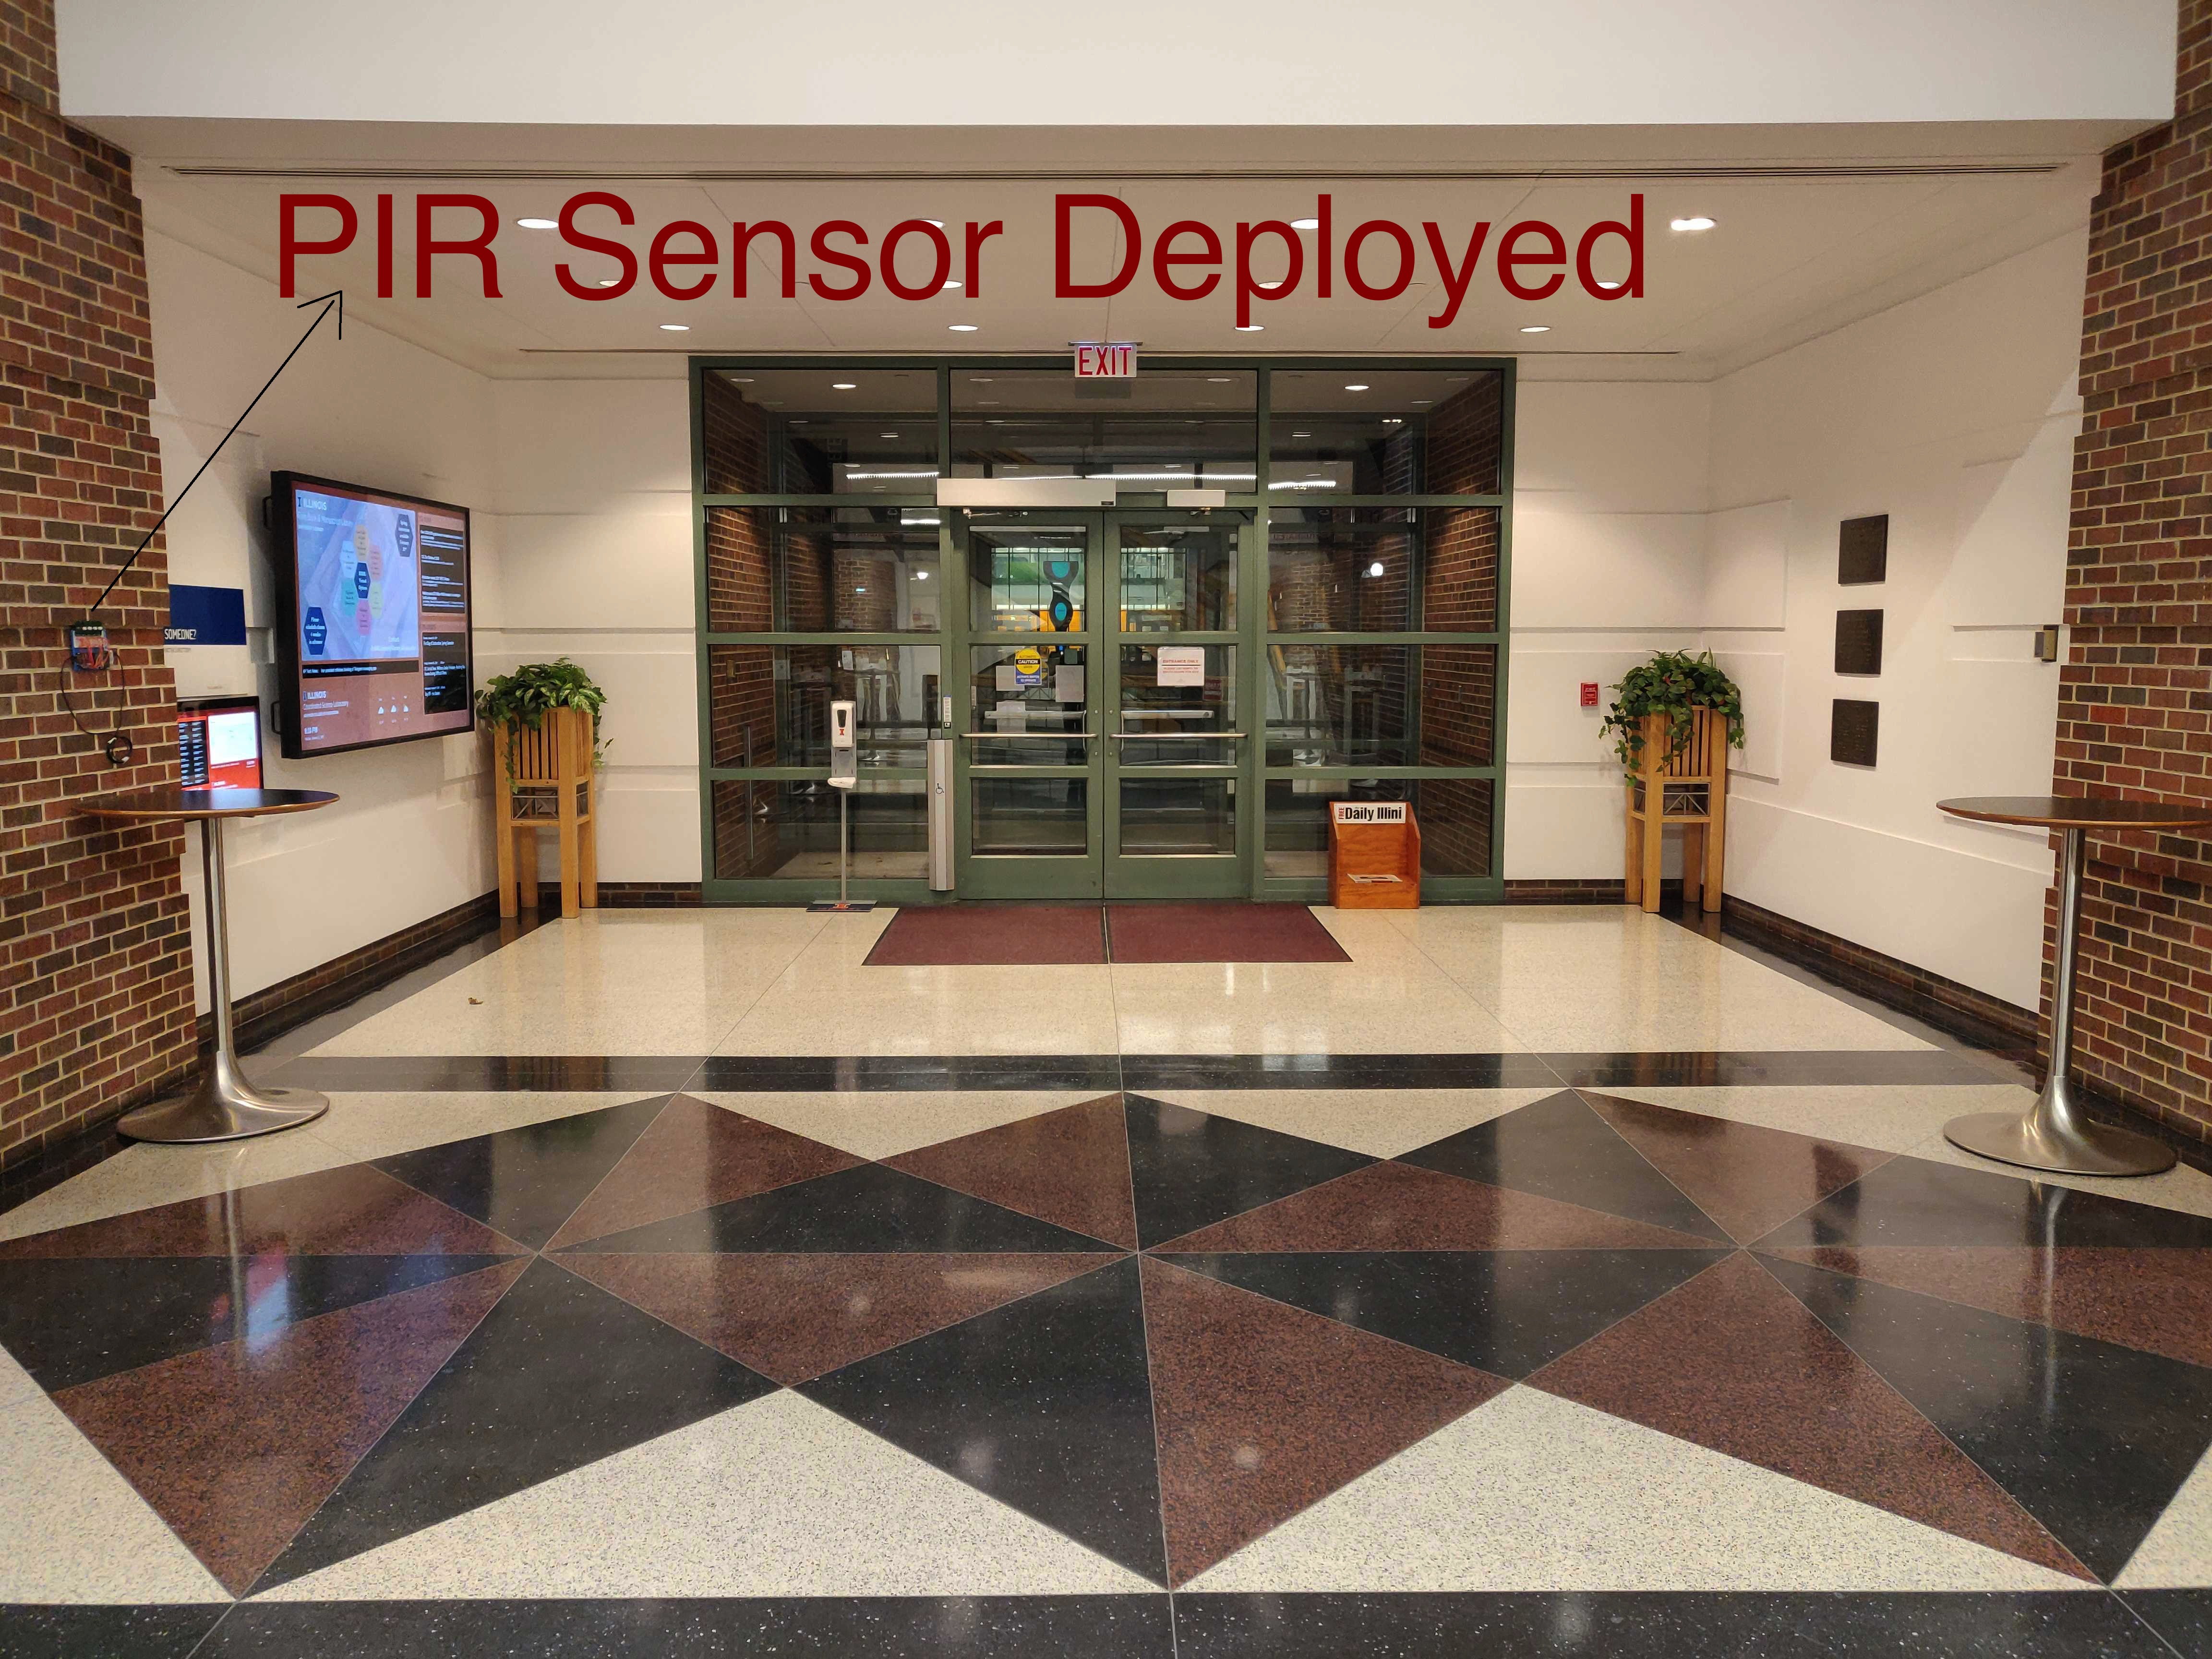
\includegraphics[width=0.3\textwidth]{figures/deployment/lobby/lobby.jpg}
	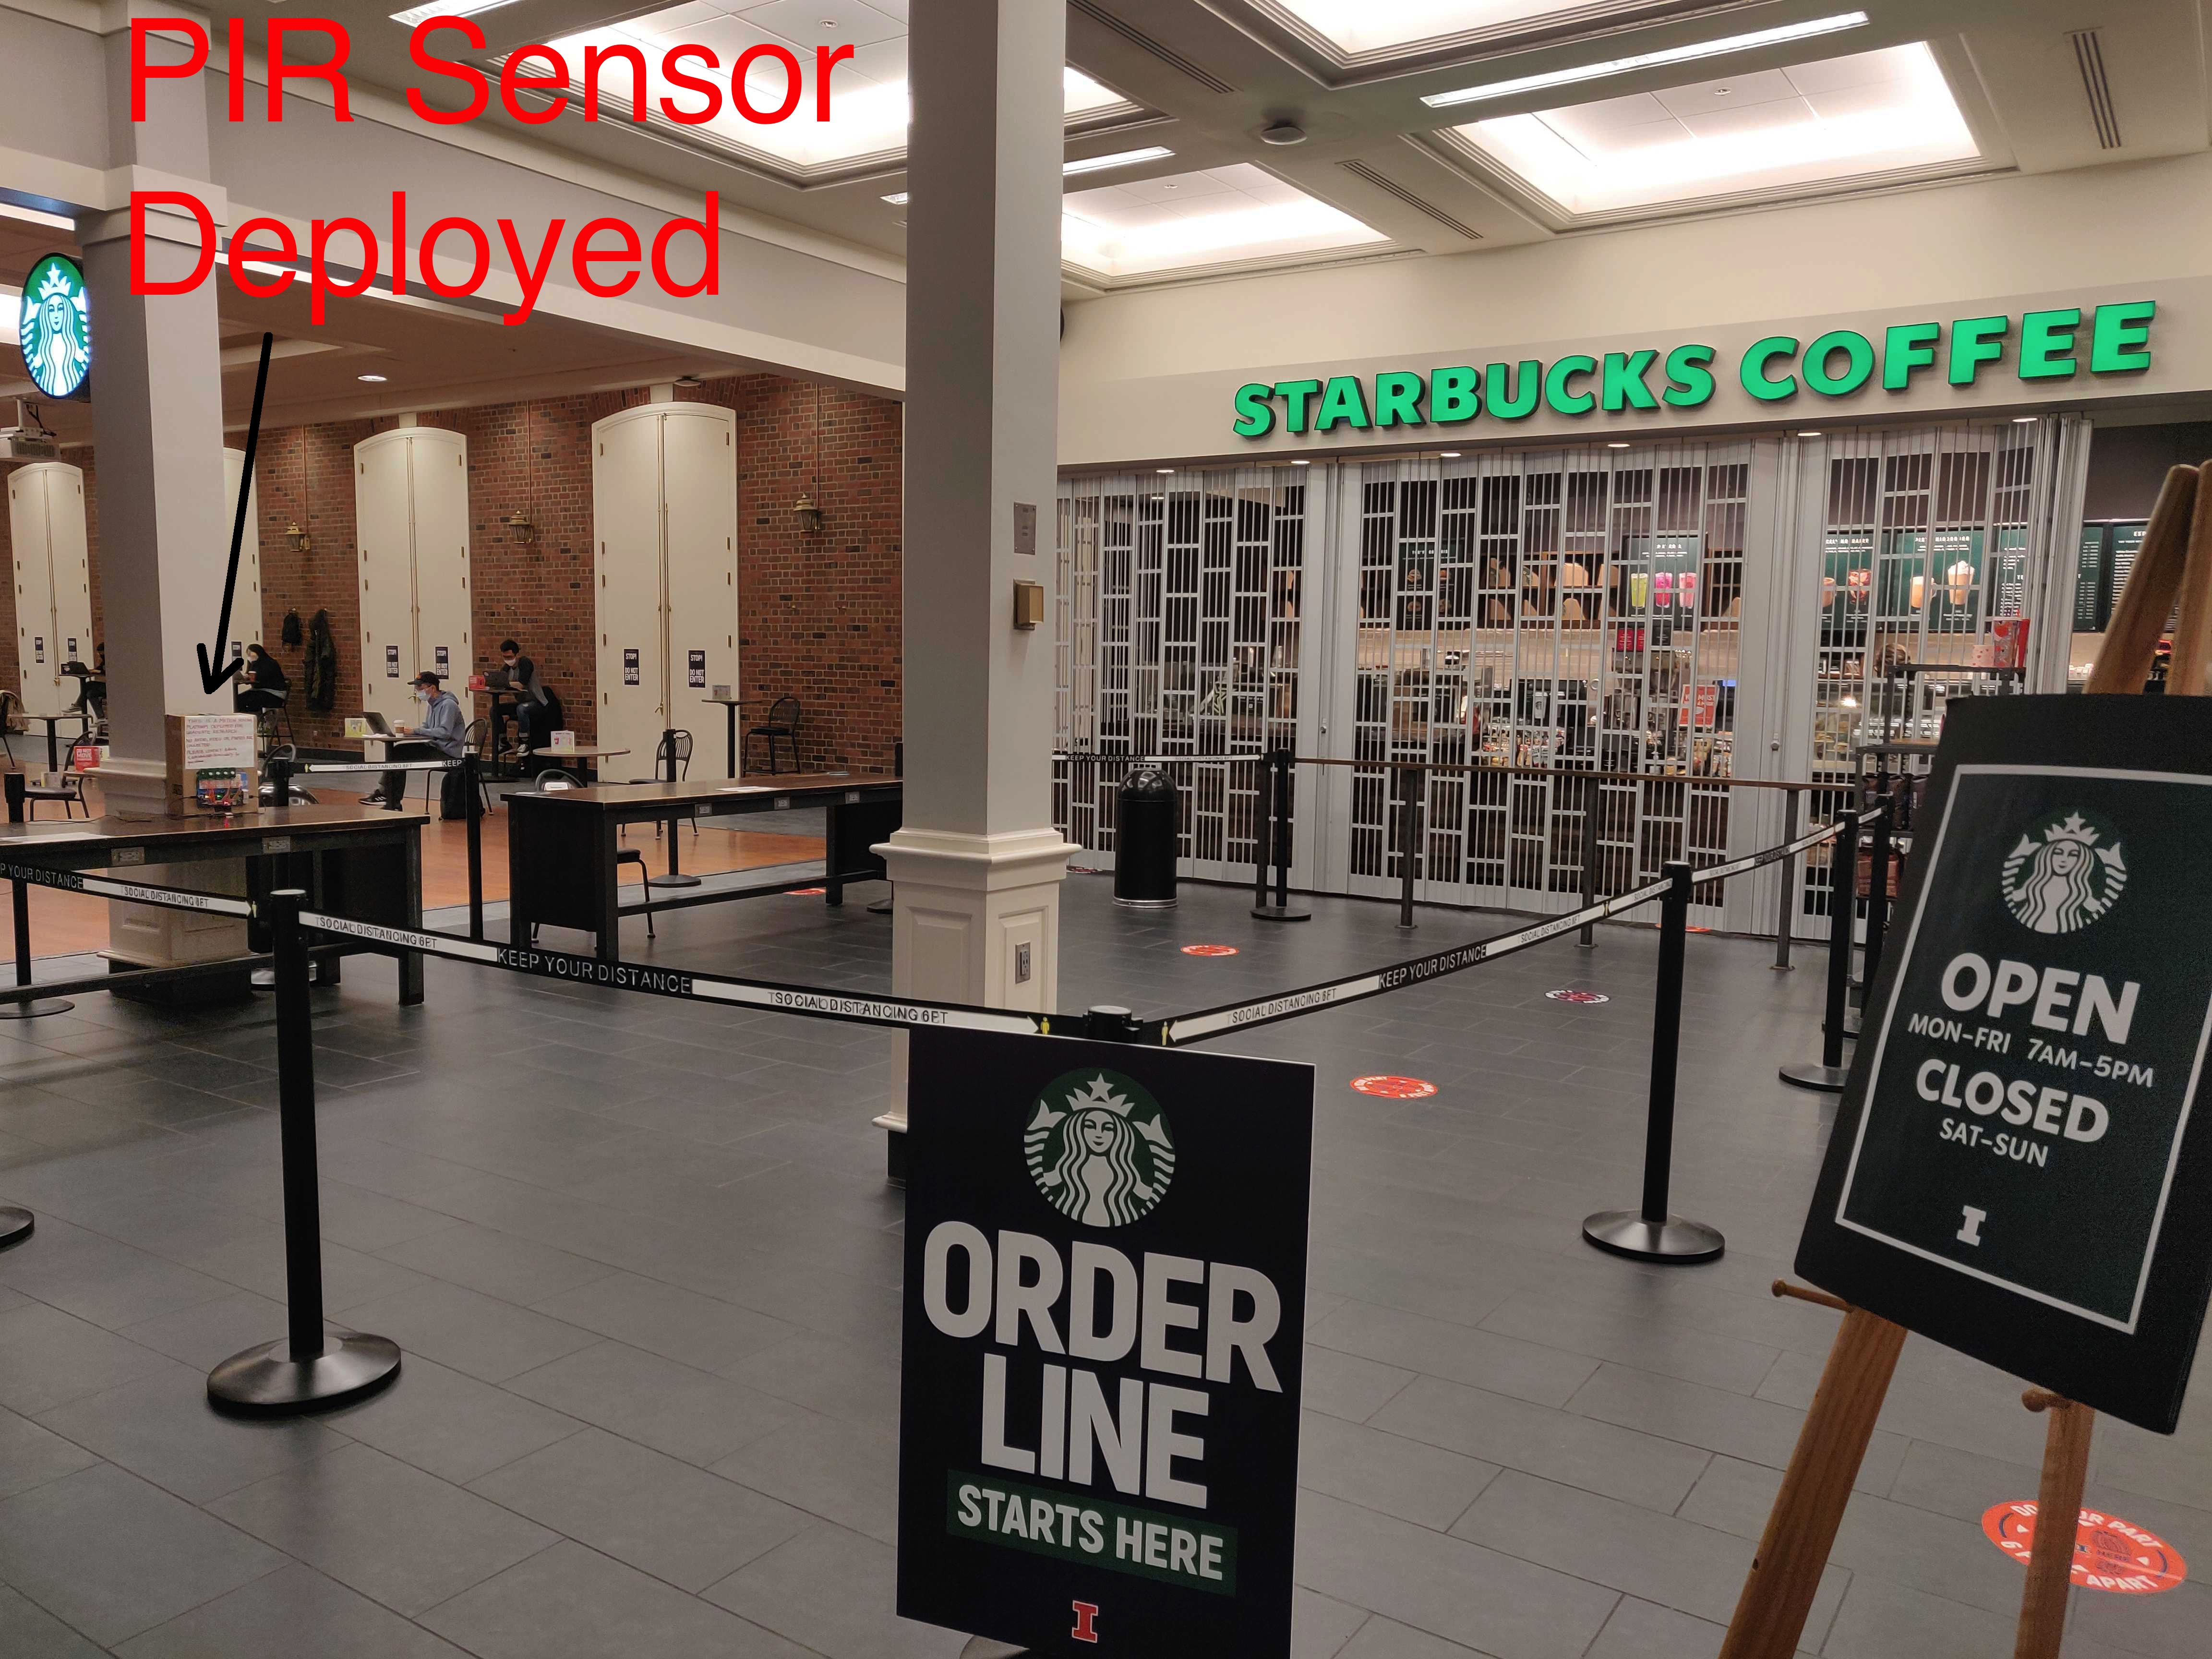
\includegraphics[width=0.3\textwidth]{figures/deployment/coffee_shop/Starbucks-jpg.jpg}
	\caption{\footnotesize{Deployment Scenarios} used for evaluating \sol in PIR sensor failure detection and diagnosis~\viz Elevator, Lobby of a building and Starbucks coffee shop.}
	\label{fig:pir_deployment_scenario}
\end{figure}
\begin{figure*}
    \begin{subfigure}[t]{0.4\textwidth}
        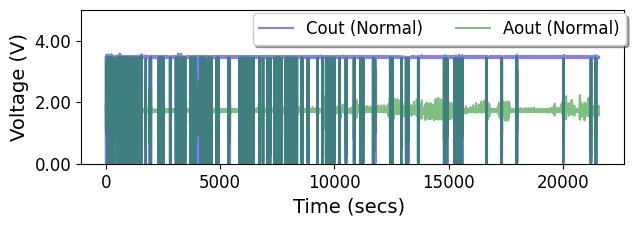
\includegraphics[width=\textwidth]{figures/deployment/elevator/afternoon-6hr.png}
    	\caption{}
    	\label{fig:deployment_csl_elevator}\end{subfigure}\hfill \begin{subfigure}[b]{0.59\textwidth}
	    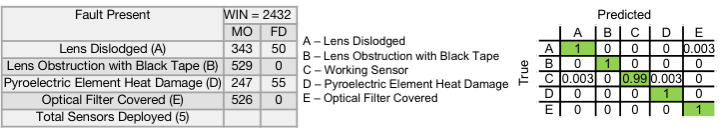
\includegraphics[width=\textwidth, height=0.65in]{figures/deployment/elevator/confusion-matrix-elevator-camera-ready.png}
		\caption{}
		\label{fig:elevator_classification_results}
	\end{subfigure}\caption{\footnotesize Elevator Deployment \ca Occupancy : The graph is a 6 hour deployment during business hours, \cb Deployment Statistics and confusion matrix of the classification model. Column titles: \textbf{WIN}$\rightarrow$Total Number of Windows, \textbf{MO}$\rightarrow$Misses Obstacle, \textbf{FD}$\rightarrow$ False Detection.}
\end{figure*}
\begin{figure*}
	\centering
	\begin{subfigure}[t]{0.4\textwidth}
		\centering
		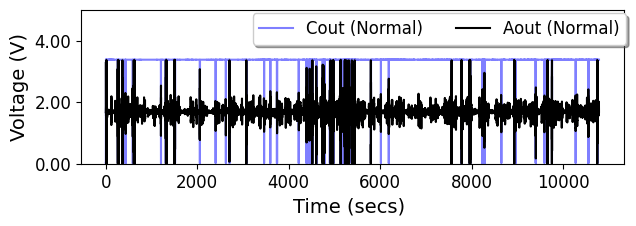
\includegraphics[width=\textwidth]{figures/deployment/lobby/lateafternoon-3hrs.png}
		\caption{}
        \label{fig:deployment_csl_lobby}\end{subfigure}\hfill \begin{subfigure}[b]{0.59\textwidth}
	    \centering
	    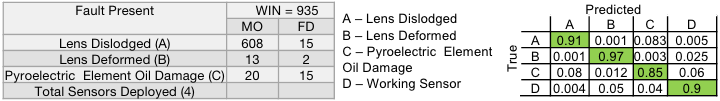
\includegraphics[width=\textwidth]{figures/deployment/lobby/confusion-matrix-lobby-camera-ready.png}

	    \caption{}
	    \label{fig:lobby_classification_results}
	\end{subfigure}
	\caption{\footnotesize Lobby Deployment \ca Occupancy graph during late evening from 6.45 pm to 9.45 pm at the lobby of our university building, \cb Deployment Statistics and confusion matrix of the classification model. Column titles: \textbf{WIN}$\rightarrow$Total Number of Windows, \textbf{MO}$\rightarrow$Misses Obstacle, \textbf{FD}$\rightarrow$ False Detection.} 
\end{figure*}
\begin{figure*}
	\begin{subfigure}[t]{0.4\textwidth}
		\centering
		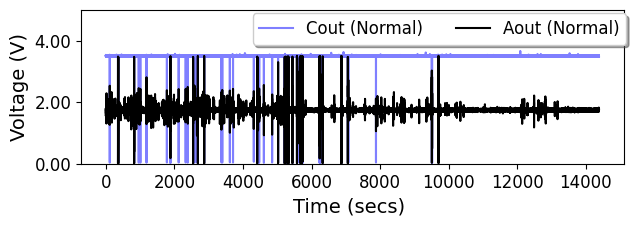
\includegraphics[width=\textwidth]{figures/deployment/coffee_shop/starbucks_4hr_deployment.png}
		\caption{}
		\label{fig:deployment_starbucks}
	\end{subfigure}\hfill \begin{subfigure}[b]{0.59\textwidth}
	    \centering
	    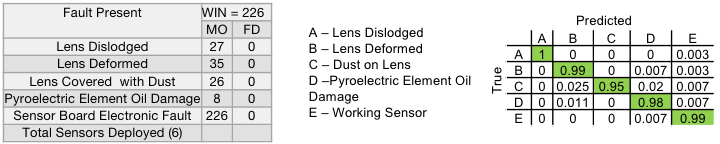
\includegraphics[width=\columnwidth]{figures/deployment/coffee_shop/confusion-matrix-coffeeshop-camera-ready.png}
	    \caption{}
	    \label{fig:coffeeshop_classification_results}
	\end{subfigure}
	\caption{\footnotesize \textbf{Starbucks Deployment Occupancy}: Evening deployment from 4.45 pm to 8.45 pm. The second half has much lesser little foot traffic. \cb Deployment Statistics and confusion matrix of the classification model. Column titles: \textbf{WIN}$\rightarrow$Total Number of Windows, \textbf{MO}$\rightarrow$Misses Obstacle, \textbf{FD}$\rightarrow$ False Detection. }
\end{figure*}


\subsubsection{Deployment in a University Elevator (US)}\label{subsubsec:elevator} 
We deployed working and faulty sensors along the inside wall of an elevator in our university research building (left {\bfseries Fig.~\ref{fig:pir_deployment_scenario}}). The data collection captured scenarios of both high and low occupancy during and outside of business hours. In addition to faulty sensors, we placed a normal, working sensor to keep track of the actual motion in the elevator. 
{\bfseries Fig.~\ref{fig:deployment_csl_elevator}} plots \cout and \aout values captured by the working sensor showing the actual traffic in the elevator on one of the days.Vertical stripes on the graph showing oscillations of \cout (in blue) are points of occupancy \ie denoting a person's entry/exit at the elevator. Likewise, regions of graph with no occupancy is represented by a flat line, hovering around 3.7 V. 

\newcommand{\elevatortable}{\footnotesize
		\centering
		\begin{tabular}{ | l | c | c | }
			\hline
			\multirow{2}{*}{\bfseries \textsc{Fault Present}} & 
			\multicolumn{2}{c|}{\bfseries WIN = 2432} \\
			\cline{2-3}
			& \bfseries MO &  \bfseries FD \\ \hline \hline
			Lens Dislodged &  343 & 50   \\ \hline
			Lens Covered with Black Tape &  529 & 0   \\ \hline
			Pyroelectric Element Heat Damage &  247 &  55 \\ \hline
			Optical Filter Covered & 526 & 0  \\ \hline
			Sensor Board Short & 529 & 0 \\ \hline
		\end{tabular}			
}




For faulty sensors, we measure the number of time windows where an obstacle was captured or missed. 
The performance of faulty sensors relative to a working sensor is tabulated in {\bfseries Fig.~\ref{fig:deployment_csl_elevator}}. 
When the lens cap is dislodged, it misses obstacles in 343 time windows whereas the (thermal) breakage of the pyroelectric element results in 247 misses. 
Overall, we observe that missed obstacles are more common than false alarms.
This ties into common observations in conference rooms operated with PIR sensor-controlled lighting, where lights turn off even with occupants present.


As described in \S\ref{subsec:high_level_algorithm}, \sol collects the \aout signals and uses a machine learning model on their extracted features detect faulty sensors. Using a random forest classifier, we obtain the confusion matrix ({\bfseries Fig.~\ref{fig:elevator_classification_results}}), which shows that predicted label matches the true label for each failure. 
We note that -- \ca the working sensor has distinct characteristics compared to the faulty sensors and is isolated correctly, \cb faulty sensors with different failures in lens and pyroelectric subsystem are identified to the failure class correctly as observed by diagonal of the confusion matrix. This implies that the features of \aout, derived by \sol is able to differentiate between lens being dislodged, lens being covered with tape, oil condensation on the optical filter and heat damage on the pyroelectric element.



\subsubsection{Deployment in a University Lobby (US)}\label{subsubsec:lobby} We deployed our sensors in the first floor lobby space of our university building (center {\bfseries Fig.~\ref{fig:pir_deployment_scenario}}). The lobby deployment is noisier with fewer constraints on direction of motion, compared to the confined space of an elevator. As in the elevator deployment, we deployed a combination of working and faulty sensors shown in the table in {\bfseries Fig.~\ref{fig:lobby_classification_results}}.


\textbf{Fig.~\ref{fig:deployment_csl_lobby}} shows a 3 hour slice of the deployment. The vertical stripes on \cout correspond to traffic entering/exiting the lobby in the field of view. 
The performance of the sensors deployed, in terms of false detection and missed obstacles, is shown in the table in {\bfseries Fig.~\ref{fig:lobby_classification_results}}. The sensors with lens dislodged missed a large amount of obstacles. This is due to the lack of focus of thermal radiation on the pyroelectric element resulting in dispersion of radiation due to the large lobby area. As a result of this failure, only obstacles that line up in the reduced field of view, are captured. This issue is not present in an elevator due to its confined space.
Other faults such as lens deformation and damage due to oil condensation experienced lesser number of misclassifications. 
Upon extracting the features of the \aout signals, and classifying it using the procedure in \S\ref{subsec:high_level_algorithm}, we observe the confusion matrix as shown in {\bfseries Fig.~\ref{fig:lobby_classification_results}}. The high fraction along the diagonal shows that a majority of sensor failures are classified and identified correctly, as the features are able to bring out differences in the physics of failures.
Note that we observe some misclassifications of sensor faults (\eg for C). We argue that this is due to the deployment area of a lobby being open and the limited coverage area of the sensor, both of which can lead to imperfect capture at the periphery. Consequently, for traffic at the edges of field of view, this reduced thermal radiations could lead to some misclassifications. 

\begin{figure*}
	\begin{minipage}[t]{0.48\textwidth}
		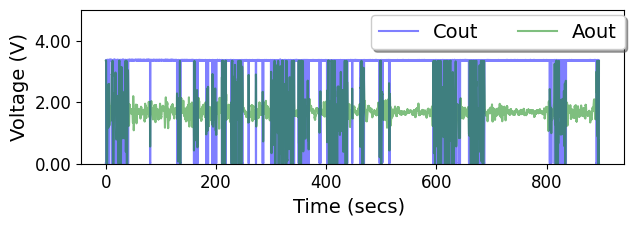
\includegraphics[width=6cm]{figures/deployment/bangalore-cafetria/msr-cafeteria-15mins.png}
		\vspace{-5pt}
		\caption{\textbf{Cafeteria Deployment occupancy} during lunchtime. A 15 min. slice of traffic at the checking counter.}
		\label{fig:deployment_msr_cafeteria}
	\end{minipage}
	\hfill
	\begin{minipage}{0.48\textwidth}
		\vspace{-\baselineskip}
		\begin{tabular}{l c c c c c}
			\hline
			\textbf{Training (MB)} & \textbf{32} & \textbf{64} & \textbf{96} & \textbf{112} & \textbf{128} \\
			\hline \hline
			Accuracy (\%) & 92.4 & 95.8 & 98.6 & 99.1 & 99.4 \\
			\hline
		\end{tabular}
		\vspace{\baselineskip}
		\caption{\textbf{Failure detection accuracy} as a function of the size of training dataset}
		\label{fig:dataset_size}
	\end{minipage}
\end{figure*}

\subsubsection{Deployment in a Starbucks (US)}\label{subsubsec:starbucks}
We deployed PIR sensors near the ordering queue of the coffee shop during business hours to capture the typical foot traffic (right {\bfseries Fig.~\ref{fig:pir_deployment_scenario}}).
Our deployment captured linear, regularized bidirectional movement (entry followed by exit of the region of interest) ({\bfseries Fig.~\ref{fig:deployment_starbucks}}).
Our deployment lasted for a duration of 4 hours on a busy Friday evening.
We observed that out of 226 time windows (each containing 1024 samples), there were missed obstacles across: \ci 27 windows in class I, \cii 35 windows in class II, \ciii 26 windows in class III and no windows in class IV. The missed obstacles and false detection (none in this case) are summarized in {\bfseries Fig.~\ref{fig:coffeeshop_classification_results}}.
Using \sol, we observe high fractions along the diagonal of the confusion matrix; hence the predicted label of sensor failure matches the true label.

Furthermore, despite the oil impurity not being enough cause it to alter performance, we still classify it is a separate class from the physics point of view due to its different behavior of \aout from that of a working sensor.
Thus, in line with the previous deployments, we can use the features of \aout to form a signature of the physics. 

\begin{figure}\centering
	\begin{subfigure}[t]{0.33\linewidth}
		\centering
		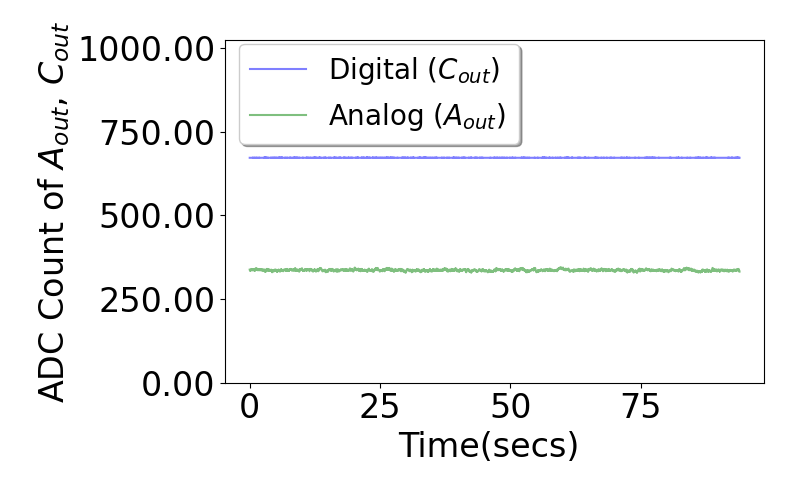
\includegraphics[width=\textwidth]{figures/pir/lens_fault/BuildSys_Graphs/CapCovered_NoObstacle.png}
		\caption{Lens Covered Completely}
		\label{fig:capcovered}
	\end{subfigure}
	\begin{subfigure}[t]{0.33\linewidth}
		\centering
		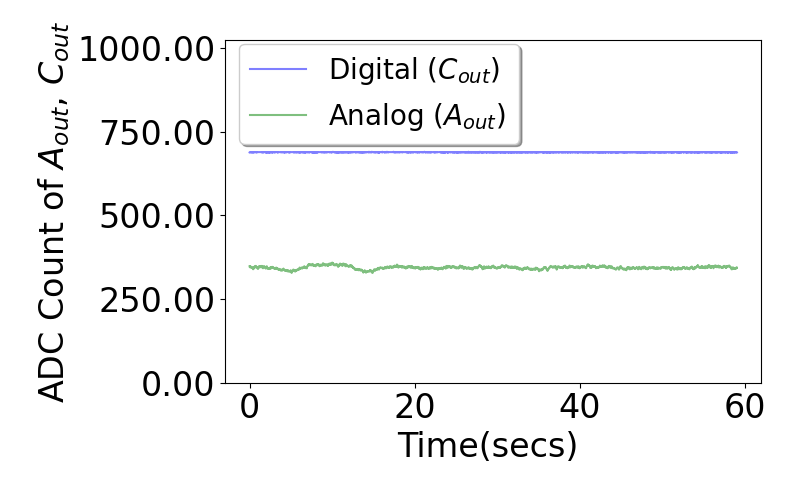
\includegraphics[width=\textwidth]{figures/pir/lens_fault/BuildSys_Graphs/CapON_NoObstacle.png}
		\caption{Lens in Place (Working)}
		\label{fig:capon}
	\end{subfigure}
	\begin{subfigure}[t]{0.33\linewidth}
		\centering
		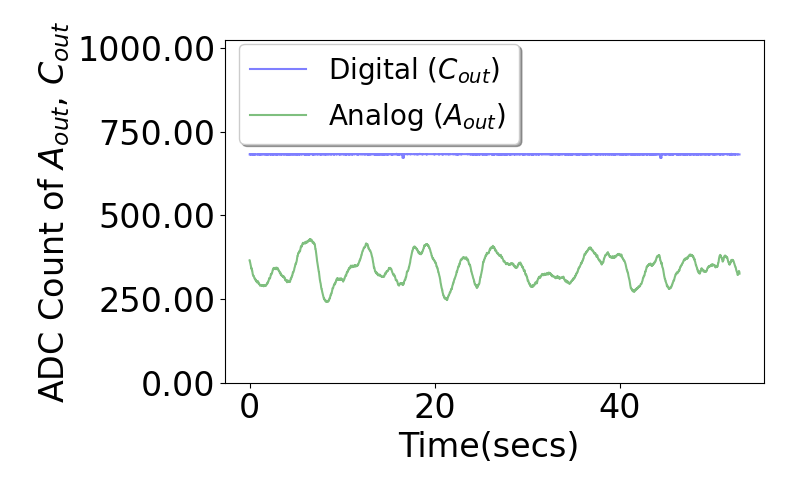
\includegraphics[width=\linewidth]{figures/pir/lens_fault/BuildSys_Graphs/CapOff_NoObstacle.png}
		\caption{Lens Dislodged}
		\label{fig:capoff}
	\end{subfigure}
	\caption{The variance in \aout during known quiet times contains hints about lens failures in the PIR sensor.}
	\label{fig:variance_cap_cases}
\end{figure}

\subsubsection{Deployment in a Cafeteria}\label{subsubsec:cafeteria} To evaluate the analysis of \aout during quiet times, we deployed a mix of 3 types of sensors with lens failures -- lens fallen off, lens covered and some working sensors during the lunch hour at a cafeteria in India. The traffic during lunchtime in the cafeteria is as shown in {\bfseries Fig.~\ref{fig:deployment_msr_cafeteria}}. As these were lens-related failures, we looked at the time-domain characterization of \aout during quiet times to understand the status of lens. The time domain representation of \aout, during a period of no occupancy, is as shown in {\bfseries Fig.~\ref{fig:variance_cap_cases}}. The y-axis is plotted in terms of the 10-bit ADC representations of voltage to highlight the differences. For a 10-bit ADC, 1023 units (\ie $2^{10} - 1$) corresponds to a voltage of 5 V. Therefore, a voltage of 1.8 V corresponds to 340 units.

We note visually that the noise floor at output of the lens subsystem is higher with the lens dislodged ({\bfseries Fig.~\ref{fig:capoff}}) as compared to both a normal sensor ({\bfseries Fig.~\ref{fig:capon}}) and one with lens covered ({\bfseries Fig.~\ref{fig:capcovered}}). Specifically, we observed a variance of 10 $Volt^2$ when lens was covered, 250 $Volt^2$ when lens was in place and working, and 1500 $Volt^2$ when lens had fallen of completely. Consequently, a low threshold ($T_L$) of 100 $Volt^2$ and a high threshold ($T_H$) of 1000 $Volt^2$ was sufficient to separate between the 3 types of sensors. Note that the variance had to be computed during a quiet period of no traffic in this case. 

We now discuss the different stages of \sol, as enumerated in the beginning of this section. 

\subsection{Stage I -- Failure Detection}
\label{subsec:fail_detection}

We aggregated all the sensors (both working and faulty) to \textit{separate faulty sensors (without specifying which class) from working sensors}. 
We collected FFT coefficients of \aout on a pre-deployment lasting 1 week and performed daily collection of \aout signals from all the deployed sensors. 
We used a Random Forest classifier with specifications shown in {\bfseries Fig~\ref{fault_detection_results}}. 
Once predicted, we manually verified the true status of the sensor and observed an accuracy of over 99\% in predicting if the sensor is working or faulty. 
Thus, FFT-based features of \aout were able to capture the physics, and hence separate faulty sensor physics from working sensor physics.
We also varied the \textit{size of training dataset} (128 MB corresponds to 1 week pre-deployment) to show the robustness of failure detection in {\bfseries Fig.~\ref{fig:dataset_size}}.


\begin{wrapfigure}{lr}{0.5\textwidth}
	\centering
	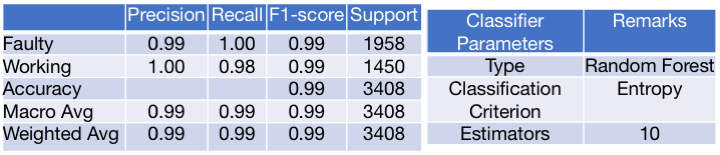
\includegraphics[width=0.5\textwidth]{figures/classification/FaultDetectionResults.png}
	\caption{\footnotesize Fault Detection showing that faulty sensors isolated from working sensors by extracting FFT of \aout and using a Random Forest Classifier.}
	\label{fault_detection_results}
\end{wrapfigure} \subsection{Stage II -- Failure Diagnosis}

Diagnosing the \textit{cause of failures (\ie class)} requires further investigation of \aout from faulty sensors.
We combine our understanding of the PIR sensor \ie physics from \S\ref{subsec:physics}, failure taxonomy from \S\ref{subsec:taxonomy} and the frequency analysis of failures from \S\ref{subsec:freq_char} and feature analysis from \S\ref{subsec:bh} -- \S\ref{subsec:shap}.
{\bfseries Fig.~\ref{fig:cdf_combined_all}} plots the CDF of FFT coefficients obtained for working sensors and various faulty sensors.
The figure shows that although the distribution of working sensors (bottom-most curve) is distinct from failed sensors, different classes of failures have distributions that are not easily separable.
Thus, relying on merely the FFT is insufficient.
Consequently, we look at an additional 10 features as described in \S\ref{subsec:bh} --- \S\ref{subsec:shap} and shown in {\bfseries Fig.~\ref{fig:BH_feature_selection}}.


We validated this across the multiple deployments in the wild --- Elevator (\S\ref{subsubsec:elevator}), Lobby (\S\ref{subsubsec:lobby}), Starbucks (\S\ref{subsubsec:starbucks}) and Cafeteria (\S\ref{subsubsec:cafeteria}).
Our real-world measurements demonstrate that features of \aout extracted during training and B-H feature selection is robust to variations in shapes and sizes of obstacles.

\subsection{Stage III -- Fine-Grained Failure Analysis} In fine-grained fault analysis, we point to the \textit{precise reason} for the fault where applicable. For example, in Class III faults it is useful to distinguish between different foreign substances contaminating the lens that can cause poor performance.


To investigate this, we selected the set of faulty sensors identified as Class III faults in Stage II: some covered with paper, some with plastic tape and some with dust and observe the \aout output closely. Although all the failure scenarios result in the obstacle being missed, frequencies present in \aout are different in each case, as shown in {\bfseries Fig.~\ref{fig:finegrained_aout}}, due to the distinct thermal absorption characteristics of the materials.
Hence, we observe that the \aout features can separate Class III failures into different fine-grained sub-classes as shown in {\bfseries Fig.~\ref{fig:finegrained_classification_results}}.

It is to be noted that fine-grained fault analysis does not work in all cases.
For example, differentiating between a lens puncture (a hole in the lens) and a lens deformation (defect in lens curvature), both examples of Class II failures, is complex. This is because both lens puncture and lens deformations lead to blind spots in the frequency spectrum. Thus, we need to use knowledge of the subsystem physics before applying the fine-grained analysis.

\noindent {\bfseries Summary:} \ci The FFT representation of \aout is used to perform binary classification between working and faulty sensors, \cii Considering multiple direct and derived time and frequency domain signal characteristics of \aout can diagnose the cause of failure in the sensor and \ciii Fine-grained fault analysis is possible in select failure cases (\eg Class III) by reanalyzing the \aout waveforms.

\begin{figure*}\begin{subfigure}[t]{0.41\textwidth}
		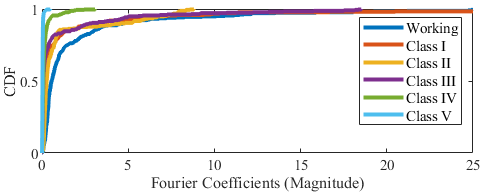
\includegraphics[width=\linewidth]{figures/2-PIR-Fault/all-5-combined/CDF_FFT.png}
		\caption{}
		\label{fig:cdf_combined_all}
	\end{subfigure}\hfill \begin{subfigure}[b]{0.16\textwidth}
		\centering
		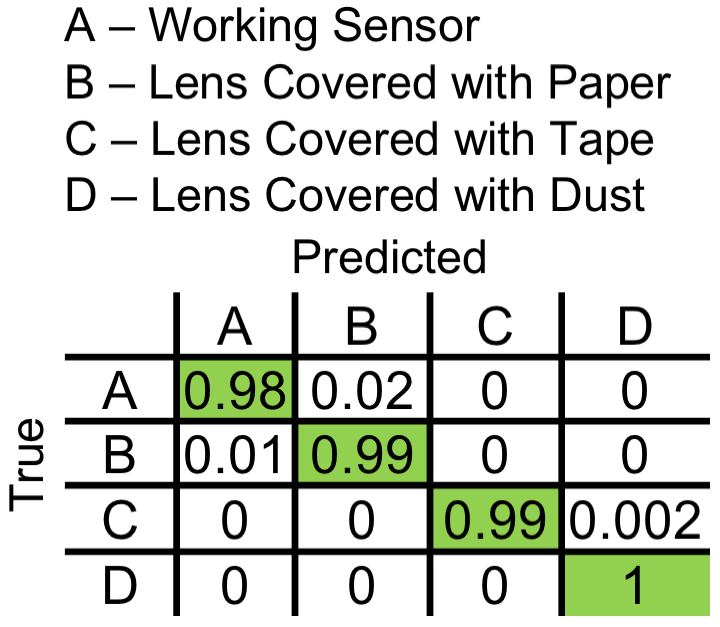
\includegraphics[width=\linewidth]{figures/classification/LensDefects/confusion-matrix-lensdefects.png}
		\caption{}
		\label{fig:finegrained_classification_results}
	\end{subfigure}\begin{subfigure}[t]{0.41\textwidth}
		\centering
		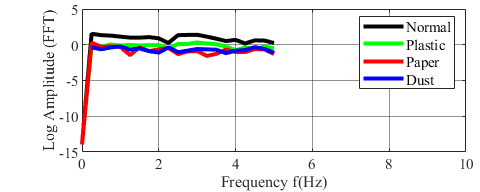
\includegraphics[width=\linewidth]{figures/classification/LensDefects/Log_Aout_Paper_Plastic_Dust_Normal.png}
		\caption{}
		\label{fig:finegrained_aout}
	\end{subfigure}
	\caption{\footnotesize{(a) CDF of FFT Coefficients showing different distributions depending on the class of faults.,(b) Fine-grained Fault Analysis,(c) \textbf{\aout} waveforms showing different behavior for paper, plastic and dust obstructions.}
	}
	\label{}
\end{figure*} \section{Discussion}

\noindent\textbf{Practicality:} We note \aout is an intrinsic signal that is present in all PIR sensors, since it is part of the sensing physics in a PIR sensor. 
However, as most applications require only binary occupancy data (\ie occupied or not occupied), some commercial-grade PIR sensors typically do not provide easy access to the \aout signal.
While \sol focuses on low-cost, commodity PIR sensors costing less than \$10-15, its physics is identical to that seen in commercial-grade PIR sensors. In fact, we obtained one such commercial PIR sensor from our building ceiling and analyzed the \aout waveform by connecting it to an oscilloscope. In our preliminary observations, we saw that the shape of \aout is similar to that in the low-cost sensors used in this paper.
Additionally, there exist some commercial sensors (\eg~\cite{panasonic_amn22111,panasonic_amn23111}) that expose \aout.
In addition, existing sensors can be modified to expose \aout --- most do as a test point on the PCB. This modification would not incur any additional hardware costs, with the exception of a new pin connector. We believe that our work can provide further incentive to other manufacturers. Lastly, our conference paper in ACM BuildSys~\cite{10.1145/3486611.3486658} was added to the product webpage by Murata electronics~\cite{murata_imx070_manual} and we hope other manufacturers use this to expose \aout in their sensor designs.

\noindent \textbf{Latency:} \sol can precisely determine if a sensor is working or faulty in single time window, which in our case comprised of 1024 samples. Since we sample at 20 Hz, the end-to-end process of data acquisition, processing and inference can be performed in a little over one minute.

\noindent\textbf{Consistency of behavior:} We observed that the inherent characteristics of the \aout signal, both in time and frequency domains, remain consistent across different manufacturers. This is expected since all PIR sensors use a pyroelectric element and the physics of operation is deterministic.

\noindent \textbf{Scale of Deployment:} Our deployment comprised of 15 sensors across various building occupancy scenarios, both in India and US, where we used a random combination of sensors in each of these deployment scenarios. While we acknowledge that our deployment scale is small-scale from the perspective of a city or a municipality spanning multiple buildings, the techniques described in this paper can be applied to a larger scale deployment comprising more sensors. To scale to larger deployments, one needs to -- \ca have edge platforms (Raspberry Pi and Arduino) located in close proximity to each of the sensor deployments (\eg in the aisle of a building for a series of rooms), \cb run wiring from each of those sensors to the edge platforms (\eg one can leverage points where PIR sensors are connected to lighting and HVAC systems) and \cc perform computation on a server on the premises of the building, such as the Building Management System (BMS), to ease the computational load on the edge platforms.

\noindent \textbf{Differentiation of Faults:} The goal of \sol is to {\em associate each faulty sensor to a failure in the corresponding sensor subsystem} shown in {\bfseries Table~\ref{tab:pir_faults}}. The classification of faults in this manner was a deliberate choice -- based on the physics of the PIR sensor, as we wanted our solution to be specific to sensors that are ubiquitous in modern buildings. Additionally, while a PIR sensor can have multiple faults present, we intentionally study faults in isolation to separate their physics and understand the impact of each of these failures on individual subsystems.

\noindent \textbf{Degradation \& Aging:} PIR sensors are susceptible to environmental elements over time, leading to degradation and aging. While we previously examined one form of degradation in \S\ref{subsec:incremental_dust}, where dust accumulation on the PIR sensor was studied, we plan to investigate additional forms of aging and degradation in the future to analyze their impact on sensor physics and the fault diagnosis process. The primary goal of this work was to understand failures and their effects on sensing physics; therefore, degradation and aging were excluded from the current analysis. However, as deployments become more long-term, these factors may play a crucial role in the analysis.

\noindent\textbf{Design:} We envision \sol to be connected to a Building Management System (BMS) and provide real-time fault detection. We envision developing APIs for application developers to build higher-level diagnostic tools on top of \sol.

\noindent \textbf{Future work and research challenges:} Gupta~\etal~\cite{Gupta2019NewMA} in the ACM LCTES'19 keynote mention the importance of fusing and navigating multiple data streams and contextualizing data streams in a CPS such as a Building Management System. They emphasize the importance of capturing taxonomy of entities (\eg data points, location and equipment) and their relationships for developing building applications. Additionally, schema systems such as BRICK~\cite{balaji2016brick}, Scrabble~\cite{10.1145/3276774.3276795} and Plaster~\cite{10.1145/3276774.3276794} are designed as solutions developed to contextualize data streams using meta-data. One could envision using \sol to enable fault diagnosis and detection in conjunction with these building-based schema systems thereby making reliability a key facet of such programming platforms. Almanee~\etal~\cite{almanee2019demo} develops a middleware, SemIoTic, that provides a semantic view of an IoT space to both the inhabitants and application developers. SemIoTic translates user-defined requests into underlying actions and can also be enhanced with the failure information from \sol. Koh~\etal~\cite{koh2019interactive} demonstrate algorithms to standardize building metadata which can become a key enabler in deploying smart building applications over heterogeneous buildings. Their key contribution is a graphical user interface with a well-defined workflow built upon a common programming interface, called Plaster. We envision that \sol can enable the integration of fault detection and diagnosis into building metadata-based schema systems. This will also improve the robustness of various downstream ML pipelines comprising the BMS that rely on the correctness and validity of data from building sensors such as the PIR sensor.




 


\section{Conclusion} 
\label{sec:concl}
The approach of using physics in conjunction with machine learning techniques can pave way for a dependable and reliable IoT. The analysis of intrinsic signals allows us to better understand the physics of a sensor that can aid in fault detection, diagnosis and maintenance of sensors. We show that in the case of PIR sensors, the appropriate use of intermediate analog signals offers potential to perform in-situ fault diagnosis thereby reducing costs and improving reliability. Due to lack of standard designs of PIR sensors, we propose that sensor vendors include the \aout signal in all PIR sensor designs to aid in the reliability of PIR sensors.
 \section*{Acknowledgments}
{We would like to thank Denizhan Kara (UIUC) and Kyo Kim (UIUC) for their insights on feature analysis. The material in this paper is based upon work supported in part by the U.S. National Science Foundation (NSF) under grant NSF CPS 2246937. Any findings, opinions, recommendations or conclusions expressed in the paper are those of the authors and do not necessarily reflect the views of sponsors.}
 \bibliographystyle{plain}
\balance
\bibliography{Sections/references.bib}
\clearpage 
\setcounter{section}{0}

\section*{\huge{\textsc{Appendix}}}
\label{sec:appendix}



\section{Frequently Asked Questions (FAQs)}
\label{sec:app}


\begin{description}[style=nextline]
	\item[Q: Where does \sol \textit{detect and diagnose} faults? ] A: \sol performs detection and diagnosis on collected data at the edge device, and does not need any additional hardware. Edge devices are commonly present in sensor deployments and are responsible to aggregate data from multiple sensors and transmit it to the cloud. We use the edge to execute \sol.
	\item[Q: Does \sol require \textit{cloud connectivity}?] 
	A: \sol performs all the computation on the edge and does not require cloud connectivity. As it detects failures on the edge and rejects incorrect data, this saves cloud-edge network bandwidth as well as ensures data from broken sensors do not reach the cloud, thereby enabling better data analytics at the cloud as well. 
	\item[Q: Does \sol detect faults at runtime? Is it instantaneous?]
	A: \sol is used to detect failures by analyzing samples over a window of 256 -- 1024 samples \ie 5 -- 20 seconds at a sampling rate of 50 Hz. Thus, it can be used to detect anomalies at runtime. In addition, \sol is non-intrusive and does not involve disassembling or uninstalling the sensor. However, the typical use case is a post-analysis \eg once in a day to find out failing sensors since edge devices are typically resource constrained.
	\item[Q: Does \sol require special sensors?]
	A: \sol requires a PIR sensor that exposes the \aout signal \ie output of pyroelectric element. Currently, not all PIR sensor manufacturers expose \aout signal in their sensor. Note however that \textit{every} PIR sensor contains the \aout signal, as it is a core part of the pyroelectric element physics. 
	\item[Q: What can PIR sensor manufacturers takeaway from \sol?]
	A: We use this work to make sensor manufacturers include the signal \aout in all their sensor designs as it would enable fault detection and diagnosis at the edge.
	\item[Q: Are the failures artificial?]
	A: It is a criticism that \sol handles only artificially-induced failures. However, this is not true. The failures induced are those observed by IoT/Smart Building technicians and engineers who deploy sensors in our buildings in US and India. We recreate these failures on cheap sensors as it is not feasible to perform large-scale deployment with expensive sensors typically seen in modern buildings.
	\item[Q: Does \sol work with high-grade PIR sensors?]
	A:  While our work focused on low-cost, commodity, large-scale, cheap deployments of PIR sensors, the physics of sensing is identical in commercial-grade PIR sensors as well. We accessed a PIR sensor from our building ceiling and analyzed the \aout waveform by connecting it to an oscilloscope. In our preliminary observations, we saw that the shape of \aout is similar to that we saw in low-cost sensors. This similarity in the nature of \aout waveforms show promise to that our analysis and techniques can be extended to commercial-grade PIR sensors as well. As each of these sensors cost around \$200, we could not study conduct a study on different failures due to their exorbitant cost.
\end{description}






















































 \end{document}
